\message{ !name(gt_problems_utf8.tex)}
\message{ !name(gt_problems_utf8.tex) !offset(-2) }
% gt_problems
% начата сортировка




% потом section заменим на mysection
\section{ Поиск выигрышной стратегии} 
% общая логика (без обратной индукции)
\problemtext{Победит тот, кто ходит первым, стратегии особой не надо\par
{\it Неизвестный участник  XXVI  Турнира имени Ломоносова}\par}


\problemtext{Здесь собраны задачи, связанные с нахождением оптимальной стратегии в играх с совершенной информацией, но без применения метода обратной индукции}

\problem{ С чего все начиналось... \par
Париж, Людовик XIV, 1654 год, высшее общество говорит о рождении новой науки - теории вероятностей. Ах, кавалер де Мере, <<fort honnete homme sans etre mathematicien>>... {\it Тигр:  <<благородный человек, хотя и не математик>>.} Старая задача, неправильные решения которой предлагались тысячелетиями (например, одно из неправильных решений предлагал изобретатель двойной записи, кумир бухгалтеров, Лука Пачоли) наконец решена правильно!\par
Два игрока играют в честную игру до шести побед. Игрок первым выигравший шесть партий (не обязательно подряд) получает 800 луидоров. К текущему моменту первый игрок выиграл 5 партий, а второй - 3 партии. Они вынуждены прервать игру в данной ситуации.\par
Как им поделить приз по справедливости? } 
\solution{100 к 700} 



\problem{ Джордж и Усама\par
Усама бен Ладен (Usama bin Laden) прячется в одной из ста пещер. Каждую ночь он меняет пещеру, в которой находится, на одну из двух соседних. Джордж Буш младший (George Bush - jr) не видит перемещений Усамы. Каждый день Буш может направить отряд спецназа в одну из пещер. \par
{\it Тигр: По-моему, это задача про ограниченную рациональность...}\par
а)	Конечны ли множества стратегий игроков?\par
б)	Может ли Буш гарантировать поимку Усамы? Если Вы считаете, что да, то укажите оптимальную стратегию; если нет, то докажите.} \solution{Джордж может поймать Усаму. Пройдемся подряд по всем пещерам, дважды осмотрим последнюю и пройдемся в обратном порядке. } 


 \problem{ Chomp! (Shuh, 1952)\par
Шоколадка разделена бороздками на дольки. Игроки ходят по очереди. За ход можно выбрать любую дольку. Выбрав дольку нужно съесть ее и все дольки расположенные выше и правее. Нижняя левая долька отравлена!\par
{\it Тигр: Зачем же продукты портить, нельзя просто крестиком пометить?}\par
а)	Верно ли, что первый игрок выигрывает на прямоугольной шоколадке любых размеров?\par
б)	Верно ли, что первый игрок выигрывает на первой четверти бесконечной шоколадки?\par
в)	Найдите оптимальную стратегию на первой четверти бесконечной шоколадки. 

Автор дополнения про бесконечную шоколадку - Роман Школлер } 
\solution{} 


\problem{ Джордж и Саддам\par
Чтобы создать завод для производства оружия массового уничтожения инженеры Саддама должны работать 3 дня на одном месте (возможно с перерывами). Каждый день Саддам выбирает место, где будет работать команда инженеров. Каждую ночь Джордж выбирает одно из мест для бомбардировки. Все потенциальные места постройки завода прекрасно просматриваются со спутника. При бомбардировке недостроенный завод полностью уничтожается. Ни один пилот не отправиться бомбить завод в ночь 13-го числа любого месяца. %воскресенье (отдых - святое!). %По соображениям политкорректности бомбардировки в ночь на день всех влюбленных не допускаются. Или субботу поставить?

Саддам выигрывает, если ему удается построить завод по производству оружия массового уничтожения. Джордж выигрывает, если не допустит этого. Может ли Саддам построить завод? Если да, то за какое время?} 
\solution{Саддам. За месяц Саддам может построить одну треть завода. За 13 месяцев у него будет 13 третей завода. Начнем их достраивать. Их тут же разрушают, но 13-ую треть мы достраиваем и 13, и 14 числа. Завод готов.}

\problem{ Жадина!\cite{zieve:tag} \par
Двое по очереди берут камни из кучки в которой находится  $N$  камней. На первом ходу разрешается взять любое число камней, но не всю кучку сразу. На последующих ходах нельзя брать больше камней, чем взял на предыдущем ходу противник. Кто выигрывает при правильной игре?\par
} \solution{} 

\problem{ <<Шестиугольники>>\par
{\it Тигр: у студентов английское название <<Нех>> почему-то вызывает нездоровую реакцию...}\par
Игровое поле поделено на правильные шестиугольники. Белые и черные ходят по очереди, занимая своей фишкой любой незанятый шестиугольник. Белые выигрывают, если им удается соединить непрерывной линией из своих фишек левую и правую сторону доски. Черные выигрывают, если им удается соединить верх и низ. Если правила остались не ясны, можно попробовать поиграть на \url{http://www.mazeworks.com/hex7/}\par
а)	Докажите, что ничья в этой игре невозможна.\par
б)	У какого игрока имеется выигрышная стратегия?\par
в)	Никто на Земле не знает, как выглядит выигрышная стратегия в <<шестиугольниках>>. Нашедшему 10 баллов по теории игр.\par
} 
\solution{а) начнем с угла вести разделительную линию, она и будет соединять две противоположные стороны б) у первого} 

\problem{ Deep Blue\par
Представим, что Вы играете партию в шахматы против компьютера. Сколько стратегий использует компьютер во время одной партии?} 
\solution{Одну. Стратегия предписывает какой ход делать в каждой конкретной ситуации. У компьютера есть программа, которая говорит железу, что делать. } 

\problem{ Modified Nim. \par
This is a modified version of the game of Nim (in the following we
assume that there is an unlimited supply of tokens.) Two players set several piles of
tokens in a row. By turns each of them takes one token from one of the piles and
adds at will as many tokens as he/she wishes to piles placed to the left of the pile
from which the token was taken. Assuming that the game ever finishes, the player
that takes the last token wins. \par
a) Prove that, no matter how they play, the game will eventually end after finitely
many steps \par
b) Find a winning strategy \par
c) Do the same for another variant of the game in which the piles are arranged in several rows (not necessarily with the same number of piles each), and players are also allowed to add any number of piles with any number of tokens each to rows placed above the one containing the pile from which the token was taken. \par
d) Generalize the problem to n-dimensional arrangements (and solve it). }
\solution{
a) Количество камней в самой правой кучке не может расти. Далее по индукции - допустим игра на $n$ кучках всегда заканчивается, а мы играем на $n+1$ кучке. Мы рано или поздно возьмем камень из самой правой ($n+1$-ой) кучки, т.к. игра на левых $n$ заканчивается. Потом еще один. И еще... \par
б) Сделать своим ходом четное число камней во всех кучках }

\problem{ Задача про выборы в совет директоров.  \par
Акционерное общество, капитал которого разделен на $N$ обыкновенных акций, проводит выборы совета директоров, в который войдут $D$ человек. Выборы проходят по кумулятивной системе: владелец $n$ акций получает при голосовании $n\cdot D$ голосов, которые он в любых пропорциях распределяет между теми кандидатами, которых он хочет видеть в совете директоров. Можно передавать кандидатам дробное количество голосов. После голосования составляется рейтинг кандидатов по убыванию количества набранных ими голосов, и в совет директоров попадают первые $D$ человек по рейтингу. При этом если на последние несколько мест претендует большее число кандидатов, набравших одинаковое количество голосов, то эти несколько мест распределяются между такими кандидатами случайным образом. \par
Сколько акций нужно иметь некоторому акционеру, чтобы гарантированно (вне зависимости от действий остальных акционеров) провести в совет директоров $d$ своих кандидатов? \par
Как изменится ответ, если акционер может передать кандидату только целое количество голосов? \par
Чему равно минимальное число акций при $N=100$, $D=15$, $d=5$? }
\solution{
Чтобы помешать акционеру провести $d$ кандидатов конкуренты должны провести $D-d+1$ своего кандидата. Оптимально распределеть имеющиеся голоса поровну.
В непрерывном случае нужно выбрать минимальное $n$ удовлетворяющее неравенству: $\frac{nD}{d}>\frac{D(N-n)}{D-d+1}$. Получаем $n_{min}= \left\lfloor \frac{Nd}{D+1}\right\rfloor+1$. \par
В непрерывном случае неравенство заменяется на
$\left\lfloor \frac{nD}{d}\right\rfloor>\left\lfloor \frac{D(N-n)}{D-d+1}\right\rfloor$ \par
Поэтому алгоритм выглядит так: 
Пробуем $n=\left\lfloor \frac{Nd}{D+1}\right\rfloor+1$ \par
Если оно подходит в неравенство, то объявляем его ответом. \par
Если оно не подходит в неравенство, то объявляем ответом $n=\left\lfloor \frac{Nd}{D+1}\right\rfloor+2$. } 
\source{Григорий Хацевич, Алексей Киселев}

\problem{ Гномы\par
Злобный дракон поймал трех гномов. И решил поиграться с ними. Каждому гному он надевает с равными вероятностями черный или белый колпак. \par
{\it Тигр: Значит дракон - это датчик случайных колпаков?} \par
Гномы видят чужие колпаки, но не видят своих и не могут общаться после выдачи колпаков. Каждый гном может попытаться угадать цвет своего колпака, либо промолчать. Дракон отпустит гномов, если хотя бы один гном угадал цвет своего колпака, и никто не сделал ошибки. Если все одновременно промолчали, или кто-нибудь ошибся, то все гномы будут съедены. Перед игрой гномы могут договориться о стратегии игры.\par
а) Как им следует играть? Какова вероятность того, что они будут спасены?\par
б) Если от далекого спутника нужно получить один бит информации (<<да>> или <<нет>>), то, отправив три бита, можно не бояться того, что природа <<испортит>> один из них. Постройте этот простой код. Проведите аналогию с предыдущим пунктом. {\it Тигр: Три гнома - три бита?}\par
Идея этой задачи используется не только при космической связи. Чтобы неглубокие царапины на компакт диске не вызывали потерь данных при записи используется код Рида-Соломона.\par
{\it Тигр: А как звали третьего гнома?}\par
} \solution{} 

\problem{ Очередь гномов\par
Злобный дракон поймал  $n$  гномов... Шляпы $k$ цветов. На этот раз гномы выстроены в ряд друг за другом. Каждый гном видит цвета шляп впереди стоящих гномов. Начиная с последнего, каждый гном называет цвет своей шляпы. Если он угадал, то он спасен.\par
Как следует играть гномам? Сколько гномов можно гарантированно спасти?
{\it Тигр: Кто последний к дракону?}} 
\solution{Последний называет остаток от деления на $k$ суммы цветов шляп впереди стоящих, гарантировано спасены $(n-1)$.} 

\problem{
Вася и Петя поступили на испытательный срок на одну работу. Они не могут координировать свои действия. У Васи 4 разные рубашки, причем два раза подряд он в одной не ходит, у Пети 5 рубашек, причем 4 точно такие же, как у Васи. Петя не хочет появиться в такой же рубашке, как и Вася. Как ему себя вести? \par
} \solution{первый день прийти в особой рубашке, затем копировать действия Васи} 

\problem{ Парадокс гладиаторов [Winkler, ТО]\par
На арене две команды гладиаторов,  $A$  и  $B$ . Каждый гладиатор обладает определенной силой, неизменной по ходу игры. В команде  $A$  всего  $N_{A} $  гладиаторов с силами  $\left\{a_{i} \right\}_{i=1}^{N_{A} } $ , в команде  $B$  -  $N_{B} $  гладиаторов с силами  $\left\{b_{i} \right\}_{i=1}^{N_{B} } $ . Игра проходит в виде последовательных турниров, в каждом из которых участвует по одному гладиатору от каждой стороны. Если в очередном турнире встречаются гладиаторы с силами  $a$  и  $b$ , то вероятность победы первого определяется величиной  $\frac{a}{a+b} $ . Гладиатор, проигравший турнир, выбывает из игры, выигравший - возвращается в команду. Исходы турниров независимы. Это означает, что гладиаторы не устают, но и не приобретают опыта. Стратегия команды предписывает, какого гладиатора выдвигать на очередной турнир в зависимости текущего состава команды. Игра ведется до полного выбывания из игры одной из команд.\par
а) Зависит ли вероятность победы команды  $A$  от используемой стратегии? Если Вы считаете, что да, то укажите оптимальную стратегию; если нет, то докажите.\par
б) Допустим, что при выборе гладиатора для очередного турнира команда может учитывать не только свой собственный текущий состав, но и состав команды-соперника. Соответственно изменяется и понятие стратегии. Будет ли зависеть вероятность победы команды от стратегии в этом случае?\par
} \solution{} 


\problem{ Парадокс гладиаторов-вампиров. [Winkler, ТO]\par
В отличие от обычного гладиатора, у победившего гладиатора-вампира сила увеличивается на силу побежденного им гладиатора-вампира. В остальном правила поединка такие же, как в предыдущей задаче.\par
Зависит ли вероятность победы команды  $A$  от используемой стратегии?\par
} \solution{} 



\problem{ Игра в шахматы [Парадоксы, О]\par
Маша и Саша играют в быстрые шахматы. У них одинаковый класс игры и оба предпочитают играть белыми, т.е. вероятность выигрыша белых  $p>0,5$ . Партии играются до 10 побед. Первую партию Маша играет белыми. Она считает, что в следующей партии белыми должен играть тот, кто выиграл предыдущую партию. Саша считает, что ходить белыми нужно по очереди. При каком варианте правил у Маши больше шансы выиграть?\par
} \solution{Игра обязательно заканчивается за 19 партий, иногда раньше. Обяжем игроков сыграть недостающие до 19 партий, даже если победитель уже определился. При этом это всегда можно сделать таким образом, чтобы Маша сыграла белыми 10 раз. Т.е. мы получаем, что при любом варианте правил, Маша играет 10 партий белыми, а Саша - 9 черными. Значит, шансы одинаковы. } 

\problem{ О пользе гадания на кофейной гуще замолвите слово... \cite{winkler:gpdp} \par
Маша пишет на бумажках два любых различных натуральных числа по своему выбору. Одну бумажку она прячет в левую руку, а другую - в правую. Саша выбирает любую Машину руку. Маша показывает число, написанное на выбранной бумажке. Саша высказывает свою догадку о том, открыл ли он большее из двух чисел или меньшее. Если Саша не угадал, то Маша выиграла.\par
а) Докажите, что у Саши не существует чистой стратегии, гарантирующей ему выигрыш более чем в 50\% случаев;\par
б) Перед выбором руки и высказыванием догадки Саша может обратиться к потомственной гадалке в пятом поколении Глафире Лукитичне\footnote{500\% гарантия, снятие порчи и сглаза без греха и ущерба для здоровья, исправляет некачественную работу шарлатанов}. Глафира Лукитична называет наугад (ничего не зная о Маше!) одно из натуральных чисел причем каждое число имеет положительную вероятность быть названным\footnote{Ну например, Глафира Лукитична в курсе геометрического или Пуассоновского распределения}. Другими словами, действия Саши (выбор левой или правой руки и высказываемая версия) могут зависеть от слов гадалки. Какую стратегию Саше следует выбрать, чтобы \underbar{гарантировать} себе (вне зависимости от действий Маши!) вероятность выигрыша строго более 50\%?\par
в)      Докажите, что услуги Глафиры Лукитичны эквивалентны использованию некоторой смешанной стратегии\par
г)      Утешьте Машу - найдите инфинум по Машиным стратегиям вероятности Сашиного выигрыша.\par
{\it Тигр: А! Вот в чем дело! А я думал, почему столько гадалок вокруг...}
} \solution{б) Выбират руку наугад. Если видимое число больше того, что сказала гадалка, говорить, что оно большее. Если гадалка попала между Машиных чисел - мы выиграли. Если нет, то у нас шансы выиграть равны 50\% г) если Маша загадывает два соседних очень больших числа, то можно приблизить вероятность машиного проигрыша к 50\% } 

\problem{ В несколько раз больше! [Binmore, О]\par
Васе предлагают две шкатулки. И обещают, что в одной из них денег в два раз больше, чем в другой. Вася открывает наугад одну из них - в ней  рублей. Вася может либо взять деньги, либо взять оставшуюся шкатулку.
а) Правильно ли Вася считает, что ожидаемое количество денег в неоткрытой шкатулке равно  $\frac{1}{2} \left(\frac{1}{2} a\right)+\frac{1}{2} \left(2a\right)=1\frac{1}{4} a$ , и, поэтому, нужно изменить свой выбор?\par
б) Пусть в пару шкатулок кладут  $3^{k} $  и  $3^{k+1} $  рублей с вероятностью  $p_{k} =\left(\frac{1}{2} \right)^{k} $. Вася выбирает наугад одну из шкатулок. Стоит ли ему изменить свой выбор, после того, как он открыл первую? Почему?\par
} \solution{а) нет, нужно считать условное ожидание, а для него нужны априорные вероятности б) для существования условного м.о. нужна конечность обычного м.о. Здесь обычное м.о. равно плюс бесконечности...} 

\section{Начнем с конца!}

\problem{ <<Забери камень>>\par
В кучке лежит 45 камней. Вася и Петя забирают камни из кучки по очереди. За один ход можно взять два, три или четыре камня. Вася ходит первым. Почетное прозвище <<Тамерлан>> получает взявший последний камень. Если в кучке остался один камень (ход по правилам сделать невозможно), то игра оканчивается ничьей.\par
{\it Тигр: А в жизни выигрывает тот, у кого куча камней больше, и совсем другим способом...}\par
а)	Классифицируйте эту игру: статическая или динамическая, с полной или неполной информацией, с совершенной или несовершенной информацией;\par
б)	Конечны ли множества стратегий игроков?\par
в)	Укажите верхнюю границу для числа стратегий игроков. Любители комбинаторики могут попытаться указать точное число стратегий.\par
г)	Кто станет Тамерланом при правильной игре?\par
д)	Кто станет Тамерланом, если это почетное прозвище получает игрок, не взявший последний камень?}
\solution{ цикл: -,+,+,+,+,-}

\problem{ <<Забери камень-2>>\par
В первой кучке - 6 камней, во второй - 7 камней. За один ход можно взять два камня или пять камней из любой кучки.\par
а)	Какой игрок выигрывает, первый или второй, если цель игры - сделать ход последним?\par
б)	Какой игрок выигрывает, если цель игры - не сделать ход последним?} 
\solution{} 


\problem{ Разные игроки\par
В кучке 121 камень. Игроки ходят по очереди. Первый игрок за один ход может взять 1 или 3 камня, а второй - 2 или 3 камня. Проигрывает тот, кто не может сделать ход по правилам. Кто выигрывает при правильной игре?}
\solution{ ++, --, ++, -+, ++, -+ и далее -+}

\problem{ Добрые пираты  \par
Полный золота торговый корабль был захвачен  $n\ge 3$  абсолютно рациональными пиратами! \par
У пиратов есть строгая иерархия: капитан, первый помощник капитана, второй помощник и т.д. Пираты делят золото так: сначала капитан предлагает свой вариант дележа, затем пираты голосуют за или против, если дележ одобрен более чем половиной пиратов (включая предложившего дележ), то он принимается, если нет, то капитана убивают, и дележ предлагает первый помощник...\par
Каждый пират хочет остаться в живых и получить побольше золота. При одинаковых выгодах для себя пират голосует за тот вариант, где в живых остается больше сотоварищей.\par
Какой дележ будет реализован (предположим, что золото бесконечно делимо)?} 
\solution{Решаем по индукции. Для удобства занумеруем пиратов начиная с самого младшего (номер 1 - зеленый юнга, ..., номер $n$ - капитан). Если в живых остался один пират, то он предлагает все себе и сам же одобряет этот дележ. Если в живых осталось два пирата ($n=2$), то предлагающий дележ должен все отдать юнге. Иначе юнга не согласится, и по правилам игры дележ не будет одобрен, а неодобренный дележ означает для пирата номер 2 смерть. Если в живых осталось три пирата, то пират номер 3 предлагает все себе. Сам он одобряет этот дележ, юнга одобряет (ему все равно ничего не достанется), только пират номер 2 против. Дележ одобрен. Если осталось $n>3$ пиратов, то пират номер $n$ предлагает все себе. Все пираты кроме пирата номер $(n-1)$ одобряют этот дележ}
\source{Мулен}

\problem{ Злые пираты \par
Торговый корабль с 100 золотых монет был захвачен $500$ абсолютно рациональными пиратами!  \par
У пиратов есть строгая иерархия: капитан, первый помощник капитана, второй помощник и т.д. Пираты делят золото так: сначала капитан предлагает свой вариант дележа, затем пираты голосуют за или против, если дележ одобрен более чем половиной пиратов, то он принимается, если нет, то капитана убивают, и дележ предлагает первый помощник...\par
Каждый пират хочет остаться в живых и получить побольше золота. При прочих равных пираты жаждут крови - чем больше других выбросят за борт, тем лучше! \par
Какой дележ будет реализован (предположим, что золотую монету не делят на меньшие части)?}
\solution{
 one of possible, the first 44 pirates are thrown overboard, and then P456 offers
 one gold piece to each of the odd-numbered pirates P1 through P199 }
\source{ \url{http://euclid.trentu.ca/math/bz/pirates_gold.pdf}}

\problem{ Скрытый Тамерлан\par
Два игрока стоят на расстоянии 1111 шагов. Они по очереди делают шаги навстречу друг другу. Вася может делать либо два, либо три шага, а Петя - либо три, либо четыре. Тот, кто первым не может сделать ход, проиграл. Начинает Вася.\par
Кто выигрывает при правильной игре?\par
} \solution{} 

\problem{ Разделяй и опустошай!\par
Есть две коробочки. В каждой из них лежит некоторое количество фишек. Игроки ходят по очереди. За один ход игрок выбрасывает содержимое одной из коробочек, и затем делит содержимое другой между двумя коробочками (как минимум одна фишка должна оставаться в каждой коробочке). Проигрывает тот, кто не может сделать ход по правилам. Найдите все выигрышные позиции.\par
} \solution{} 

\problem{ Четыреста лет назад\par
В 1612 г. в Лионе появилась книга поэта и математика Баше де Мезирьяка (Bachet? de Meziriac) <<Занимательные и приятные числовые задачи>> (Problemes plaisants et delectables qui se font par les nombres). В ней была предложена следующая игра. Двое по очереди называют числа от 1 до 10, выигрывает тот, кто первым доведет сумму до 100. Кто выигрывает при правильной игре?\par
} \solution{} 
% берем!


\problem{ Цзяньшинцзы <<Выбирание камней>>\par
Древний Китай. Две кучки камней. Игроки ходят по очереди. За один ход можно забрать либо произвольное число камней из одной кучки, либо одинаковое число камней из обеих. В одной кучке 5, а в другой - 8 камней. Кто выигрывает при правильной игре?\par
} \solution{} 

\problem{ <<Одинокий ферзь>>\par
Шахматная доска (а1 - слева внизу, h8 - вверху справа). Одинокий раненый ферзь стоит на h5. Раненый ферзь может двигаться или влево, или вниз, или влево-вниз (на любое число клеток). Двое ходят раненым ферзем по очереди. Тот, кто переставит на а1 выиграл.\par
а)	Кто выигрывает при правильной игре?\par
б)	Найдите 10 отличий игры <<Одинокий ферзь>> от игры <<Цзяньшинцзы>>\par
} \solution{} 
% берем!


\problem{ <<Набери чет>>\par
В кучке 135 камней, двое по очереди забирают себе от 1 до 4 камней. Выигрывает тот, кто к концу игры наберет четное число камней. Кто выигрывает при правильной игре?\par
} \solution{} 

\problem{ Развод [Брамс]\par
Джон и Бэтти нужно поделить виллу, яхту, акции ({\it Тигр: Контрольный пакет акций свечного заводика в Самаре}) и машина. Они условились на следующей процедуре дележа: каждый забирает себе один предмет по очереди.
Предпочтения выглядят так (в порядке убывания ценности):\par
Бэтти: яхта, вилла, акции, машина. Джон: вилла, акции, машина, яхта
а)      Найдите равновесие совершенное в подыграх, если очередность:\par
- Бэтти-Джон-Бэтти-Джон;\par
- Джон-Бэтти-Джон-Бэтти;\par
- Джон-Бэтти-Бэтти-Джон;\par
- Бэтти-Джон-Джон-Бэтти;\par
б) Изменим процедуру дележа. Джон и Бэтти одновременно называют предмет. Если их выборы различны, они получают то, что назвали; если нет, то предмет называется спорным и откладывается в особую кучу. Джон и Бэтти называют предметы до тех пор, пока остаются неподеленные предметы. Спорные предметы делят, как в предыдущем пункте, забирая по очереди. Найдите равновесия, совершенные в подыграх, для четырех вариантов очередности.\par
в) Во время дележа имущества Джон и Бэтти помирились, и решили культурно отдохнуть.\par
Предпочтения (снова в порядке убывания ценности).\par
Бэтти: театр, казино, бассейн, футбол. Джон: футбол, бассейн, казино, театр.
Они по очереди вычеркивают нежелательную альтернативу, до тех пор, пока не останется только одна. Найдите равновесия по Нэшу, совершенные в подыграх, для четырех вариантов очередности.\par
} \solution{} 

\problem{ Рулетки [Binmore, О]\par
Есть три рулетки: на первой равновероятно выпадают числа 2, 4 и 9; на второй - 1, 6 и 8; на третьей - 3, 5 и 7. Сначала первый игрок выбирает рулетку себе, затем второй игрок выбирает рулетку себе из двух оставшихся. После этого рулетки, выбранные игроками, запускаются, и случай определяет победителя. Победителем считается тот, чья рулетка покажет большее число. Победитель получает от проигравшего 100 рублей.\par
а) Нарисуйте дерево игры (можно со случайным ходом природы, можно и без - с усредненным выигрышем)\par
б) Найдите совершенное в подыграх равновесие по Нэшу\par
в) Каким игроком лучше быть в этой игре? Почему?\par
Тигр: сыр съедает вторая мышка? }
\solution{Вероятность выигрыша для второго игрока - $5/9$.}

\problem{ Рулетки [Binmore]\par
Снова три рулетки, на этот раз с числами: 2, 4, 6 и 9; 1, 5, 6 и 8; 3, 4, 5 и 7. Игроки по очереди выбирают себе рулетки. Выигрывает, тот, чья рулетка покажет большее число. Если выпадает одинаковое число, то рулетки крутятся снова.\par
Найдите совершенное в подыграх равновесие по Нэшу} 
\solution{} 

\problem{
В игре два игрока. Сначала первый игрок выбирает  $x\in {\rm R} $ , затем второй игрок, зная выбор первого, выбирает  $y\in {\rm R} $ .
Функции выигрыша имеют вид:  $u_{I} =-x^{2} +xy+9x$ ,  $u_{II} =-y^{2} -4xy+6y+5x$ .\par
а) Что представляет собой стратегия второго игрока?\par
б) Найдите равновесие по Нэшу, совершенное в подыграх;\par
в) Найдите хотя бы одно равновесие по Нэшу, не являющееся совершенным в подыграх.\par
} \solution{} 

\problem{ [Cheese-problem]\par
В выборах участвуют  $n$  человек. Каждый из них по очереди выбирает свою предвыборную позицию, число  $a_{i} \in \left[0;1\right]$ , или отказывается от участия в выборах. Ноль означает крайне левую позицию, а единица - крайне правую. После того, как каждый выбрал свою позицию, определяется победитель (возможно несколько). Каждый избиратель выбирает того кандидата, ближе к которому он находится. Доля голосующих за кандидата определяется как длина отрезка его сторонников. Если несколько кандидатов заняли одинаковую позицию, то доля голосующих делится между ними поровну. Участие в выборах приводит к небольшим издержкам.\par
а) Найдите все равновесия по Нэшу, совершенные в подыграх, для  $n=2$ .\par
б) Попробуйте  $n=3$ !\par
в) [Т] И, наконец, произвольное  $n$ .\par
{\it Тигр : первый решивший пункт <<в>> получит в приз головку сыра или 10 баллов по своему выбору .}\par
Автор: вот такие сюрпризы есть у модели линейного города.\par
} \solution{а) и б) первый и последний игроки входят на середину отрезка, остальные - не входят в) похоже так же?} 

\problem{ Кортес [О]\par
Кортес с бандой головорезов высадился на берегу. Кортес выбирает, нападать ли на деревушку или нет. Местная деревушка может либо сразу перейти в подчинение Кортеса, либо принять бой. Если деревушка примет бой, то выбор появится у Кортеса: либо драться до победного конца, либо после первых потерь бежать на кораблях обратно. Ценность деревушки для Кортеса - одна единица, ценность собственных головорезов - 2 единицы. Если Кортес будет драться до конца, то деревушка будет взята, но большинство головорезов погибнет в бою. Для жителей деревушки - главное остаться в живых, сохранить при этом независимость, конечно, желательно.\par
а) Нарисуйте дерево игры и найдите обратно-индукционный исход.\par
б) Нарисуйте дерево игры и найдите обратно-индукционный исход в случае, если Кортес ограничил свои возможности - сжег корабли.\par
в) Объясните, почему ограничение собственных возможностей приводит к таким последствиям \par
} \solution{} 

\problem{ Разборчивая невеста\par
К принцессе случайным образом выстроилась очередь из  $N$  женихов. Цель принцессы - выбрать самого богатого (даже второй по богатству жених королевства не устраивает принцессу). Женихи заходят по очереди. Когда заходит очередной претендент, принцесса узнает его годовой доход и должна либо выбрать его, либо перейти к следующему. Вернуться к предыдущему нельзя. Ничего про распределение доходов в королевстве неизвестно.
Найдите  $g_{n} $  - вероятность того, что принцесса выбрала самого богатого жениха, если известно, что она остановилась на  $n$ -ом претенденте, доход которого был больше, чем у предыдущих претендентов.
Обозначим  $h_{n} $  - вероятность выигрыша принцессы в случае, если она пропускает  $n$  первых женихов, а далее играет наилучшую стратегию. Докажите, что  $h_{n} $  не возрастает. Сравнив поведение  $g_{n} $  и  $h_{n} $ , ответьте на вопрос, какой вид имеет оптимальная стратегия. Как выглядит  $h_{n} $  левее точки  $g_{n} =h_{n} $ ? Составьте разностное уравнение на  $h_{n} $  правее точки  $g_{n} =h_{n} $ .
Найдите  $\mathop{\lim }\limits_{N\to \infty } h_{0} \left(N\right)$ .
{\it Тигр: Казалось бы, причем здесь  $e$? \par
Казалось бы, причем здесь Березовский?}} 
\solution{} 

\problem{ <<Лохотрон-2>> [Martin Shubik]\par
Несколько  $n$  игроков участвуют в аукционе. По очереди они могут повышать последнюю названную цену на натуральное число рублей или отказываться от дальнейшей игры. Игра заканчивается, когда ни один игрок не хочет повышать цену. Приз ценностью  $v$  рублей получает игрок предложивший наибольшую цену. Деньги платят {\it два} игрока: игрок назвавший наибольшую цену и игрок назвавший вторую по величине цену. У каждого игрока в распоряжении только  $b$  рублей. Для однозначности предположим, что игрок предпочитает просто потерять  $x$  рублей, нежели заплатить  $\left(x+b\right)$  рублей и выиграть  $b$  рублей.\par
а) Найдите равновесие по Нэшу, совершенное в подыграх, для  $v=10$ ,  $b=30$  и  $n=2$ ;\par
б) Найдите равновесие по Нэшу, совершенное в подыграх для произвольных  $v$ ,  $b$  и  $n$\par
} \solution{} 

\problem{ Добрая мама \par
У мамы и у дочки есть в распоряжении суммы денег  $100$  и  $10$ , соответственно. Дочка выбирает текущий объем потребления, все остальное она кладет в банк под ставку  $r=10\%$  и получает деньги в следующем периоде. В следующем периоде расходы на потребление дочки складываются из ее сбережений и трансферта  $t$  от ее мамы, размер которого определяет мама. Личная полезность дочери имеет вид  $U_{d} =\ln(d-s)+0.7\cdot \ln(s\cdot(1+r)+t)$ , где  $0.7$  - это дисконт фактор. Личная полезность мамы имеет вид:  $U_{m} =ln(100-t)+\alpha \cdot U_{d} $ , где  $\alpha >0$  - альтруистичность матери. \par
а) Найдите $t$ и $s$, если решение о величине $t$ и $s$ мама и дочка принимают одновременно. \par
б) Являются ли найденные $s$ и $t$ Парето-оптимальными? \par
в) Найдите $t$ и $s$, если сначала дочь принимает решение о значении $s$, а затем, во втором периоде, мама, зная размер $s$, выбирает $t$. \par
г) Являются ли новые $s$ и $t$ Парето-оптимальными? \par
Hint: для проверки оптимальности можно рассмотреть градиенты полезностей \par
Source: $[$3.11, Gintis$]$ \par
} \solution{} 

\problem{
Два игрока играют в теннис. Сейчас счет <<ровно>>. Т.е. партия будет продолжаться до тех пор, пока один игрок не наберет отрыв в два очка. Победитель партии получит приз равный единице. При каждой подаче игроки одновременно выбирают уровень усилий. Если первый игрок выбрал уровень усилий $a\ge 0$, а второй игрок - уровень $b\ge 0$, то первый игрок выигрывает подачу с вероятностью $\frac{a}{a+b}$. Уровень усилий вычитается из полезности игрока. Дисконтирование отсутствует. \par
а) Найдите оптимальные стратегии. \par
б) Обобщите игру на случай необходимости отрыва в $n$ очков \par
Source: Lones Smith }
\solution{}

\problem{
\begin{figure}[htbp]
    \includegraphics{game.27}
\end{figure}
Первоначально фишка расположена в узле А. Игроки по очереди могут двигать фишку на один ход в направлении, указанном стрелочкой. Тот, кто не сможет сделать очередной ход, проиграл. Кто выигрывает (первый или второй игрок) при правильной игре?}
\solution{ A, C, D, E, H = +; B, F, G, I = -} 

\problem{ Волшебная шкатулка-2 \par %bld
Количество денег в волшебной шкатулке постоянно увеличивается! Время дискретно. В момент времени  $t\in \left\{1;2;3;...;100\right\}$  там находится  $2\cdot t$  рублей. Каждый из двух игроков решает, когда ему потребовать деньги. Тот кто потребует деньги первым - получает сумму полностью, тот, кто потребует вторым - не получает ничего. Если требования поступают одновременно, то игроки делят сумму в шкатулке поровну. Если никто не потребует деньги к моменту  $t=100$ , то деньги сгорают. Найдите равновесия по Нэшу, совершенные в подыграх.\par
} 
\solution{Решаем с конца. Если мы дошли до момента $t=100$, то перед нами одновременная игра. Рисуем ее матрицу, получаем что в ней есть единственное равновесие по Нэшу - это (требовать, требовать). Рассмотрим $t=99$. Для следующего шага игра уже решена, поэтому перед нами снова матрица два на два. И снова оптимальное поведение для обоих игроков - требовать деньги. Продолжаем до первого момента времени. Получаем, что единственное SPNE - это следующая пара стратегий (требовать деньги в каждый момент времени, требовать деньги в каждый момент времени).} 
\source{Osborne, 2.111}

\problem{ Счет в банке растет. В момент времени $t$ ($t=0,1,...,T$) его
величина составляет $2t$ рублей. В каждый момент времени Муж и
Жена независимо друг от друга выбирают, потребовать ли деньги, или
нет. Если требует только один игрок, то он (она) забирает весь
вклад. Если требуют оба, то вклад делится поровну. Если не
потребовал никто, то начинается следующий период. Если никто так и
не потребовал деньги к моменту $T$, то каждый получает по $T$
рублей. Найдите SPNE. } 
\solution{}


\problem{ Тигры и волшебная антилопа \par % bld
На острове живут 99 тигров и одна вкусная волшебная антилопа. \par
Если тигр съест волшебную антилопу, то он сам превратится в волшебную антилопу. Мясо волшебной антилопы настолько вкусно, что любой тигр готов ради его вкуса на превращение в антилопу. Но ни один тигр не готов полностью расстаться с жизнью ради мяса антилопы. Тигры охотяться только в одиночку.\par
Что будет происходить на этом острове? \par
 }
\source{forum on www.wilmott.com, brainteasers}
\solution{ Один тигр и одна антилопа -> тигр съедает антилопу. Два тигра и одна антилопа -> тигры не едят антилопу, т.к. иначе за вкус придется заплатить жизнью. По индукции - при четном числе тигров, тигры воздерживаются от трапезы; при нечетном числе тигров один из тигров ест антилопу, а далее тигры воздерживаются от трапезы. } 



% bld
\problem{ Ребенок выбирает действие $x\in \mathbb{R}_{+}$. Доходы ребенка и
родителей определяются этим действием, обозначим их $c(x)$ и
$p(x)$ соответственно. Далее родители определяют величину
трансферта $t$. Полезность ребенка определяется как $c(x)+t$,
полезность родителей, как $\min\{c(x)+t,p(x)-t\}$, т.е. родители
заботятся и о доходе ребенка. \par
Верно ли, что в равновесии по Нэшу, совершенном в подыграх,
оптимальный выбор ребенка максимизирует семейное благосостояние?
} \solution{} 

\problem{ Два мушкетера сражаются на шпагах за Прекрасную Даму. Лишний раунд
означает издержки равные 1. Дисконт фактор равен $\delta$.
Полезность от Дамы равна $v>1$ для обоих претендентов. Если мушкетер
решает покинуть поле боя в момент времени $t$ при условии, что его
конкурент готов продолжить бой, то полезности равны: \par
$L=-(1+\delta+\delta^{2}+...+\delta^{t-1})$ - для покидающего \par
$W=-(1+\delta+\delta^{2}+...+\delta^{t-1})+v$ - для готового
продолжить схватку \par
Если оба решают покинуть поле боя одновременно, то каждый получает
платеж $L$ (Прекрасную Даму нельзя ни делить пополам, ни дисконтировать!) \par
а) Рассмотрим профиль стратегий, в котором первый игрок не
вступает в бой, а другой никогда не покидает поле боя. Является ли
он равновесием по Нэшу, совершенным в подыграх? Просто равновесием
по Нэшу? \par
б) Найдите симметричное равновесие по Нэшу в смешанных стратегиях
и проверьте, является ли оно совершенным в подыграх. 

Коммент: Позвольте Вас отдисконтировать? 

Коммент2: Зачем второму дама, если он никогда не покидает поле боя? } 
\solution{} 


\problem{ Русская рулетка [Т]

Два гусара, одна дама, одна пуля в шестизарядном револьвере...

Сначала первый гусар выбирает, отправиться ли ему в кабак (тогда он получит полезность ноль, а дама достанется другому) или приставить револьвер к виску и нажать на курок. Смерть означает полезность равную минус единице (при этом дама, естественно, достается другому). Если гусар остается жив, то право и обязанность выбора кабак/стреляться переходит ко второму. Барабан револьвера при этом не перекручивается, т.е. вероятность смерти увеличивается. Ценность дамы для одного гусара  $a$ , для другого -  $b$ .

а) Найдите равновесия в зависимости от  $a$  и  $b$ .

б) Каким игроком лучше быть, первым или вторым, в зависимости от   $a$  и  $b$ .

{\it Тигр: Настоящего джентльмена, конечно, интересует настоящая дама, } $a\gg 1$, $b\gg 1$ } 
\solution{$$\begin{array}{|c|ccc|}  \hline {} & {\left(ss\right)} & {\left(sk\right)} & {\left(kk\right)} \\  \hline {\left(sss\right)} & {\frac{1}{6} \left(3a-3;3b-2\right)} & {\frac{1}{6} \left(4a-2;2b-1\right)} & {\frac{1}{6} \left(5a-1;b\right)} \\ {\left(ssk\right)} & {\frac{1}{6} \left(2a-2;4b-2\right)} & {\frac{1}{6} \left(4a-2;2b-1\right)} & {\frac{1}{6} \left(5a-1;b\right)} \\ {\left(skk\right)} & {\frac{1}{6} \left(a-1;5b-1\right)} & {\frac{1}{6} \left(a-1;5b-1\right)} & {\frac{1}{6} \left(5a-1;b\right)} \\ {\left(kkk\right)} & {\frac{1}{6} \left(0;6b\right)} & {\frac{1}{6} \left(0;6b\right)} & {\frac{1}{6} \left(0;6b\right)} \\  \hline  \end{array}$$
$$\begin{array}{|c|ccc|}  \hline {} & {\left(ss\right)} & {\left(sk\right)} & {\left(kk\right)} \\  \hline {\left(ss\right)} & {\frac{1}{5} \left(3a-2;2b-2\right)} & {\frac{1}{5} \left(4a-1;b-1\right)} & {\frac{1}{5} \left(5a;0\right)} \\ {\left(sk\right)} & {\frac{1}{5} \left(2a-1;3b-2\right)} & {\frac{1}{5} \left(4a-1;b-1\right)} & {\frac{1}{5} \left(5a;0\right)} \\ {\left(kk\right)} & {\frac{1}{5} \left(a;4b-1\right)} & {\frac{1}{5} \left(a;4b-1\right)} & {\frac{1}{5} \left(5a;0\right)} \\  \hline  \end{array}$$
 $\begin{array}{|c|cc|}  \hline {} & {\left(s\right)} & {\left(k\right)} \\  \hline {\left(ss\right)} & {\frac{1}{4} \left(2a-2;2b-1\right)} & {\frac{1}{4} \left(3a-1;b\right)} \\ {\left(sk\right)} & {\frac{1}{4} \left(a-1;3b-1\right)} & {\frac{1}{4} \left(3a-1;b\right)} \\ {\left(kk\right)} & {\frac{1}{4} \left(0;4b\right)} & {\frac{1}{4} \left(0;4b\right)} \\  \hline  \end{array}$  $\begin{array}{|c|cc|}  \hline {} & {\left(s\right)} & {\left(k\right)} \\  \hline {\left(s\right)} & {\frac{1}{3} \left(2a-1;b-1\right)} & {\frac{1}{3} \left(3a;0\right)} \\ {\left(k\right)} & {\frac{1}{3} \left(a;2b-1\right)} & {\frac{1}{3} \left(3a;0\right)} \\  \hline  \end{array}$  $\begin{array}{|c|c|}  \hline {} & {\left(\emptyset \right)} \\  \hline {\left(s\right)} & {\frac{1}{2} \left(a-1;b\right)} \\ {\left(k\right)} & {\frac{1}{2} \left(0;2b\right)} \\  \hline  \end{array}$} 

\problem{ Народ и правительство [О], {\bf Il faut que j'y songe encore}
На первом шаге правительство обещает уровень инфляции  $\pi ^{d} $  в следующем году. Затем народ определяет свои ожидания инфляции  $\pi ^{e} $ . {\it Тигр: Что больше  $\pi ^{e} $  или  $e^{\pi } $ ?}\par
На третьем этапе правительство выбирает уровень инфляции  $\pi $ .
Функция полезности правительства  $U=-c\pi ^{2} -\left(y-y^{p} \right)^{2} $ , где  $y^{p} $  - потенциальный уровень выпуска. {\it Тигр: А я и не знал, что правительство такое благородное!}\par
Совокупное предложение задано функцией  $u=ay^{p} +b\left(\pi -\pi ^{e} \right)$ . Константы  $a$ ,  $b$  и  $c$  - положительные.\par
Найдите равновесие по Нэшу и платежи, получаемые игроками в следующих ситуациях:\par
а)      Население верит правительству, а правительство не обязано исполнять свои обязательства.\par
б)      Население верит правительству, а правительство исполняет свои обязательства.\par
в)      Функция полезности населения имеет вид  $U=-\left(\pi -\pi ^{e} \right)^{2} $ , а правительство исполняет свои обязательства.\par
г)      Функция полезности населения имеет вид  $U=-\left(\pi -\pi ^{e} \right)^{2} $ , а правительство не обязано исполнять свои обязательства.\par
д)      Какой должна быть величина штрафа за неисполнение обязательств, чтобы в пункте г) правительство было заинтересовано в их исполнении?\par
е)      Сравните выигрыш правительства в случаях <<в>> и <<г>>. Обратите внимание на то, что в случае <<в>> у правительства нет возможности нарушать обещание, а в случае <<г>> такая возможность появляется.
} \solution{} 

\problem{ Триэль\par
Три человека решили стреляться. Они одновременно делают выстрел, каждый сам выбирает, в кого целиться. Если после первого выстрела в живых осталось больше одного человека, то выжившие снова одновременно стреляют недруг в недруга. Триэль продолжается до тех пор, пока в живых не останется один человек или пока все не погибнут. Первый попадает с вероятностью 0,9, второй  - с вероятностью 0,5, третий - с вероятностью 0,1.\par
а) В кого кому следует стрелять, чтобы максимизировать вероятность своей победы?\par
б) Найдите вероятность победы каждого игрока.\par
в) Решите задачу, если игроки делают выстрелы не одновременно, а в последовательности первый-второй-третий-первый-второй...} 
\solution{} 


\problem{Последовательная триэль (дуэль трех игроков)

Стреляются трое: Афанасий (A), Борис (B) и Станислав (C). Вероятность попадания: A - 50\%, B - 80\%, C - 100\%. Очередность стрельбы B-A-C-B-A-C-B-A-C... Т.е. сначала B стреляет в кого хочет, потом - A, если жив, стреляет в кого хочет, потом - С, если жив, стреляет в кого хочет и т.д. Триэль продолжается до тех пор, пока в живых не останется ровно один. Предположим, что специально стрелять в воздух никто не будет. 

Как будут вести себя A, B и C, если каждый хочет выиграть?

Какие при этом будут вероятности выиграша для каждого игрока?}
\solution{Когда в живых осталось только два игрока, каждый стреляет в единственного противника. Теперь рассмотрим ситуацию, когда все трое живы:

САВ. Если ходит С, то он будет убивать В, так как для С лучше стреляться один на один с А, а не с В.

АСВ. Если ходит А... Вариант раз: А промазал (не важно в кого он целился). В этом случае С убивает В и А остается один на один с С, при этом ход у А.  Вариант два: А целился в В и попал. Тогда С убивает А. Вариант три: А целился в С и попал. Тогда А остается один на один с В. Вариант три лучше, чем вариант два. Значит, если ходит А, то он стреляет в С.

ВАС. Если ходит В... Вариант раз: В промазал (не важно в кого он целился). В этом случае А стреляет в С и С, если жив, стреляет в В. Вариант два: В целился в А и попал. Тогда С убивает В. Вариант три: В целился в С и попал. В остался один на один с С. Вариант три лучше, чем вариант два. Значит, если ходит В, то он стреляет в С.

Считаем вероятности:

САВ. $P=[1/2,0,1/2]$.

АСВ. $P=0.5[1/9,8/9,0]+0.5[1/2,0,1/2]=[11/36,16/36,9/36]$

BAC. $P=0.5[5/9,4/9,0]+0.5[11/36,16/36,9/36]=[31/72,32/72,9/72]$

Мораль для последовательности ВАСВАС...: 

Меньше всего шансов выжить у С (самого сильного).

А хотел бы стрелять в воздух (но нельзя), т.к. $31/72>11/36$

В все равно стрелять ли в С или стрелять в воздух, т.к. $32/72=16/36$}




\problem{ Быть или не быть?\par
Докажите или опровергните следующие утверждения\par
а) В игре с полной и совершенной информацией вычеркивание нестрого доминируемых стратегий может привести к потере равновесия совершенного в подыграх.}
\solution{нет}

\problem{ Ковбои \par % bld
Ковбои в количестве $n$ человек выстроились по окружности. Ковбои стреляют по очереди по часовой стрелке друг за другом (сначала стреляет ковбой номер один, затем ближайший живой и т.д.). Ковбой сам выбирает, в кого стрелять. Можно стрелять в воздух. Если ковбою безразлично в кого стрелять, то он стреляет равновероятно в одну из потенциальных жертв. Ковбои стреляют без промаха, но у каждого только один патрон. Каждый ковбой хочет остаться в живых и при прочих равных убить побольше других ковбоев.\par
а) Кто в кого будет стрелять? Чему будет равна вероятность погибнуть для каждого? \par
б) Изменится ли ответ, если стрелять в воздух нельзя? \par
в) Как изменится ответ, если вероятность попадания равна $p$? \par
г) Как изменится ответ, если патроны не ограничены? }
\solution{
1 патрон, $p$: \par
при четном $n$ - стрелять равновероятно в впередистоящих \par
при нечетном $n$ - стрелять равновероятно в позадистоящих или в воздух (если позади - никого) \par
$p_{n,k}=\frac{k-1}{n-1}$ - вероятность погибнуть для ковбоя номер $k$. (при четном $n$) \par
бесконечные патроны, $p$: \par
при четном $n$ - стрелять равновероятно в остальных \par
при нечетном $n$ - стрелять в воздух }

\problem{ 
Налоговая инспекция (или преступная группировка) выбирает размер
налога $\tau$ на объем продаж. Фирма выбирает объем продаж $y$.
Выигрыш фирмы определяется по формуле $u_{firm}=(1-\tau)y-y^{2}$,
выигрыш налоговой инспекции $u_{tax}=\tau y$. \par
а) Определите выигрыши игроков, если они принимают решения
одновременнно. \par
б) Определите выигрыши игроков, если сначала принимает решение
налоговая инспекция, а затем - фирма. \par
в) Найдите Парето-оптимальную точку. Прокомментируйте. 
} \solution{} 
\source{Коковин}

\problem{ Обратно-индукционный исход и доминирование стратегий\par
Есть дерево игры с полной совершенной информацией. К нему применили обратно индукционный метод и получили множество  $A$  обратно индукционных исходов. Затем это дерево перевели в матричную форму и оказалось, что последовательным вычеркиванием строго доминируемых стратегий можно оставить только один исход  $b$ .\par
Возможно ли, что  $b\notin A$ ? Возможно ли, что  $b\ne A$ ?\par
} \solution{} 


\problem{ Передача информации в модели Курно.\par
Две фирмы по очереди выбирают объемы производства. Вторая фирма при выборе своего объема производства не знает объема, выбранного первой фирмой. После того, как обе фирмы произвели товар, рынок определяет цены в соответствии с функцией спроса  $P\left(Q\right)=1-Q$ , где  $Q=q_{1} +q_{2} $ .\par
а) Что представляет собой стратегия второй фирмы? Найдите равновесие по Нэшу. Совпадает ли оно с равновесием по Нэшу совершенным в подыграх?\par
б) Предположим теперь, что первая фирма честно декларирует выбранный ею объем выпуска. Что представляет собой стратегия второй фирмы? Найдите равновесие по Нэшу, совершенное в подыграх. Будут ли другие равновесия по Нэшу?\par
в) Сравните платежи второй фирмы в обоих вариантах модели. Почему наличие дополнительной информации снижает платеж второй фирмы? Почему не корректно рассуждение <<Полученную информацию можно не учитывать, поэтому платеж не может упасть>>?\par
} \solution{} 

\problem{ Сжигаем деньги\par
Сначала первый игрок выбирает, а не сжечь ли ему 10 рублей... \par
{\it Тигр  автору: Вы уверены, что он рациональный?} \par
Второй игрок наблюдает действия первого, а затем игроки играют в одновременную игру:\par
$$\begin{array}{|c|cc|}  \hline {} & {a} & {b} \\  \hline {a} & {\left(-100;-100\right)} & {\left(100;0\right)} \\ {b} & {\left(0;100\right)} & {\left(0;0\right)} \\  \hline  \end{array}$$
а) Найдите все равновесия по Нэшу в одновременной игре;\par
б) Сформулируйте все стратегии игроков для игры в целом;\par
в) Найдите все равновесия по Нэшу;\par
г) Верно ли, что среди равновесий совершенных в подыграх будет равновесие, в котором первый игрок сжигает деньги?
} \solution{} 


\problem{ Обещания\par
Сначала первый игрок выбирает, будет ли он правдиво декларировать свой будущий ход или не будет обещать ничего. После правдивой декларации или ее отсутствия первый и второй игроки играют в одновременную игру:\par
$$\begin{array}{|c|cc|}  \hline {} & {a} & {b} \\  \hline {a} & {\left(1;1\right)} & {\left(-1;0\right)} \\ {b} & {\left(0;-1\right)} & {\left(0;0\right)} \\  \hline  \end{array}$$
а) Найдите все равновесия по Нэшу в одновременной игре;\par
б) Сформулируйте все стратегии игроков для игры в целом;\par
в) Найдите все равновесия по Нэшу;\par
г) Найдите все равновесия, совершенные в подыграх\par
} \solution{} 

\problem{ Две сверхдержавы\par
Две сверхдержавы играют в одновременную игру и выбирают, нажимать ли красную кнопку запуска стратегических ядерных ракет, или нет. {\it Тигр: Они доиграются...} Матрица игры имеет вид:\par
$$\begin{array}{|c|cc|}  \hline {} & {press} & {not} \\  \hline {press} & {\left(-a;-a\right)} & {\left(1;-a\right)} \\ {not} & {\left(-a;1\right)} & {\left(0;0\right)} \\  \hline  \end{array}$$
а) Найдите все равновесия по Нэшу в этой игре;\par
б) Допустим, обе сверхдержавы создали системы раннего обнаружения запуска ядерных ракет. Если одна из сверхдержав не запустила ракеты, а другая - запустила, у незапустившей появляется возможность изменить свою решение. Отменить запуск по-прежнему нельзя. Найдите равновесия по Нэшу совершенные в подыграх в измененной игре;\par
в) Найдите равновесие в случае, если систему раннего обнаружения использует только одна из стран;\par
} \solution{} 


\problem{{\rm
Построить пример игры в развернутой и/или в нормальной
форме, где $INDW \not\subseteq SPE$ или доказать, что это
невозможно. }}
\solution{}
\source{БЗИ, НГУ}


\problem{{\bf Пираты.} {\em (Мулен, 1985,p.-85).} Пусть на пиратском
корабле 50 разного старшинства пиратов делят 100 кусков
золота по следующему обычаю. Старший предлагает дележ --
кому сколько. Если хотя бы половина команды (включая его)
согласна, то так и будет, иначе его выбросят за борт, а
оставшийся старшим предложит дележ, и так далее.

Предскажите, кто сколько получит, вплоть до младшего юнги
(SPE, INDW).}
\solution{}
\source{БЗИ, НГУ}

\problem{{\bf Камешки.} {\em } Пусть Анна и Борис договорились, что
из лежащих перед ними 10 камушков Анна возьмет 1 или 2, по
желанию. Потом Борис 1 или 2, и так далее, а взявший
последний камень проиграл.

Кто выиграет при идеальной игре обоих? Сохранится ли
результат, если можно брать 1 или 2 или 3? Каков общий
метод решения всех таких задач?}
\solution{}
\source{БЗИ, НГУ}


\problem{ {\bf Вариант игры Баше.} В~игре участвуют двое, ходя
по очереди (первый, второй, первый и~т.~д.). На столе лежит
$n$ камней. В~свой ход каждый из участников может изъять
$2^k$ камней ($k=0,1,2,\ldots$; естественно, нельзя снять
со стола больше, чем там есть). Выигрывает тот, кто своим
ходом оставляет пустой стол.

\begin{enumerate}

\item Пользуясь принципом Цермело, определите выигрышные и
проигрышные позиции в игре. Для этого, например, можно
исследовать несколько первых позиций и угадать
закономерность. Обязательно обоснуйте свой ответ.

\item Опишите выигрышную стратегию игрока (в~случае, если
она у него есть). Когда выигрывает первый, а когда второй?
Может ли быть ничья?

\item Пусть $n=50$ и Вам ходить. Ваши действия?

\end{enumerate}
}
\source{БЗИ, NES}
\solution{}


\problem{ {\bf Вариант игры Ним.} Снова два участника ходят по
очереди. Теперь на столе уже две кучки камней ($m$~камней
в~первой кучке и $n$~во~второй). В~свой ход игрок может
взять сколько угодно камней из одной кучки, либо одинаковое
количество из обеих. Надо обязательно взять хотя бы один
камень. Как и раньше, выигрывает тот, кто своим ходом
оставляет пустой стол.

\begin{enumerate}

\item  Опишите процесс последовательного определения
выигрышных и проигрышных позиций в этой игре. Найдите
выигрышные стратегии для малых $m$ и~$n$.

\item Пусть $m=15$, $n=7$ и Ваш ход. Как надо сыграть?

\item Тот же вопрос, если $m=8$ и $n=13$.

\end{enumerate}
}
\source{БЗИ, NES}
\solution{}


\problem{ {\bf Русская рулетка.} Два офицера русской армии
повздорили из-за одной барышни. Порешили так: в барабан
шестизарядного револьвера случайным образом помещается одна
пуля. После чего они по очереди пытаются выстрелить в себя.
Впрочем, можно и спасовать, отказавшись тогда от притязаний
на невесту. Выигравший идет делать предложение, проигравший
остается лежать убитым, спасовавший возвращается в свой
полк, что, конечно, для него предпочтительней.

\begin{enumerate}

\item Формализуйте этот конфликт как игру с {\rm
совершенной информацией}, т.~е., без информационных
множеств. При этом считайте, что застрелившийся получает
полезность~$-1$, спасовавший~---~$0$, а выигравший~---
соответственно, $a$ или~$b$, т.~е. участники по-разному
оценивают качества будущей спутницы жизни .
Предполагается, что $a>0$ и $b>0$.

\item  Решите игру по доминированию, используя алгоритм
Цермело --- Куна. Какими будут равновесные стратегии в
зависимости от параметров~$a$ и~$b$? Удобно дать ответ в
виде диаграммы в координатах $(a,b)$, на которой указаны
соответствующие области. Граничные случаи (когда кому-то
все равно, как действовать) рассматривать не надо.

\end{enumerate}
}
\source{БЗИ, NES}
\solution{}


\problem{ {\bf Когда алгоритм Цермело работает плохо.} Найдите
все совершенные по подыграм равновесия в игре
\begin{center}
\begin{picture}(90,18)
\multiput(6,17)(25,0){3}{\vector(3,-4){13}}
\multiput(6,17)(25,0){3}{\vector(1,0){23}}
\multiput(30,17)(25,0){2}{\circle*{2}}
\put(5,17){\circle{2}} \put(4,19){{\bf 1}} \put(29,19){{\bf
2}} \put(54,19){{\bf 1}} \put(20,-2){3\,,\,2}
\put(45,-2){4\,,\,1} \put(70,-2){2\,,\,3}
\put(80,16){2\,,\,0}
\end{picture}
\end{center}
Не забыли про смеси?
}
\source{БЗИ, NES}
\solution{}



\problem{ {\bf Трагедия общины: динамическая модель (поход без
завхоза).} Имеется некий объем частных благ (например,
запас продуктов питания в походе), который может
потребляться $T$~периодов. Полезность от разового
потребления $c$~единиц продукта составляет $\sqrt{c}$.
Индивидуум ценит будущее потребление наравне с настоящим,
т.~е. дисконтирование отсутствует. Как известно, в этом
случае он стремится разделить продукт поровну между
$T$~периодами.

Предположим теперь, что участников два, а~не один, и
потребляют они из одного запаса. В~каждом периоде
потребление происходит одновременно, т.~е. игроки
независимо выбирают, сколько съесть (но не более половины
от имеющегося).

\begin{enumerate}

\item Представьте это в виде игры в развернутой форме. Как
устроено дерево?

\item Как бы вы искали совершенное по подыграм равновесие в
этой игре? Указание: изобретите что-нибудь типа функций
Беллмана, найдите равновесные стратегии потребления и
выведите рекуррентные соотношения на параметры. Является ли
равновесие оптимальным по Парето?

\item Пусть $T=3$ и вначале имеется 290 единиц продукта.
Какими будут равновесные траектории потребления?

\end{enumerate}
}
\source{БЗИ, NES}
\solution{}



\problem{ {\bf Делим пирог.} Рассмотрим две модели
``справедливой'' дележки пирога между двумя соискателями.

\begin{enumerate}

\item Один режет пирог на две части, другой выбирает себе
любую из них. Описать развернутую и нормальную форму. Каков
наиболее вероятный исход игры?

\item Один режет пирог на две части и пишет на них ``$1$''
и ``$2$''. Другой в это время, отвернувшись, говорит, какую
часть ему выдать. Описать развернутую и нормальную форму.
Как Вы думаете, может ли произойти неравный раздел?
Как-нибудь обоснуйте свой ответ.

\end{enumerate} }
\source{БЗИ}
\solution{}


\problem{ {\bf Крестики и нолики.} Рассматривается игра в
обычные ``крестики-нолики'' (${3\times 3}$). Все ли знают
ее правила? Для нас сейчас неважно, кто и когда в ней
выигрывает, нас интересуют лишь различные формы, в которых
может быть представлена игра. Для простоты можете считать,
что терминальными позициями являются только те, в которых
все 9 клеток заполнены, т.~е. игра продолжается даже если
уже ясно, кто выиграл.

\begin{enumerate}

\item\label{pos} Сколько {\it позиций} имеет игра, иными
словами, сколько существует расстановок крестиков и
ноликов, которые могут возникнуть по ходу игры (и в ее
конце)?

\item\label{razv} Сколько вершин в дереве игры
(в~развернутой форме)?  Сравните с~п.~\ref{pos}.

\item Подсчитайте, хотя бы приблизительно, сколько
стратегий имеется у каждого участника в каждом из
рассмотренных представлений игры (см. пп.~\ref{pos}
и~\ref{razv}).

\end{enumerate} }
\source{БЗИ}
\solution{}

\problem{ {\bf Захват рынка.} Две фирмы $A$ и $B$ производят
некоторый товар. В~каждый момент времени $t=1,\ldots,5$
каждая фирма может произвести единицу товара либо ничего не
производить. Затраты на производство равны~$3$, а цена
продажи определяется числом~$n$ активных фирм на рынке и
составляет~$6-2n$.

\begin{enumerate}

\item Опишите развернутую форму этой игры, стратегии
участников и функции выигрыша. Сколько стратегий у каждой
фирмы?

\item Те же вопросы, если, однажды выйдя с рынка, фирма уже
не может вернуться.

\end{enumerate} }
\source{БЗИ}
\solution{}

\problem{ {\bf Рабочий и управляющий.} В игре имеются два
участника: рабочий и управляющий. Если рабочий работает, он
теряет~$1$, а управляющий получает~$3$. Иначе рабочий
ничего не теряет а управляющий теряет~$1$. Управляющий
назначает рабочему зарплату~$w$.

\begin{enumerate}

\item Пусть рабочий и управляющий принимают свои решения
одновременно. Нарисовать развернутую и нормальную форму.
Внимание: правильно понять и формализовать игру~--- входит
в задание!


\item Тот же вопрос для случая, когда рабочему известно,
сколько ему будут платить. Как Вы думаете, чем кончится
игра и кто сколько выиграет?

\end{enumerate} }
\source{БЗИ}
\solution{}




\problem{ {\rm Веревки Одиссея: ``commitment'', мультиперсонное
представление, иррациональность.} Одиссей подплывая на
корабле к острову Сирен, хотел послушать их сладкое пение,
но знал, что всякий слушающий бросается в воду, плывет к
ним и не возвращается. Этого он не хотел. Он приказал
матросам залепить уши воском, а его самого привязать к
мачте. Так он услышал Сирен, но остался капитаном.

Составить  игру, годящуюся для объяснения этой ситуации.}
\source{БЗИ}
\solution{}


\problem{ {\bf Игра входа в отрасль.}\rm Пусть есть отрасль с
функцией обратного спроса (ценой от суммарного объема) вида
$p(Y)=9-Y$ и монополистом - старожилом в этой отрасли, с
постоянными предельными издержками $\dot{c}_1(y_1)=1$
(проверьте, что монопольная цена $p^M=5$). Пусть
потенциальный новичок входя в отрасль должен сделать
невозвратные начальные капиталовложения $K=1$ и ожидает
предельные издержки $\dot{c}_2(y_2)=2$. Пусть отрасль может
просуществовать два периода (можно обобщить на $n$) и
дисконта нет: прибыли сегодня и завтра равноценны,
альтернативное вложение капитала $K$ невозможно. Старожил
обещает новичку в случае входа добиться (повышением
выпуска) снижения цены достаточно низко ($<2$), чтобы
заставить новичка прекратить производство, предполагая, что
после этого новичок банкрот и во втором периоде можно
сохранять монополию. Если же новичок войдет, то ожидается
решение Штакельберга (т.е. SPE$_{Old,New}$): лидер-
страрожил установит выпуск раньше. Стоит ли верить этой
угрозе или он блефует и можно входить? Обобщите задачу для
различных $\dot{c}_2(y_2)\neq 2, ~K\neq 1$. }
\source{БЗИ, НГУ}
\solution{}


\problem{ {\bf Игра ``Возьми или оставь'' (``сороконожка'' - повтор)}:
%\begin{figure}[h]
%\unitlength 1mm
%\input{centip.lp}
%\caption{Игра ``Возьми или оставь''.}
%\end{figure}

Пусть первый из двух игроков (Анна) может взять 4/5 общей
прибыли (то есть \$4 из \$5 на ветви $take_{a1}$) на шаге
1, тогда игра закончится, а второму - Виктору - останется
\$1. Либо можно оставить банк на столе ($leave_{a1}$). На
шаге 2 прибыль удваивается (например, ведущим), и черед
2-го выбирать: взять ли 4/5 прибыли (то есть \$8 из \$10-и)
и закончить тем самым игру, или оставить, и т.д.
Предсказывая исход для конечной (скажем, по 3 хода каждого)
игры по принципу SPE, PBE, или THPE мы увидим, что игра
тривиально закончится на 1-м шаге $take_{a1}$ с выигрышами
(1,4). А по принципу решения $PBE(\varepsilon)$ она может
дойти до конца с большой суммой прибыли. (Здесь
$\varepsilon$-- вероятность не ниже которой ожидается от
любого хода, благодаря случайному поведению типа
иррациональности).

Покажите, что $\varepsilon >1/7$ достаточно для продолжения
игры до конца (точнее, продолжения рациональных ходов до
узла $V_3$). Какое $\varepsilon$ необходимо для этого же?

2)Пусть, ситуация изменилась: игрок Victor слышал, что Анна
в подобной игре из 10-ти ходов сделала 1 иррациональный
(невыгодный, ошибочный), и ожидает, соответственно,
вероятность иррациональности около $\alpha= 1/10$.
Аналогично,  Анна слышала, что Виктор в подобной игре из
30-ти ходов сделал 2 иррациональных хода, она ожидает
вероятность иррациональности $\beta= 2/30$ (это окажется не
то же, что 1/15!). Предположим, игроки считают рациональным
{\em брать} банк, когда вероятность ошибки партнера больше
1/7 и ожидают от партнера такого же мнения. Очевидно, при
такой ``простоватой'' рациональности, Анна на первом ходу
ВОЗЬМЕТ (если не ошибется). Но если он ошибется, возьмет ли
Виктор? Он может интерпретировать {\em оставление} Анной
как ошибку, и тогда подправить свою субъективную
вероятность ошибок А до величины (1+1)/(10+1)=2/11. Либо
считать случившееся {\em оставление} рациональным ходом, и
сделать отсюда вывод о текущих гипотезах ($\beta=?$) Анны
относительно себя (Виктора). Независимо от того, верны ли
эти гипотезы, выгодно ли теперь Виктору {\em оставлять} и
пойдет ли игра до узла $V_3$?

3)По сравнению с предыдущей ситуацией, оставим Виктора
``простым'', а первого игрока предположим способным
рассчитать предыдущую ситуацию. Станет ли он на первом шаге
ОСТАВЛЯТЬ, независимо от своих гипотез о партнере
(БЛЕФОВАТЬ)? Пойдет ли игра до 6-го хода?

4)Что если теперь оба игрока ``сложные'', и В просчитывает
возможность блефа первого (считающего второго простым),
изменит ли это результат? }
\source{БЗИ, НГУ}
\solution{}


\problem{ {\rm В задаче "террорист" из учебника,
рассмотрим, как выглядит SPE в более сложном случае: при
совпадении некоторых значений выигрышей и/или при
несовершенной информации о ходах. Случай ``С" описанной
игры возможен, если террорист --- психически особенный
человек (что с ними бывает): ему все равно, жить или нет,
но приятнее умереть или жить на Кубе. Тогда возникает много
равновесий $SPE$ (все стратегии), но ни одного $SE$,
поскольку множество IND итерационно (слабо) недоминируемых
стратегий включает неэквивалентные исходы: $IND=\{
(N_Y,NB)\hence (2,1);~ (N_Y,B)\hence (0,1)\}$.

(здесь должна быть картинка но тех не ест вербатим)
% \begin{figure}[h]

%\begin{verbatim}
%C. Case, when second          D. Case, when second player
%can understand,        player can not understand, what the
%1-st move was:       what the 1-st move was:
%   Pilot    .  2                  Pilot    .   2
%           / \ 1                          / \ 0.5
%      N-Y /   \ Cuba            2, 0 N-Y /   \ Cuba 1  0
%  2  0  /     \  1  0         0.5,1    /     \    2, 0
%   1, 1 .       . 2, 2    Terr-st      .........
% NoBomb/ \B  NB/ \Bombing           NB/ \B  NB/ \Bombing
%      /   \   /   \                  /   \   /   \
%UP=  2     0 1     0           UP=  2     0 1     0
%UT=  1     1 2     2           UT=  0.5   1 2     0
%(perfect information)       (imperfect information on moves)
%\end{verbatim}

%\caption{``Camicadze''.}
%\end{figure}

В случае ``D" выигрыши различны, но неинформированность
террориста позволяет ожидать от него любых ходов. В
результате много равновесий $SPE$ (все стратегии), но ни
одного $SE$, поскольку множество IND итерационно (слабо)
недоминируемых стратегий включает неэквивалентные исходы:
$IND=\{ (N_Y,NB)\hence (2,0.5);~ (N_Y,B)\hence (0,1)\}$.} }
\source{БЗИ, НГУ}
\solution{}


\problem{Вариация на тему игры Баше. В игре участвуют двое, ходя по очереди (первый, второй, первый,...). На столе лежит $n$ камней. В свой ход каждый из участников может взять либо столько же камней, сколько было взято его партнером на предыдущем ходу, либо на один больше. На первом ходу можно брать один или два камня. Кто не может продолжать игру по правилам (из-за недостатка камней), тот проиграл.
\begin{itemize}
\item Опишите процесс последовательного определения выигрышных и проигрышных позиций в этой игре. Найдите выигрышные стратегии для малых $n$.
\item Пусть $n=14$ и ваш ход. Как надо играть?
\item  Тот же вопрос, если $n=18$.
\item Замечание. В данной задаче авторам неизвестно короткое доказательство для  расположения выигрышных и проигрышных позиций при произвольном $n$. Восполните пробел! 
\end{itemize} }
\source{НМУ, экзамен 2004, Леша Савватеев}
\solution{Выигрышные позиции при малых $n$: 1,2,3,5,7,9,10,12,14,16,18,19...

Можно заметить, что выигрышные позиции остоят друг от друга на расстояние 1 или на расстояние 2. На двумерной доске (вроде бы?)  если аккуратно действовать то можно доказать, что начиная с 6-ой разницы есть цикл разниц вида: (1-2-2-2-2-1-2-)}



\problem{Вариация на тему игры Ним. Снова два участника ходят по очереди. Теперь на столе две кучки камней ($n$ камней в первой кучке и $m$ во второй). В свой ход игрок может взять сколько угодно камней из одной кучки, либо по одному камню из обеих. Надо обязательно взять хотя бы один камень. Выигрывает тот, кто своим ходом оставляет пустой стол.
\begin{itemize}
\item Пользуясь принципом Цермело, определите выигрышные и проигрышные позиции в игре. Для этого, например, можно исследовать несколько первых позиций и угадать закономерность. Обязательно обоснуйте свой ответ.
\item Опишите выигрышную стратегию игрока (в случае, если она у него есть). Когда выигрывает первый, а когда второй?
\item Пусть $n = 98$, $m=100$ и вам ходить. Ваши действия? 
\end{itemize}}
\source{НМУ, экзамен 2004, Леша Савватеев}
\solution{}


\problem{Дуэль. Трое захотели в жёны одну и ту же девушку. Решили драться на дуэли. Дуэль протекает так: каждый период времени каждый из дуэлянтов выбирает, стрелять ли в воздух, либо в одного из своих соперников (т.е. 3 стратегии у каждого). Первый промахивается с вероятностью $\alpha$, второй — с вероятностью $\beta$, третий — с вероятностью $\gamma$. Если после пальбы остался в живых более, чем один человек, то дуэль продолжается. Падший мёртвым получает 0, единственный живой — 1. Найдите равновесие, совершенное на подыграх. Может ли быть задача разрешена по доминированию? При каких значениях параметров? (Это очень громоздкая и сложная задача. Частичные решения будут частично оценены, конечно.)}
\source{НМУ, экзамен 2004, Леша Савватеев}
\solution{}


\problem{ Вариация на тему игры с гранатой\par
\begin{figure}[ht]
    \includegraphics{game.8}
\end{figure}

а) Укажите, сколько стратегий у каждого игрока;\par
б) Приведите пример профиля стратегий, приводящего к игре  $R-B-Y$ ,  $L-A$  и  $L-B$ .\par
в) Переведите игру в матричную форму;\par
г) Найдите равновесия по Нэшу;\par
д) Укажите, какие из найденных равновесий по Нэшу являются совершенными в подыграх.} \solution{} 

\problem{
В саду растут четыре дерева:\par
а)
\begin{figure}[ht]
    \includegraphics{game.9}
\end{figure} \par
б)
\begin{figure}[ht]
    \includegraphics{game.10}
\end{figure} \par
в)  
\begin{figure}[ht]
    \includegraphics{game.11}
\end{figure} \par
г)
\begin{figure}[ht]
    \includegraphics{game.12}
\end{figure}\par
Найдите все равновесия по Нэшу;\par
Найдите все равновесия по Нэшу, совершенные в подыграх;} 
\solution{ а) NE: RB, LA; SPNE: LA, б) RXX-BB, в) AX-R, г) LX-AA, RX-AA, LX-AB} 

\problem{ Меньше подыгр - легче считать!\par
\begin{figure}[htbp]
    \includegraphics{game.33}
\end{figure}\par
а) Укажите, сколько стратегий у каждого игрока;\par
б) Переведите игру в матричную форму;\par
в) Найдите равновесия по Нэшу;\par
г) Укажите, какие из найденных равновесий по Нэшу являются совершенными в подыграх.} 
\solution{} 







\subsection{Доллар Рубинштейна}
\problem{ Равновесия по Нэшу в модели Рубинштейна\par
Саша и Маша делят доллар по Рубинштейну. Т.е. сначала Маша предлагает свой вариант дележа, затем Саша соглашается или нет, если он не соглашается, то предлагает свой вариант и т.д. Доллар можно поделить в любой пропорции.\par
а) Приведите примеры равновесий по Нэшу, в которых:\par
- Маша предлагает поделить доллар поровну на первом шаге, а Саша соглашается\par
- Маша предлагает весь доллар Саше на первом шаге, а Саша соглашается.\par
- Игра оканчивается на втором шаге\par
б) Какие из Ваших примеров являются равновесиями, совершенными в подыграх?} 
\solution{} 

\problem{ Делим неделимый доллар! [Binmore, О]\par
Рассмотрите модель Рубинштейна с неделимым долларом (дисконт факторы игроков могут быть различными). Теперь либо весь доллар достается Саше (второму игроку), либо весь - Маше.\par
а) Постройте примеры совершенных подыгровых равновесий по Нэшу, в которых:\par
- Доллар достается Маше на первом шаге\par
- Доллар достается Саше на первом шаге\par
- Доллар достается Саше на втором шаге\par
} \solution{} 

\problem{ Делим чуть-чуть делимый доллар\par
Рассмотрите модель Рубинштейна, в которой доллар можно поделить только в пропорциях  $\left(1:0\right)$ ,  $\left(0:1\right)$ ,  $\left(0,7:0,3\right)$  и  $\left(0,4:0,6\right)$ .\par
Постройте примеры совершенных подыгровых равновесий по Нэшу, в которых:\par
- Доллар будет поделен в соотношении  $\left(0,7:0,3\right)$  на первом шаге\par
- Доллар будет поделен в соотношении  $\left(0,4:0,6\right)$  на первом шаге\par
- Доллар будет поделен в соотношении  $\left(0,7:0,3\right)$  на втором шаге\par
} \solution{} 

\problem{ [LSE, 1998]\par
Саша и Маша делят доллар Рубинштейна. Сначала вариант дележа предлагает Саша, если Маша не согласна, то предлагает она. Если и Саша не одобряет машин дележ, то оба игрока получают нулевые платежи. Маша нетерпелива, ее дисконт фактор равен  $\frac{2}{3} $ .\par
а) Найдите равновесие по Нэшу, совершенное в подыграх;\par
б) Найдите все равновесия по Нэшу;\par
в) Решите задачу в предположении, что на своем ходе Маша не может запросить себе долю больше той, что Саша запросил себе на первом ходе.} 
\solution{} 

\problem{ Рассмотрите следующий вариант модели Рубинштейна. \par %bld
У обоих игроков одинаковый дисконт-фактор. Число периодов
неограничено. Если игрок соглашается с предлагаемым дележом, то
игра окончена. Если игрок не соглашается с предлагаемым дележом,
то с вероятностью $1>p>0$ игра оканчивается и никто не получает
ничего, а с вероятностью $(1-p)$ - продолжается. \par
Найдите равновесие по Нэшу, совершенное в подыграх } 
\solution{} 

\problem{[SPE в непрерывной игре: Дележ убывающего пирога].\newline
(A.Rubinstein, 1959, see also H.Varian
``Microec.Analysis").\newline
 {\em
Уезжая из дома, мать оставила двум жадным сыновьям пирог, с
таким условием. Сначала Андрей предложит дележ $a_1\in
[0,1]$ (свою долю), если Борис согласен, то так и будет,
иначе через час Борис предложит дележ $b_2\in [0,1]$ (свою
долю). Если Андрей не согласен, он через час предложит
новый дележ $a_3\in [0,1]$, и так далее. Но с каждым часом
полезность пирога убывает (возможно, от нетерпения и от
засыхания пирога) некоторым темпом, то есть через час
остается $\alpha\in (0,1)$ для Андрея и $\beta\in (0,1)$
для Бориса. То есть, если, скажем, на третьей итерации они
согласились на дележ $(a_3, b_3); ~ a_3+ b_3=1$, то
полезность Андрея от него будет $A(a_3)=\alpha^3 a_3$,
Бориса
--- $B(b_3)=\beta^3 b_3$. Зная конечный период $T$, в течение
которого пирог остается съедобен, нужно предсказать, на
какой итерации и как (рациональные и жадные) братья
поделятся (подобная игра очень типична в ситуации, когда
две фирмы способны осуществить взаимовыгодный проект, но
надо договориться о разделе прибыли, а время переговоров
означает упущенную прибыль).

Для простоты будем считать $\alpha = \beta =1/2$, Т=4, и
нарисуем дерево (если можно так выразиться) этой
непрерывной по стратегиям игры:

Решение игры в конечном простом случае (общий случай, и
бесконечный вариант игры рассмотрите самостоятельно) легко
найти с помощью ступенчатой диграммы уровней полезностей,
алгоритмом обратной индукции.

Упражнение. Предположите, что дисконты (``кофициенты
терпения") Андрея $\alpha$ и Бориса $\beta$ разные, как и в
чью пользу (терпеливого ли) изменится решение? Обобщите
решение для произвольного числа периодов Т, и для
бесконечного $T=\infty$, например, переходом к пределу.
(Проверьте $A=(1-\beta)/(1-\alpha\beta)$,
$B=(1-\alpha)\beta/(1-\alpha\beta)$.)}}
\solution{}
\source{БЗИ, НГУ}


\problem{Модель Рубинштейна. Мама испекла пирог, и оставила его в духовке своим двум сыновьям. Потом она ушла в магазин на 3 часа, и наказала: каждые полчаса, начиная с момента закрытия за ней двери, пытаться делить пирог по принципу <<один делит, другой одобряет>>. Если не одобряет, то пирог полчаса остывает в печи, а потом снова. Начинает предлагать старший сын, затем — по очереди. За время получаса пирог сохраняет долю $\alpha$ своих замечательных вкусовых свойств с точки зрения старшего брата, и $\beta$ — с точки зрения младшего. Эти параметры общеизвестны. Если мама пришла, и обнаружила неподеленный пирог (в момент прихода мамы уже делить нельзя), то она его сходу съедает сама.
\begin{itemize}
\item Найти равновесие, совершенное на подыграх;
\item Что, если мама ушла навсегда?
\end{itemize}}
\source{НМУ, экзамен 2004, Леша Савватеев}
\solution{}





\section{За обратной индукцией. Комбинаторные игры}
\problem{ Функция Шпрага-Гранди (Sprague-Grundy function, Nim-value) 

{\it Автор: Эта большая задача предназначена для тех, кто хочет познакомиться с комбинаторной теорией игр. }\par
{\it Тигр: И для тех, кто хочет научиться быстро находить выигрышную позицию с помощью заклинания Шпрага-Гранди.}\par
Комбинаторная теория игр занимается играми двух игроков, где игроки ходят по очереди, с полной совершенной информацией без случайных ходов. Например, шахматами. В комбинаторных играх не более трех исходов: ничья, победа первого игрока, победа второго игрока. Как правило, комбинаторная игра обязательно оканчивается за конечное число ходов.\par
В комбинаторной игре с обычными правилами выигрывает игрок сделавший последний ход. В комбинаторных <<поддавках>> игрок, сделавший последний ход, проигрывает.\par
Назовем {\it схемой игры} ориентированный граф, необязательно дерево, где узлы изображают возможные позиции в игре, а ребра поясняют из какой позиции в какую можно попасть. Схема игры не совпадает с деревом игры! Схема игры в отличие от дерева не сохраняет путь, которым игроки попали в заданную позицию!
а)	Пусть у одного из игроков есть выигрышная стратегия (стратегия - это предписание, какой делать в зависимости от того, какие ходы были сделаны до этого). Докажите, что у него есть выигрышная стратегия, которая является функцией только от текущей позиции, и не учитывает того, каким путем она была достигнута. \par
Назовем  $P$ -позицией, позицию выигрышную для игрока, чей ход предшествовал этой позиции (Previous player). Назовем  $N$ -позицией, позицию выигрышную для игрока, который ходит из этой позиции (Next player).\par
б)	В кучке лежит 10 камней. За один ход можно забрать 1 или 3 камня. Изобразите схему игры. Найдите  $P$ -позиции и  $N$ -позиции.\par
в)	Докажите, что при обычных правилах в комбинаторной игре верно три утверждения. \par
Любая терминальная позиция является  $P$ -позицией. 
Любая позиция предшествующая  $P$ -позиции является  $N$ -позицией. \par
Любая позиция следующая за  $P$ -позицией является  $N$ -позицией.\par
Итак, магическое заклинание! Фунция Шпрага-Гранди!  $g\left(x\right)$!\par
В конечной игре функция Шпрага-Гранди присваивает каждому узлу целое неотрицательное число.
Всем терминальным узлам присваивается ноль.
Если у всех позиций, следующих за позицией  $x$ , функция уже посчитана, то значение функции в позиции  $x$  равно минимальному целому числу не равному последующим значениям.
Например, за  $x$  следуют четыре позиции, на которых функция Шпрага-Гранди равна 0; 1; 2 и 5 соответственно. Значит  $g\left(x\right)=3$ . Формально, если  $F\left(x\right)$  - множество узлов, следующих за узлом  $x$ , то  $g\left(x\right)=\min \left\{n\in {\rm N} \cup \left\{0\right\}:\forall y\in F\left(x\right)\Rightarrow n\ne g\left(y\right)\right\}$ .
г)	Посчитайте функцию Шпрага-Гранди для пункта <<б>>;\par
д)	Докажите, что функция Шпрага-Гранди равна нулю в  $P$ -позициях и отлична от нуля в  $N$ -позициях. В доказательстве можно воспользоваться результатами пункта <<в>>;\par
е)	Верно ли, что любой ход из  $N$ -позиции уменьшает функцию Шпрага-Гранди?\par
ж)	Верно ли, что в любой  $N$ -позиции существует такой ход, который понижает функцию Шпрага-Гранди на любое возможное натуральное число?\par
Если есть несколько комбинаторных игр, то их можно сложить! \par
Игроки ходят по очереди. Ход в игре-сумме заключается в том, что игрок выбирает любую из игр-слагаемых и делает в ней один ход. При обычных правилах проигрывает тот, кто не может сделать ход ни в одной из игр-слагаемых.\par
е)	Пример игры-суммы. Имеется три кучки - по 5, 7 и 9 камней. Из первой можно брать 1 или 2 камня, из второй - 2 или 3 камня, из третьей - 3 или 4 камня. За один ход камни можно брать только из одной кучки. Игроки ходят по очереди. Данная игра является суммой трех игр. Догадайтесь каких! Для каждой из игр слагаемых рассчитайте функцию Шпрага-Гранди.\par
Функция  $xor$  означает <<исключающее или>> в двоичной записи. Пример:  
$$91\; xor\; 21=1011011_{\left(2\right)} \; xor\; 0010101_{\left(2\right)} =1001110_{\left(2\right)} =78$$ 
ж)	Вычислите  $17\; xor\; 9$ ,  $6\; xor\; 5$  и  $7\; xor\; 19$ 
Позиция в игре-сумме определяется позицией в каждой из игр-слагаемых.\par
\underbar{Теорема Шпрага-Гранди}
В игре-сумме функция Шпрага-Гранди однозначно определяется функциями Шпрага-Гранди игр-слагаемых по правилу:  $g\left(x_{1} ,x_{2} ,...,x_{n} \right)=g_{1} \left(x_{1} \right)\; xor\; g_{2} \left(x_{2} \right)\; xor\; ...\; xor\; g_{n} \left(x_{n} \right)$ .
з)	Пользуясь теоремой и зная значения функции Шпрага-Гранди в играх-слагаемых, найдите значение функции Шпрага-Гранди в игре из пункта <<е>>; Отлично ли оно от нуля? Кто выигрывает, первый или второй игрок?\par
и)	Найдите выигрышный ход! Воспользуйтесь тем, что выигрышный ход должен переводить  $N$ -позицию в  $P$ -позицию, т.е. обнулять значение функции Шпрага-Гранди.} 
\solution{е) - нет, могут быть <<плохие>> ходы \par
ж) - да, по определению функции} 

\problem{ Доказательство теоремы Шпрага-Гранди [Т]\par
\underbar{Теорема:}\par
В игре-сумме функция Шпрага-Гранди однозначно определяется функциями Шпрага-Гранди игр-слагаемых по правилу:  $g\left(x_{1} ,x_{2} ,...,x_{n} \right)=g_{1} \left(x_{1} \right)\; xor\; g_{2} \left(x_{2} \right)\; xor\; ...\; xor\; g_{n} \left(x_{n} \right)$ .
\underbar{Доказательство:}\par
Пусть  $g\left(.\right)$  - функция в игре-сумме, определяемая согласно теореме.
а)	Докажите, что в терминальных узлах игры-суммы функция  $g\left(x\right)$  действительно равна нулю.
Пусть  $x$  - некая позиция в игре-сумме, т.е.  $x=\left(x_{1} ,x_{2} ,...,x_{n} \right)$  и  $g\left(x\right)=b$ . Рассмотрим произвольное число  $a<b$ . Нужно доказать, что за позицией  $x$  существует позиция  $x'$ , такая что  $g\left(x'\right)=y$ .
Так как  $a<b$ , то двоичная запись этих чисел различна. Пусть первое различие в двоичной записи находится на  $k$-ом месте.\par
б)	Рассмотрите число  $d=a\; xor\; b$ . Что там находится на  $k$ -ом месте? Какова длина двоичной записи этого числа? Чему равно  $d\; xor\; b$ ?
в)	По определению  $b=g_{1} \left(x_{1} \right)\; xor\; g_{2} \left(x_{2} \right)\; xor\; ...\; xor\; g_{n} \left(x_{n} \right)$ . Так как на  $k$ -ом месте в числе  $b$  содержится 1, то существует такая игра, что  $g_{i} \left(x_{i} \right)$  в двоичной записи содержит 1 на  $k$ -ом месте. Для простоты пусть  $i=1$ . Докажите, что  $d\; xor\; g_{1} \left(x_{1} \right)<g_{1} \left(x_{1} \right)$.\par
Следовательно, в этой игре существует ход, переводящий позицию  $x_{1} $  в  $x'_{1} $ , что  $g_{1} \left(x'_{1} \right)=d\; xor\; g_{1} \left(x_{1} \right)$ .
г)	Тогда  $g\left(x'_{1} ,x_{2} ,...,x_{n} \right)=g_{1} \left(x'_{1} \right)\; xor\; g_{2} \left(x_{2} \right)\; xor\; ...\; xor\; g_{n} \left(x_{n} \right)=...=...=a$ . Заполните пропуск.
Т.е. у любой позиции есть следующая с любым меньшим значением функции  $g\left(.\right)$.\par
д)	Докажите самостоятельно, что ни у одной позиции нет следующей с таким же значением функции  $g\left(.\right)$.\par
Теорема доказана!\par

{\it Тигр: Во многих последующих задачах этого раздела  шаманам придется потрясти бубном и произнести заклинания Шпрага-Гранди!}

} \solution{} 

\problem{ Ним Ласкера\par
Решите задачу, предложенную Эммануилом Ласкером, чемпионом мира по шахматам с 1894 по 1921, в книге Brettspiele der Volker (1931). {\it Тигр: Не будем смешивать шахматы и теорию игр!}\par
Есть несколько кучек камней. За ход разрешается: либо взять любое положительное количество камней из одной кучки, либо поделить любую кучку на две новые непустые кучки. Проигрывает тот, кто не может сделать ход.\par
а)	Постройте функцию Шпрага-Гранди для одной кучки из  $n$  камней;\par
б)	Определите выигрышный ход в ситуации с тремя кучками из 2, 5 и 7 камней.\par
% берем!
} \solution{б) разделить кучку 7 на 1+6 или 2+5 или 3+4} 

\problem{ Очень простая задача?\par
Есть кучка из  $n$  камней. За ход ее можно разделить на две непустые кучки. Проигрывает тот, кто не может сделать ход. \par
а)	Кто выигрывает при правильной игре в зависимости от  $n$ ?\par
б)	Является ли в этой игре функция Шпрага-Гранди периодической?\par
{\it Тигр: Осенью 2004 года эта задача была по ошибке объявлена очень трудной (якобы ее решение вообще не было известно), было обещано 10 баллов за ее решение. Никто даже не попытался...}\par
в)	Попытайтесь ответить на вопросы <<а>> и <<б>> если делить можно на две непустые неравные кучки;\par
{\it Автор: Именно решение пункта <<в>> неизвестно ни одному из нескольких миллиардов жителей планеты Земля...}\par
} \solution{} 



\problem{ Rayles\par
\phantomsection \label{Rayles}
На плоскости нарисованы точки. За один ход разрешается провести замкнутую кривую проходящую через одну или две из отмеченных точек, но не пересекающую и не касающуюся уже проведенных кривых. Проигрывает тот, кто не может сделать ход.\par
а)	Докажите, что эта игра эквивалентна игре с кучками камней по правилам: За один ход можно брать из кучки один или два камня, и, при желании, разделять ее на две кучки.\par
б)	Определите правильный ход в ситуации:\par
\begin{figure}[htbp]
    \includegraphics{game.6}
\end{figure}} 
\solution{} 

\problem{ Похоже на Ним Ласкера!\par
На плоскости нарисовано  $n$  точек. За один ход разрешается провести замкнутую кривую, проходящую через несколько отмеченных точек, но не пересекающую и не касающуюся уже проведенных кривых. Проигрывает тот, кто не может сделать ход.\par
Кто выигрывает на рисунке задачи \hyperref[Rayles]{Rayles}? Если первый игрок, то определите выигрышный ход.} 
\solution{}


\problem{ Ним\footnote{Игра <<Ним>>, вероятно, появилась в Китае, однако название считается немецким (от глагола nimm - <<брать>>). Первое европейское упоминание относится к 15 веку.} \par
Классические правила игры Ним просты. Есть несколько кучек камней. За ход можно взять любое количество камней из одной кучки. Проигрывает тот, кто не может сделать ход.\par
а)	Кто выигрывает, если имеется две кучи из 11 и 22 камней?\par
б)	Кто выигрывает, если имеется 5 куч камней из 6, 7, 8, 9 и 10 камней?\par
в)	Докажите что любая сумма конечных комбинаторных игр - это Ним с определенным количеством кучек!!! Количество кучек равно количеству слагаемых. Чему соответствует количество камней в кучках?} 
\solution{} 

\problem{ Ним на лестнице (Sprague, 1937)\par
На ступеньках лестницы лежат камни. За один ход разрешается переместить любое количество камней с одной ступеньки на ступеньку ниже. Камни, попадающие на землю (ступенька номер ноль) изымаются из игры. Игроки ходят по очереди, игрок, сделавший последний ход выигрывает.\par
а)	Докажите, что данная игра эквивалентна игре Ним (см. задачу 1.13.), где кучкам камней соответствуют ступеньки с нечетными номерами. {\it Тигр: А что, четные вообще никак не влияют?!}\par
б)	Кто выигрывает в позиции [6, 7, 5, 0, 4, 1]? (На первой ступеньке лежит 6 камней, на второй - 7 камней и т.д.)\par
в)	Кто выигрывает в позиции [1, 0, 0, 2, 4, 0, 5]?\par
} \solution{} 

\problem{ Зерна на шахматной доске\par
На клетках шахматной доски лежат зерна. В одной клетке может лежать несколько зерен. Игроки ходят по очереди, за один ход можно перенести одно зерно на одну клетку вниз, или на любое количество клеток влево. Тот, кто не может сделать ход, проигрывает.\par
В начале игры по одному зерну лежит на каждой из восьми клеток самой верхней линии.\par
Кто выигрывает в этой игре?\par
{\it Тигр: Спонсор задачи РосАгроПром!} } 
\solution{} 


\problem{Загонщик овец.\par 
Трех овец нужно загнать в хлев. За один ход можно подвинуть одну любую овцу по стрелочке один раз. Проигрывает тот, кто не может сделать ход. \par 
Кто выигрывает если изначально овцы расположены так:


}
\solution{}

\problem{Строим город.

Два игрока по очереди строят город. За один ход можно построить один дом. Дом - это один или два соседних клеточки. Между соседними домами обязательно должно быть расстояние в одну незанятую клеточку. Т.е. если один игрок построил одноклеточный дом, то 8 соседних клеток занимать нельзя. Город закончен тогда, когда больше нет места для домов. Выигрывает тот, кто закончит строительство города.

Кто выигрывает, если место для города - это прямоугольник $3\times 6$?}
\solution{}


\problem{Разделяй и влавствуй!

Два игрока по очереди строят стены. Стена - это вертикальная или горизонтальная линия толщиной в одну клеточку. Стену можно строить только на еще незастроенном пространстве. Стена должна идти от <<упора>> до <<упора>>. За один ход можно построить только одну стену. Игра оканчивается, когда все свободное место занято.

Кто выигрывает на поле размера $2\times 6$, первый или второй игрок?

Если выигрывает первый, то укажите выигрышный ход.}
\solution{}


\problem{Ним со спорным камнем

Два игрока играли-играли и вдруг обнаружили, что стоят три кучки в которых 3, 5 и 7 камней, но ровно между кучками 3 и 5 лежит один камень. К какой кучке, 3 или 5, относился этот камень не понятно. Поэтому игроки решили поступить со спорным камнем так: его можно брать, только если брать камни из кучки 3 или 5. Например, если игрок решил делать ход из кучки 5, то он может взять из нее от 1 до 5 камней и дополнительно, по желанию, взять спорный камень. Кто выигрывает при правильной игре? }
\solution{}





\section{Разработка механизмов}
\problem{ Система наказаний [Game theory at work]\par
На маленькой фирме работает 10 человек. Каждый из них может работать либо старательно, либо <<спустя рукава>>. Ни один работник не хотел бы быть уволенным. Работодатель видит качество работы каждого сотрудника и заинтересован в том, чтобы все работали старательно. Проблема заключается в том, что уволить можно не более чем одного сотрудника. Этот факт прекрасно известен работникам, они понимают, что если все будут плохо работать, то уволят только одного. Как построить систему угроз увольнений, чтобы каждый работал старательно?\par
} 
\solution{Занумеруем рабочих. Делаем нумерацию общеизвестной. Публично обещаем уволить <<тунеядца>> с наименьшим номером. Все. В результате: Номеру 1 не выгодно быть тунеядцем - его уволят не глядя на других. Номеру 2 не выгодно быть тунеядцем, т.к. номер 1 тунеядцем не будет. И т.д. } 

\problem{ О Попе и работнике его Балде \par
Поп нанял Балду, чтобы тот предсказал ему погоду. Дождь будет с
вероятностью $p$. Благодаря народным приметам Балда точно знает
$p$. Поп величину $p$ не знает. Балда выдает Попу
свою оценку $\hat{p}$ вероятности дождя завтра. \par
а) Как будет вести себя Балда, если Поп выплачивает ему
награждение по принципу: если дождь действительно был, то
выплачивается $\hat{p}$, если дождя не было, то
$1-\hat{p}$? \par
б) Поп решил заставить Балду выдавать точные оценки. В случае
дождя Поп платит $f(\hat{p})$, и $f(1-\hat{p})$ в случае
сухой погоды. Какую $f$ следует выбрать Попу? \par
Подсказка: при решении задачи Поп столкнется со странным
дифференциальным уравнением, у которого много решений, но 9-ти
классов церковно-приходской школы ему вполне должно хватить для
подбора частного решения }
\solution{
Чтобы максимум $p f(\hat{p})+(1-p)f(1-\hat{p})$ был в точке
$\hat{p}=p$ необходимым условием будет:
$pf'(p)=(1-p)f'(1-p)$. \par
Если левую часть обозначить $q(p)$, то получаем уравнение
$q(p)=q(1-p)$. Берем любую функцию, симметричную относительно
$1/2$ (останется потом только проверить, что $\hat{p}=p$ - это
максимум, а не минимум). Например, подойдет $q(x)=1$, тогда
получаем $f(x)=\ln(x)$, или $q(x)=2x(1-x)$, тогда получаем
$f(x)=-x^{2}+2x$ } 

\problem{ Заработок короля\par
В стране  $n$  жителей, каждый из которых получает заработную плату в одну монету. Когда в стране победила демократия, король потерял свою власть, даже был лишен права голоса. Единственное, что он может - так это предлагать перераспределение заработной платы. Зарплата каждого жителя должна выражаться неотрицательным количеством монет, в сумме все зарплаты должны равняться  $n$ . Когда король предлагает перераспределение зарплаты, каждый житель, кроме самого короля, может проголосовать за, против или вообще не приходить на голосование. Новое распределение одобряется, если число голосов <<за>> строго больше числа голосов <<против>>.\par
Каждый житель эгоистичен, голосует <<за>>, если в новом проекте его зарплата растет, <<против>>, если падает, и не приходит на голосование, если ему предлагается одинаковая зарплата.\par
Какую зарплату в результате получит хитрый король и сколько голосований ему потребуется?} 
\solution{} 

\problem{  3 people in a room would like
to find out what is the average of their salaries, without disclosing
their individual salaries to each other. Найдите способ это сделать. }
\solution{
Guy number one makes a guesstimate of what the average salary is. Announces it out loud.
Guy number 2 computes the difference between the guessed average and his own salary. He then whispers a number that is in the range of the computed number to guy 3. Guy 3 makes the same computation, and then adds that to the number the number that was whispered to him. 3 whispers to 1. 1 makes the same computation. Whispers to 2. 2 backs out his fake number. adds in his real number. Divides by 3. Adds to the original guess.}

\problem{ Покер в чате \par
Трое заядлых игроков в покер сидят в чате. Предложите процедуру раздачи карт, при которой каждый игрок знает свои карты и не знает карт соперника. Игроки абсолютно рациональны и обладают безграничными вычислительными возможностями, поэтому использование кодов с открытым ключом (типа RSA) недопустимо. В чате можно посылать сообщения, адресованные как всем сразу, так и конкретному лицу.\par
} \solution{} 


\problem{ Пираты делят золото\cite{brams:efcdp} \par
Есть золотой песок и три пирата, но нет весов.\par
Предпочтения пиратов субъективны (действительно равные кучи могут казаться пирату неравными). Но предпочтения стабильны: если пират считал две кучи равными,  и видит, что к первой досыпали песок, то он будет считать первую кучу большей. Каждый пират может делить кучу песка на равные кучи, сравнивать несколько куч, отсыпать из большей кучи песок так, чтобы она сравнялась с меньшей.\par

Предложите конечную процедуру справедливого дележа, при которой у пиратов не было бы зависти (каждый считал бы, что его часть не меньше, чем у других).\footnote{ Комментарий: Для двух пиратов процедура выглядит так: первый делит кучи пополам по своему мнению, второй выбирает себе б{\bf {\it о}}льшую по своему мнению, первый забирает оставшуюся. Каждый пират может гарантировать себе не меньше половины по своему мнению. \par
Примо Леви <<Воспоминания смертника>> пишет, что именно так делились пайки хлеба в концентрационном лагере <<Аушвиц>> в Польше во время Второй Мировой войны. \par
Гесиод в книге <<Теогония>> (700 лет до н.э.) описывает именно такой способ деления куска мяса между Прометеем и Зевсом (Прометей делил, Зевс выбирал). \par
{\it Тигр: А у нас верхняя палата вносит законопроект, потом нижняя голосует, какой ей больше нравится... }

Кодекс поведения пиратов обычно включал принцип <<нет жертвы - нет платы>>. Заранее оговаривались доли, которые получал каждый член команды.\par
Сначала оплачивали работу хирурга (200-250 песо), корабельного плотника (100-150 песо), компенсации за увечья (600 песо за потерю правой руки, 500 - за потерю левой руки или правой ноги, 400 - за левую ногу и 100 - за глаз или палец). Остальное делилось на равные доли, причем капитан получал 5-6 долей, помощник - 2 доли, рядовые члены команды  - по одной доли, юнга - половину доли.\par
Попытки присвоить сверх своей доли строго карались\cite{brams:dps}. }} 
\solution{} 

\problem{
Есть три брата и куча рутинной работы по дому, определенная мамой. Здесь работа - антиблаго. Придумайте процедуру дележа, при которой ни один брат не завидовал бы ни одному другому. Зависть появляется, если брат считает, что у другого работы меньше, чем у него самого. \par
Уточнения: \par
Мнения братьев субъективны (т.е. даже дележ, где каждый получает ровно по одной третьей работы, может вызывать зависть у каждого брата). Мнения братьев рациональны (часть меньше целого, транзитивность). \par
Каждый брат умеет: а) делить работу на любое количество равных (по своему мнению) частей, б) сравнивать объемы работ (по своему мнению), в) при наличии двух неравных объемов работ - от большего объема работ отделять часть так, чтобы он сравнялся с меньшим\cite{peterson:epefcd}. } 
\solution{} 

\problem{ Одновременный выстрел\par
В шеренге бок о бок стоят  $n$  солдат. В ружье у каждого из них один патрон. В произвольный момент времени один из солдат получает приказ, о том, что нужно всем одновременно выстрелить вверх. Для определенности будем считать, что время дискретно, т.е. поделено на отдельные моменты. Общаться солдаты могут очень ограниченным образом: в каждый момент времени солдат может коснуться плеча соседа слева, справа, обоих или никого. Каждый солдат может запомнить только ограниченный объем информации.\par
Верно ли, что существует некий минимальный объем запоминаемой солдатом информации, который позволяет выполнить приказ для любого  $n$ ? Если да, то придумайте соответствующий алгоритм, если нет, то докажите.} 
\solution{
Разбив время на интервалы по несколько моментов, можно передавать информацию не в виде <<коснулся-не коснулся>>, а целые слова.\par
Если вычислить солдата, стоящего в центре, то задача разбивается на две задачи меньшей размерности плюс задачка об уведомлении центрального.} 
\source{Макс Петроневич}



\section{Повторяемые игры}
\problemtext{- Доктор, доктор, мы его потеряли!!!\par
- Ну, не надо так переживать, у нас их еще целая палата.\par}

\problem{ Достижимые платежи\par
Матрица базовой игры имеет вид:  $\begin{array}{|c|cc|}  \hline {} & {t_{1} } & {t_{2} } \\  \hline {l_{1} } & {\left(4;1\right)} & {\left(4;0\right)} \\ {l_{2} } & {\left(6;5\right)} & {\left(3;1\right)} \\  \hline  \end{array}$.

а)      Изобразите графически, какие платежи достижимы в повторяемой игре;

б)      Определите, являются ли достижимыми платежи  $\left(4;2\right)$ ,  $\left(3,5;0,5\right)$ ,  $\left(5;2\right)$  и  $\left(5;3\right)$ .

в)      Какие из указанных платежей могут быть реализованы на множестве смешанных стратегий?

г) $[$Т$]$ Для каждого достижимого платежа придумайте <<умную>> стратегию, которая реализует данный платеж. {\it Тигр: Насколько умную?}} 
\solution{} 

\problem{ Средний и дисконтированный платежи

Рассмотрим повторяемую игру, в которой базовая игра задана матрицей  $\begin{array}{|c|cc|}  \hline {} & {c} & {d} \\  \hline {a} & {\left(2;1\right)} & {\left(4;-4\right)} \\ {b} & {\left(-6;5\right)} & {\left(3;1\right)} \\  \hline  \end{array}$ . Дисконт фактор  $\delta =\frac{1}{3} $ .
Запишем несколько стратегий игроков:\par
 $A$ : в любой партии делать ход  $a$;\par
 $C$ : в любой партии делать ход  $c$;\par
 $AB$ : в партиях с нечетными номерами делать ход  $a$ , в партиях с четными номерами делать ход  $b$;\par
 $DC$ : в партиях с нечетными номерами делать ход  $d$ , в партиях с четными номерами делать ход  $c$.\par
а)      Определите дисконтированный и средний платеж первого и второго игроков для следующих профилей:  $\left(A;DC\right)$ ,  $\left(AB;C\right)$  и  $\left(AB;DC\right)$.} 
\solution{} 

\problem{ Повторяемая дуополия Бертрана

Дуополия Бертрана (т.е. фирмы назначают цену) повторяется бесконечное число раз. Предельные издержки обеих фирм равны нулю. Рыночный спрос описывается функцией  $Q=\max \left\{a-bP,0\right\}$ , где  $a>0$  и  $b>0$ . Весь спрос достается фирме, назначающей наименьшую цену; если фирмы назначили одинаковую цену, то спрос делится между ними поровну.

а) Найдите все значения дисконт фактора  $\delta $, при которых монопольная цена может быть реализована с помощью стратегий переключения;

б) Как изменится ответ, если число фирм будет равно $n$ ?} 
\solution{} 

\problem{ Стратегии переключения и кнута и пряника

Матрица базовой игры имеет вид:  $\begin{array}{|c|cc|}  \hline {} & {c} & {d} \\  \hline {a} & {\left(2;1\right)} & {\left(4;0\right)} \\ {b} & {\left(1;5\right)} & {\left(3;4\right)} \\  \hline  \end{array}$ .
Заметим, что хотя в базовой игре  $a$ ,  $b$ ,  $c$  и  $d$  являются стратегиями игроков, в повторяемой игре это не стратегии, а всего лишь ходы!\par
а) Сформулируйте стратегии переключения для обоих игроков;\par
б) Сформулируйте стратегии кнута и пряника для обоих игроков;\par
в) Найдите, при каких значениях дисконт фактора стратегии переключения будут составлять совершенное подыгровое равновесие по Нэшу;\par
г) Найдите, при каких значениях дисконт фактора стратегии кнута и пряника будут составлять совершенное подыгровое равновесие по Нэшу;\par
д) Найдите, при каких значениях дисконт фактора стратегия кнута и пряника первого игрока и стратегия переключения второго игрока будут составлять совершенное подыгровое равновесие по Нэшу.} 
\solution{} 

\problem{ Стратегии переключения и кнута и пряника

Матрица базовой игры имеет вид:  $\begin{array}{|c|cc|}  \hline {} & {c} & {d} \\  \hline {a} & {\left(1;2\right)} & {\left(10;0\right)} \\ {b} & {\left(-2;4\right)} & {\left(7;3\right)} \\  \hline  \end{array}$ .
а) Сформулируйте стратегии переключения для обоих игроков;\par
б) Сформулируйте стратегии кнута и пряника для обоих игроков;\par
в) Найдите, при каких значениях дисконт фактора стратегии переключения будут составлять совершенное подыгровое равновесие по Нэшу;\par
г) Найдите, при каких значениях дисконт фактора стратегии кнута и пряника будут составлять совершенное подыгровое равновесие по Нэшу.\par
д) Найдите, при каких значениях дисконт фактора стратегия кнута и пряника второго игрока и стратегия переключения первого игрока будут составлять совершенное подыгровое равновесие по Нэшу.} 
\solution{} 

\problem{ Повторяемая игра

$$\begin{array}{|c|ccc|}  \hline {} & {A} & {B} & {C} \\  \hline {A} & {\left(3;3\right)} & {\left(3;5\right)} & {\left(0;0\right)} \\ {B} & {\left(5;3\right)} & {\left(2;2\right)} & {\left(0;0\right)} \\ {C} & {\left(0;0\right)} & {\left(0;0\right)} & {\left(1;1\right)} \\  \hline  \end{array}$$
Стратегия  $AB-C$  формулируется так:\par
Играть ход  $a$  в четных партиях и ход  $b$  - в нечетных до тех пор, пока исходом игры является  $\left(a;b\right)$  или  $\left(b;a\right)$ . Если произойдет исход, отличный от  $\left(a;b\right)$  или  $\left(b;a\right)$  всегда далее играть ход  $c$ .\par
Стратегия  $BA-C$  формулируется так:\par
Играть ход  $b$  в четных партиях и ход  $a$  - в нечетных до тех пор, пока исходом игры является  $\left(a;b\right)$  или  $\left(b;a\right)$ . Если произойдет исход, отличный от  $\left(a;b\right)$  или  $\left(b;a\right)$  всегда далее играть ход  $c$ .\par
а) При каких значениях дисконт фактора пара стратегий  $\left(AB-C;BA-C\right)$  является равновесием по Нэшу?\par
б) Совершенным подыгровым равновесием по Нэшу?} 
\solution{} 

\problem{ Коровы\par
В деревне живут пять крупных фермеров. Каждый фермер решает, сколько коров купить. {\it Тигр: Как специалист, уверяю: коровы  бесконечно делимы, непрерывны, а, если помыть лапы перед обедом, то и  всюду  дифференцируемы!} Коровы пасутся на общем Большом Пастбище. Если на пастбище пасется более ста коров, то ни одна корова не дает молока. Если пасется  $N$  коров,  $N<100$ , то каждая приносит  $M_{i} =10-0,1N$  литров молока.\par
а) Найдите равновесие по Нэшу и оптимальные по Парето точки в этой игре;\par
б) Пусть данная игра повторяется каждый год. При каких значениях дисконт фактора Парето оптимальный исход, в котором фермеры получают одинаковую выручку, может быть реализован в каждой игре?\par
в) Существует ли такой дисконт фактор и совершенное подыгровое равновесие по Нэшу, что каждый год только один из фермеров покупает коров?\par
{\it Тигр: Редактор сказал, что дисконт-фактор пишется через дефис.}\par
Автор: Пусть сам задачник составляет!} 
\solution{} 

\problem{ Как велик соблазн?\par
Следующая игра повторяется два раза (величина $p>3$ ):

$$\begin{array}{|c|cccc|}  \hline {} & {t_{1} } & {t_{2} } & {t_{3} } & {t_{4} } \\  \hline {l_{1} } & {\left(3;3\right)} & {\left(0;p\right)} & {\left(0;0\right)} & {\left(-1;0\right)} \\ {l_{2} } & {\left(p;0\right)} & {\left(1;1\right)} & {\left(0;0\right)} & {\left(-1;0\right)} \\ {l_{3} } & {\left(0;-1\right)} & {\left(0;-1\right)} & {\left(1;0\right)} & {\left(-1;-1\right)} \\ {l_{4} } & {\left(0;0\right)} & {\left(0;0\right)} & {\left(0;0\right)} & {\left(0;1\right)} \\  \hline  \end{array}$$
Первый игрок придерживается стратегии:

$$s_{1} \left(h^{t} \right)=\left\{\begin{array}{l} {l_{1} ,\quad t=1} \\ {l_{3} ,\quad t=2,\; a^{1} \in \left\{\left(l_{1} ,t_{2} \right);\left(l_{1} ,t_{3} \right);\left(l_{1} ,t_{3} \right)\right\}} \\ {l_{4} ,\quad t=2,\; a^{1} \in \left\{\left(l_{2} ,t_{1} \right);\left(l_{3} ,t_{1} \right);\left(l_{4} ,t_{1} \right)\right\}} \\ {l_{2} ,\quad otherwise} \end{array}\right. $$
Второй игрок придерживается стратегии:

В первой партии сыграть  $t_{1} $ .
Если в первой партии был сыгран исход  $\left(l_{1} ;t_{1} \right)$  или оба игрока отклонились от этого исхода, то сыграть  $t_{2} $ .
Если в первой партии от исхода  $\left(l_{1} ;t_{1} \right)$  отклонился первый игрок, то сыграть  $t_{4} $ .
Если в первой партии от исхода  $\left(l_{1} ;t_{1} \right)$  отклонился второй игрок, то сыграть  $t_{3} $ .
а) Найдите все равновесия по Нэшу в чистых стратегиях в базовой игре;\par
б) Формализуйте стратегию второго игрока (по примеру стратегии первого);\par
в) При каких  $p$  указанная пара стратегий будет совершенным подыгровым равновесием по Нэшу? Просто равновесием по Нэшу?} 
\solution{} 

\problem{ Фиктивная игра (fictitious play) [Sloth, TO]\par
Рассмотрите игру:

$$\begin{array}{|c|cc|}  \hline {} & {m_{1} } & {m_{2} } \\  \hline {l_{1} } & {\left(2;0\right)} & {\left(0;2\right)} \\ {l_{2} } & {\left(0;1\right)} & {\left(1;0\right)} \\  \hline  \end{array}$$
а) Найдите все равновесия по Нэшу в этой игре.\par
Для краткости будем обозначать стратегии игроков одним числом - вероятностью выбора первой стратегии. Т.е. профиль стратегий задается парой чисел  $a=\left(x;y\right)$ , где  $x$  - вероятность, с которой первый игрок выбирает стратегию  $l_{1} $ , а  $y$  - вероятность выбора стратегии  $t_{1} $  вторым игроком. Функции наилучшего ответа обозначим  $b_{1} \left(y\right)$  и  $b_{2} \left(x\right)$  соответственно (если первый игрок безразличен между двумя стратегиями, то  $b_{1} \left(y\right)=\frac{1}{2} $ ).
Назовем {\it начальной теорией игры} профиль  $t^{0} =\left(x^{0} ;y^{0} \right)=\left(\frac{1}{2} ;\frac{1}{2} \right)$ . <<Не знаешь, как сыграть - подбрось монетку>>.\par
б) Найдите наилучший ответ каждого игрока на данную теорию игры.\par
Обозначим этот ответ  $b\left(t^{0} \right)$ . {\it Теорией игры после первого раунда} (one-round updated theory) назовем среднее между начальной теорией и наилучшим ответом на нее. Так могут думать игроки после первого опыта игры:  $t^{1} =\frac{1}{2} t^{0} +\frac{1}{2} b\left(t^{0} \right)$ . Аналогично, {\it теория игры после } $k$ {\it -го раунда} формируется по принципу:  $t^{k} =\frac{k}{k+1} t^{k-1} +\frac{1}{k+1} b\left(t^{k-1} \right)$ . Игроки придают больший вес более длительному прошлому и делают поправку на оптимальный ответ.\par
в) Сходится ли последовательность  $\left\{t^{k} \right\}$ ? Если да, то к чему?\par
г) К чему будет сходиться  $\left\{t^{k} \right\}$  при других начальных теориях игры?\par
д) Пусть стратегия  $i$ -го игрока  $t_{i}^{\infty } =\mathop{\lim }\limits_{k\to \infty } t_{i}^{k} $  приписывает положительный вес чистой стратегии  $a_{i} $ . Докажите, что  $a_{i} $  - наилучший ответ на бесконечное количество теорий  $t_{-i}^{k} $ . Т.е. существует подпоследовательность теорий, такая, что  $a_{i} $  - наилучший ответ на любую из них.\par
е) Пользуясь предыдущим результатом, докажите, что  $a_{i} $  - наилучший ответ на  $t_{-i}^{\infty } $ . Верно ли, что из этого следует, что  $t^{\infty } $  - равновесие по Нэшу?\par
ж) Обобщите Ваше доказательство на случай произвольной игры  $\left(2\times 2\right)$ .\par
з) Рассмотрите игру (Shapley's Shimmy)  $\begin{array}{|c|ccc|}  \hline {} & {m_{1} } & {m_{2} } & {m_{3} } \\  \hline {l_{1} } & {\left(0;0\right)} & {\left(0;1\right)} & {\left(1;0\right)} \\ {l_{2} } & {\left(1;0\right)} & {\left(0;0\right)} & {\left(0;1\right)} \\ {l_{3} } & {\left(0;1\right)} & {\left(1;0\right)} & {\left(0;0\right)} \\  \hline  \end{array}$ . Нарушается ли сходимость в данном случае? Почему?} 
\solution{} 

\problem{ Какая стратегия лучше?\par
С помощью компьютера проведите симуляцию, определяющую, какая стратегия в классической дилемме заключенного лучше, <<Зуб за зуб>>, стратегия переключения, стратегия кнута и пряника, случайная стратегия и т.д.
Имеется поле размером некоторого размера (например,  $100\times 100$ ), в каждой ячейке которого живет индивид, играющий определенную стратегию.
Между индивидом и его соседями проводятся фиктивные партии, и определяется победитель, получивший наибольший дисконтированный платеж. Индивид перенимает стратегию самого удачного своего соседа. По очереди перебираются все клетки и начинается следующий раунд.\par
В начале игры стратегии предписываются случайным образом.\par
Мелкие детали, отсутствующие в условии, придумайте самостоятельно.\par
{\it Тигр: А лично мне интересно кто же, все-таки, победил в битве полов?}} 
\solution{} 

\problem{
Придумайте минимум пять стратегий в бесконечно повторяемой игре, не совпадающих со стратегией переключения.} 
\solution{} 

\problem{ [LSE, 1996]

Базовая игра повторяется два раза без дисконтирования. Может ли платеж  $\left(4;4\right)$  быть получен в первой партии в совершенном подыгровом равновесии по Нэшу? Если да, то укажите соответствующий профиль стратегий.
$$\begin{array}{|c|ccc|}  \hline {} & {a} & {b} & {c} \\  \hline {a} & {\left(3;1\right)} & {\left(0;0\right)} & {\left(5;0\right)} \\ {b} & {\left(2;1\right)} & {\left(1;2\right)} & {\left(3;1\right)} \\ {c} & {\left(1;2\right)} & {\left(0;1\right)} & {\left(4;4\right)} \\  \hline  \end{array}$$
} \solution{} 

\problem{ [LSE, 2002]

Базовая игра повторяется неограниченное число раз с дисконт фактором  $\delta $ , одинаковым для обоих игроков.

$$\begin{array}{|c|ccc|}  \hline {} & {a} & {b} & {c} \\  \hline {a} & {\left(9;9\right)} & {\left(0;0\right)} & {\left(0;0\right)} \\ {b} & {\left(12;0\right)} & {\left(6;5\right)} & {\left(0;0\right)} \\ {c} & {\left(0;5\right)} & {\left(0;0\right)} & {\left(1;2\right)} \\  \hline  \end{array}$$
Стратегия  $Q$\par
Начать игру в {\it фазе 1}:\par
Сделать ход  $a$ . Если исходом партии стал  $\left(a;a\right)$ , то вернуться к фазе 1, иначе перейти к фазе 2\par
{\it Фаза 2}: Играть ход  $b$  в каждой партии.\par

Стратегия  $P$\par
Начать игру в {\it фазе 1}:\par
Сделать ход  $a$ . Если исходом партии стал  $\left(a;a\right)$ , то вернуться к фазе 1, иначе перейти к фазе  $x$ .\par
{\it Фаза } $x$ :\par
Сделать ход  $c$ . Если исходом партии стал  $\left(c;c\right)$ , то вернуться в фазу 1, иначе перейти к фазе 2.
{\it Фаза 2}: Играть ход  $b$  в каждой партии.\par
а) При каких  $\delta $  профиль стратегий  $\left(Q;Q\right)$  - равновесие по Нэшу, совершенное в подыграх?\par
б) При каких  $\delta $  профиль стратегий  $\left(P;P\right)$  - равновесие по Нэшу, совершенное в подыграх?} 
\solution{} 

\problem{
Рассмотрим повторяемую игру с дисконт-фактором  $\delta $  и матрицей базовой игры вида
$$\begin{array}{|c|cc|}  \hline {} & {c} & {d} \\  \hline {c} & {2;6} & {-1;3} \\ {d} & {4;2} & {1;5} \\  \hline  \end{array}$$
Комментарий:  $c$  и  $d$  - это ходы, а не стратегии; стратегия в повторяемой игре - это указание игроку, какой ход делать в партии с номером  $n$  в зависимости от того, что случилось в предыдущих партиях.
Подыгра - это все партии, следующие за заданной предысторией. Дисконтированные платежи игроков в подыгре обычно рассчитывают на момент вступления игроков в игру.\par
Петя (первый игрок) использует следующую стратегию:
В 1-ой партии сделать ход  $c$ ;\par
В  $n$ -ой партии ( $n\ge 2$ )\par
       - сделать ход  $c$ , если  $n$  - нечетное число;\par
       - скопировать ход противника в  $\left(n-1\right)$ -ой партии, если  $n$  - четное число.\par
Вася (второй игрок) использует следующую стратегию:\par
В 1-ой партии сделать ход  $d$ ; Во 2-ой партии сделать ход  $c$ .\par
В  $n$ -ой партии ( $n\ge 3$ )скопировать ход противника в  $\left(n-2\right)$ -ой партии.\par
а)      Выпишите исходы первых 9-и партий. Найдите дисконтированный платеж первого игрока в игре в целом.\par
б)      Допустим, что игра была начата другими игроками, которые сыграли в первых трех партиях последовательность исходов  $\left\{\left(AA\right),\left(cd\right),\left(cc\right)\right\}$ . Петя и Вася продолжают игру начиная с 4-ой партии, используя свои стратегии. Какие исходы будут сыграны в партиях №4-9?\par
в)      Как сыграют Петя и Вася в подыгре, начинающейся после  $\left\{\left(dd\right),\left(dd\right)\right\}$ ? Выпишите исходы партий №3-9. Найдите дисконтированный платеж Васи в подыгре.\par
г)      Как сыграют Петя и Вася в подыгре с предысторией  $\left\{\left(dd\right),\left(cc\right),\left(dd\right)\right\}$ ? Найдите дисконтированный платеж Пети игрока в подыгре.\par
Комментарий: вопросы <<б>> и <<в>> спрашивают об одном и том же, просто по-разному сформулированы} 
\solution{} 

\problem{
Рассмотрим повторяемую игру с дисконт-фактором  $\delta =0,5$  и матрицей базовой игры вида
$$\begin{array}{|c|cc|}  \hline {} & {c} & {d} \\  \hline {c} & {2;2} & {-1;2} \\ {d} & {2;-1} & {0;0} \\  \hline  \end{array}$$
Петя (первый игрок) и Вася (второй игрок) используют одинаковую стратегию:
В 1-ой партии сделать ход  $c$ ;\par
В  $n$ -ой партии ( $n\ge 2$ ):\par
       - сделать ход  $c$ , если во \underbar{всех} предыдущих партиях противник делал ход  $c$ ;\par
       - сделать ход  $d$ , если хотя бы в одной предыдущей партии противник сделал ход  $d$ ;\par
Эта стратегия называется <<{\it наивной стратегией переключения}>> (<<{\it naive grim trigger}>>).\par
а) Какие исходы будут происходить в партиях? Рассчитайте платежи игроков.\par
б) Может ли Петя, используя другую стратегию, получить больший платеж?\par
в) Верно ли, что указанная пара стратегий является равновесием по Нэшу?\par
г) Как сыграют Петя и Вася в подыгре с предысторией  $\left\{\left(cc\right),\left(cd\right),\left(cc\right)\right\}$ ?\par
д) Рассчитайте платежи игроков в этой подыгре.\par
е) Может ли Вася увеличить свой выигрыш в рассматриваемой подыгре?\par
ж) Является ли указанная пара стратегий равновесием по Нэшу, совершенным в подыграх?
} \solution{} 

\problem{
Рассмотрим повторяемую игру  $G$  с дисконт-фактором  $\delta $  и матрицей базовой игры вида
$$\begin{array}{|c|cc|}  \hline {} & {c} & {d} \\  \hline {c} & {2;2} & {-1;3} \\ {d} & {3;-1} & {0;0} \\  \hline  \end{array}$$
Петя (первый игрок) использует следующую стратегию:
В 1-ой партии сделать ход  $c$ ;

В  $n$ -ой партии ( $n\ge 2$ ):

       - сделать ход  $c$ , если во \underbar{всех} предыдущих партиях был сыгран исход  $\left(cc\right)$ ;
			
       - сделать ход  $d$ , если хотя бы в одной предыдущей партии не был сыгран исход  $\left(cc\right)$ ;
			
Эта стратегия называется <<{\it стратегией переключения}>> (<<{\it grim trigger}>>).

Вася (второй игрок) также использует стратегию переключения.

Рассмотрим три подыгры:  $G_{1} $  - подыгру с предысторией  $\left\{\left(cc\right),\left(cd\right),\left(cc\right)\right\}$ ,  $G_{2} $  - подыгру с предысторией  $\left\{\left(dd\right),\left(cc\right),\left(cc\right),\left(cc\right)\right\}$  и  $G_{3} $  - подыгру с предысторией  $\left\{\left(cc\right),\left(cc\right),\left(cc\right)\right\}$ .
а) Какие исходы будут происходить в самой игре  $G$ ?\par
б) Какие исходы будут происходить в подыгре  $G_{3} $ ?\par
в) Какие исходы будут происходить в подыгре  $G_{1} $ ?\par
г) Выгодно ли Пете в одиночку использовать другую стратегию в подыгре  $G_{1} $ ? Васе?\par
д) Какие исходы будут происходить в подыгре  $G_{2} $ ?\par
е) Выгодно ли Пете в одиночку использовать другую стратегию в подыгре  $G_{2} $ ? Васе?\par
ж) [Т?] Для данной игры докажите следующее утверждение:
Если при данном  $\delta $  пара стратегий переключений равновесна по Нэшу, то она также является равновесием по Нэшу, совершенным в подыграх.
} \solution{} 

\problem{
Рассмотрим повторяемую игру  $G$  с дисконт-фактором  $\delta $  и матрицей базовой игры вида
$$\begin{array}{|c|cc|}  \hline {} & {c} & {d} \\  \hline {c} & {2;2} & {-1;3} \\ {d} & {3;-1} & {0;0} \\  \hline  \end{array}$$
Некоторые стратегии можно записывать в алгоритмической форме. Рассмотрим пример.
Стратегия первого игрока имеет вид:\par
Начать 1-ую партию в состоянии 1.\par
В состоянии 1 сделать ход  $A$ .\par
Из состояния 1 перейти в:\par
- состояние 2, если был сыгран исход  $\left(cc\right)$ ;\par
- состояние 1, если был сыгран исход  $\left(cd\right)$ ;\par
- состояние 1, если был сыгран исход  $\left(dc\right)$ ;\par
       - состояние 2, если был сыгран исход  $\left(dd\right)$ ;\par
В состоянии 2 сделать ход  $d$ .\par
Из состояния 2 перейти в:\par
- состояние 1, если был сыгран исход  $\left(cc\right)$ ;\par
- состояние 2, если был сыгран исход  $\left(cd\right)$ ;\par
- состояние 2, если был сыгран исход  $\left(dc\right)$ ;\par
       - состояние 1, если был сыгран исход  $\left(dd\right)$ ;\par
Алгоритм первого игрока можно коротко записать табличкой:


\begin{tabular} {|p{43.12pt}| p{19.60pt}| p{37.52pt}| p{19.60pt}| p{31.92pt}| } \hline
   &  \multicolumn{2}{|l|}{ Состояние 1 } &  \multicolumn{2}{|l|}{ Состояние 2 } \\ \hline
 \multicolumn{2}{|l|}{ Ход } &  \multicolumn{2}{|l|}{ c } &  d  \\ \hline
 \multicolumn{2}{|l|}{ при  $\left(AA\right)$  } &  \multicolumn{2}{|l|}{ 2 } &  1  \\ \hline
 \multicolumn{2}{|l|}{ при  $\left(Ad\right)$  } &  \multicolumn{2}{|l|}{ 1 } &  2  \\ \hline
 \multicolumn{2}{|l|}{ при  $\left(dA\right)$  } &  \multicolumn{2}{|l|}{ 1 } &  2  \\ \hline
 \multicolumn{2}{|l|}{ при  $\left(dd\right)$  } &  \multicolumn{2}{|l|}{ 2 } &  1  \\ \hline
\end{tabular}

Алгоритм второго игрока имеет вид:


\begin{tabular} {|p{43.12pt}| p{19.60pt}| p{37.52pt}| p{19.60pt}| p{31.92pt}| } \hline
   &  \multicolumn{2}{|l|}{ Состояние 1 } &  \multicolumn{2}{|l|}{ Состояние 2 } \\ \hline
 \multicolumn{2}{|l|}{ Ход } &  \multicolumn{2}{|l|}{ c } &  d  \\ \hline
 \multicolumn{2}{|l|}{ при  $\left(AA\right)$  } &  \multicolumn{2}{|l|}{ 1 } &  2  \\ \hline
 \multicolumn{2}{|l|}{ при  $\left(Ad\right)$  } &  \multicolumn{2}{|l|}{ 1 } &  2  \\ \hline
 \multicolumn{2}{|l|}{ при  $\left(dA\right)$  } &  \multicolumn{2}{|l|}{ 1 } &  2  \\ \hline
 \multicolumn{2}{|l|}{ при  $\left(dd\right)$  } &  \multicolumn{2}{|l|}{ 2 } &  1  \\ \hline
\end{tabular}

Второй игрок также как и первый, начинает 1-ую партию в состоянии 1.
а) Какие исходы будут сыграны в игре  $G$ ?\par
б) В каком состоянии оказались бы игроки, если бы в первой партии был сыгран исход  $\left(cd\right)$ ?\par
Комментарий: сами игроки, конечно, такой исход бы в 1-ой партии не сыграли.\par
в) В каком состоянии оказались бы игроки, если бы в первых двух партиях были сыграны исходы  $\left\{\left(cd\right),\left(dd\right)\right\}$ ?\par
г) Какие исходы будут сыграны в подыгре с предысторией  $\left\{\left(cd\right),\left(dc\right),\left(cc\right)\right\}$ ?
д) Какие исходы будут сыграны в подыгре с предысторией  $\left\{\left(cd\right),\left(dc\right),\left(cc\right),\left(dd\right)\right\}$ ?
} \solution{} 

\problem{
Запишите в алгоритмическом виде (с помощью таблички) следующие стратегии:
а) Стратегию <<Всегда делать ход  $c$>>.\par
б) Наивную стратегию переключения;\par
в) Стратегию переключения;
} \solution{} 

\problem{ Поиск NE, SPNE в бесконечноповторяемой игре: \par
Стратегия: \par
В первой партии с (можно менять) \par
В $n$-ой партии:\par
Если в предыстории только $(c,c)$, то сыграть $c$ \par
Если в предыстории только $(c,d)$ или $(d,c)$ то сыграть $c$ в
четной партии и
$d$ в нечетной партии \par
Иначе сыгрыть $d$ \par

Стратегия антипереключения: \par
В первой партии сыграть $d$ \par
Если в предыстории только $(d,d)$, то сыграть $d$ \par
Иначе сыграть $c$ }
\solution{}

\problem{ % bld
Рассмотрим антагонистическую игру $G$: 

$\begin{array}{|c|c|c|}
& a & b \\
a & G & 2 \\
b & -1 & 10 \\
\end{array}$ \\
Если происходит исход $(a,b)$, $(b,b)$ или $(b,a)$, то игра сразу заканчивается. \par
Если оба игрока выбирают $a$, то игра начинается заноново. Но платежи дисконтируются с коэффициентом $\delta=0.5$. Если исход $(a,a)$ выбирается еще раз, то игра опять начинается заново, и платежи дисконтируются повторно. И т.д. Если оба игрока выбирают $a$ бесконечное количество раз, то каждый получает полезность 0. \par
Найдите равновесие по Нэшу в смешанных стратегиях. \par
Hint: предположите, что у игры существует цена $v$... } 
\solution{} 



\problem{ {\bf Двукратное повторение.} Рассмотрим одновременную
игру~$G_0$ с таблицей выигрышей

\begin{center}
\begin{tabular}{|c|cc|}
\hline &$X$&$Y$\\ \hline x&5,5&1,6\\ y&6,1&0,0\\ \hline
\end{tabular}
\end{center}

Представим теперь, что эта игра повторяется дважды. Все,
что происходило в первом периоде, становится общим знанием
во втором. Выигрыши первого и второго периодов суммируются
(без дисконтирования). Обозначим эту двухпериодную
игру~$G$.

\begin{enumerate}

\item Как устроено дерево этой игры? Как задаются стратегии
участников?

\item Сколько имеется чистых совершенных по подыграм
равновесий в~$G$? Указание: нужно перебрать всевозможные
варианты равновесий в подыграх второго периода, для каждого
из них прибавить выигрыши к выигрышам первого периода и
исследовать полученную однопериодную игру (будем обозначать
ее~$\tilde G$).

\item\label{z} Обратимся к смешанному расширению игры~$G$
(в поведенческих стратегиях). Пусть равновесные исходы
подыгр второго периода зафиксированы и, таким образом, игра
сведена к некоторой однопериодной игре~$\tilde G$. Может ли
профиль чистых стратегий, неравновесный в исходной
игре~$G_0$, участвовать на первом шаге в совершенном
равновесии игры~$G$? Может ли в одной и той же игре~$\tilde
G$ быть более одного равновесия, обладающего таким
свойством?

\item Более сложный вопрос: сколько всего чистых и
смешанных совершенных равновесий в игре~$G$? Указание:
достаточно выяснить, какие из игр~$\tilde G$ имеют более
одного равновесия. В~этом может помочь пункт~\ref{z}.

\end{enumerate} }
\source{БЗИ}
\solution{}

\problem{ {\bf Суперравновесия.} Рассмотрим игру с таблицей
выигрышей \begin{center}
\begin{tabular}{|c|cc|}
\hline &$a$&$b$\\ \hline $A$&0,2&2,3\\ $B$&1,0&3,1\\ \hline
\end{tabular}
\end{center}

\begin{enumerate}

\item Пусть каждый участник применяет стратегию наказания
Nash reversion (``один раз отклонишься~--- впредь буду
всегда играть равновесие Нэша''). Какие профили {\em
коррелированных} выигрышей можно реализовать таким образом
как равновесия в бесконечно повторяющейся игре?

\item Изобразите на плоскости множество коррелированных
выигрышей, достижимых в суперравновесиях в силу Народной
теоремы.

\item Рассмотрим такую попытку реализовать
выигрыши~$(2,3)$: в начальный момент играется~$(A,b)$, а
далее игрок~1 играет~$A$, если на предыдущем ходу игрок~2
сыграл~$b$ и~$B$, если~$a$; игрок~2 действует симметричным
образом: $a$, если~$B$ и~$b$, если~$A$. Является ли эта
пара стратегий равновесием Нэша в бесконечно повторяющейся
игре (при~$\delta$, достаточно близком~к~$1$)? Если да, то
является ли равновесие совершенным по подыграм?

\end{enumerate} }
\source{БЗИ}
\solution{}


\problem{
Затянувшийся семейный спор. Рассмотрим стандартный семейный спор, когда ФФ=(3,2); ФТ=(1,1); ТФ=(0,0); ТТ=(2,3). Возможно ли, что при его многократном (но конечном) повторении совершенное на подыграх равновесие будет таким, что:
\begin{itemize}
\item в первом периоде будет сделан ход ФТ;
\item в первом периоде будет сделан ход ТФ?
\end{itemize}
Опишите пример, или докажите обратное.}
\source{НМУ, экзамен 2004, Леша Савватеев}
\solution{}






\section{Статические игры} % в том числе с ходом природы, но не с частной информацией
\problemtext{Парето-оптимальный исход - это платеж, обладающий каким-либо свойством.\par
{\it Из работы на пересдаче теории игр}\par}

\problem{ Конструктор \par
Придумайте биматричную игру размером  $\left(4\times 4\right)$ , в которой с помощью вычеркивания строго доминируемых стратегий можно оставить ровно один исход, причем существует единственная последовательность вычеркиваний.} 
\solution{} 

\problem{ Конструктор\par
Придумайте биматричную игру размером  $\left(3\times 3\right)$ , в которой с помощью вычеркивания нестрого доминируемых стратегий можно оставить ровно один исход, причем результат зависит от порядка вычеркивания.\par
} \solution{} 

\problem{ Студенты и волшебная шкатулочка \par
Вася и Петя нашли волшебную шкатулочку. Если в нее положить деньги и сказать <<Ахалай Махалай>>, то сумма, лежащая в шкатулке увеличивается в полтора раза. Один недостаток: работает только раз! Петя и Вася решили поступить так: каждый положит в шкатулку сколько хочет, потом они скажут <<Ахалай Махалай>> и поделят всю сумму поровну.\par
а)	Представьте эту игру в нормальной форме. Можно ли ее представить в матричной форме? Почему?\par
б)	Найдите равновесия по Нэшу. Является ли оно равновесием в строго доминирующих стратегиях?
} 
\solution{Два игрока. Множество стратегий первого $S_{1}=[0;+\infty)$, множество стратегий второго $S_{2}=[0;+\infty)$. Платежные функции: $u_{1}=\frac{1.5(s_{1}+s_{2})}{2}-s_{1}$,  $u_{2}=\frac{1.5(s_{1}+s_{2})}{2}-s_{2}$. В матричной форме не представляется, т.к. стратегий у каждого игрока бесконечное количество. Равновесие по Нэшу $s_{1}=0$, $s_{2}=0$. Стратегия $s_{1}=0$ строго доминирует любую стратегию первого игрока, аналогично со стратегией $s_{2}=0$.}



\problem{ Фанаты и просто любители футбола \par
На футбольный матч пришли фанаты вместе с главарем и просто любители футбола. Главарю абсолютно все равно, как смотреть футбол: стоя или сидя. Остальные фанаты получают более высокую полезность когда повторяют действия главаря. Любой просто любитель футбола хочет смотреть футбол сидя, но если человек перед ним встанет и закроет обзор, то просто любителю тоже лучше встать, чтобы лучше видеть. Фанаты с главарем заняли весь первый ряд, на остальных рядах сидят просто любители.\par
Найдите равновесия по Нэшу.} 
\solution{Эту ситуацию можно смоделировать так: $n$ игроков, у каждого две стратегии: стоять или сидеть. Равновесий по Нэшу два: главарь сидит и все сидят, главарь стоит и все стоят. } 

\problem{ Детские игры\cite{ewerhart:clg} \par % это не совсем статическая игра, но вроде лучше классифицировать так
Пусть задана {\bf {\it детская}} игра (детерминистическая игра двух игроков с полной и совершенной информацией, в которой игроки ходят по очереди, а ничья исключена; например, Ним, правила которого изложены в задаче 1.2.). Запишем эту игру в матричной форме. Выигрыш первого игрока равен единице, если он выигрывает и минус единице, если проигрывает. Будем проводить вычеркивание стратегий по раундам. Один раунд означает вычеркивание нестрого доминируемых стратегий сначала за первого, затем за второго игрока.\par
а)	Докажите, что, либо у первого, либо у второго игрока есть выигрышная стратегия, т.е. стратегия, гарантирующая выигрыш вне зависимости от действий другого игрока;\par
б)	Сколько раундов вычеркивания потребуется, чтобы матрица платежей оказалась заполнена равными числами? (либо только единицами, либо только минус единицами - в зависимости от того, у кого есть выигрышная стратегия);\par
в)	Пусть в детской игре допускается ничья. Докажите, что после двух раундов вычеркиваний матрица платежей будет заполнена равными числами (на этот раз вся матрица может быть заполнена единицами, минус единицами или нулями).\par
{\it Тигр: Дилемма заключенного - это недетская игра!}\par

г) А если в детской игре $n$ возможных исходов, то сколько раундов потребуется?} 
\solution{б) 1 в) 2 г) $\left\lfloor  \frac{n+1}{2} \right\rfloor$ }

\problem{ Студенты и экзамен $[$О$]$\par
Петя и Вася прогуляли экзамен... Они знали, что профессор очень любит путешествия, и придумали для него историю про то, как они отправились в автомобильное путешествие по России и очень хотели вернуться в день экзамена, но по дороге обратно у них сломалось колесо... Профессор согласился дать им отдельный экзамен. Он посадил их по разным аудиториям и задал один и тот же вопрос: <<Какое колесо сломалось?>>\par
а)	Представьте эту игру в нормальной форме;\par
б)	Сколько равновесий по Нэшу существует в данной игре?\par
{\it Тигр: Это по правде было?}\par
} \solution{4 равновесия} 

\problem{ Дуополия Бертрана\par
Две фирмы назначают цены на свою продукцию. Предельные издержки обеих фирм равны нулю. Рыночный спрос описывается функцией  $Q=\max \left\{a-bP,0\right\}$ , где  $a>0$  и  $b>0$ . Весь спрос достается фирме, назначившей наименьшую цену; если фирмы назначили одинаковую цену, то спрос делится между ними поровну.\par
а)	Изобразите на плоскости стратегии равновесные по Нэшу и Парето оптимальные точки;} 
\solution{} 
% берем!

\problem{ Дуополия Бертрана с компенсацией! $[$О$]$\par
Грандиозное предложение! Фирмы снова одновременно назначают цены, но каждая фирма обязуется вернуть покупателю разницу в цене товара, если конкурент продает дешевле. Покупатель прекрасно осведомлен о ценах.\par
а)	Как изменятся множества равновесных по Нэшу стратегий и Парето оптимальных точек?} 
\solution{} 

\problem{
Петя задумывает одно из чисел от 1 до 5. Вася пробует угадать. Если Вася угадал, то Петя выплачивает ему соответствующее количество золотых монет (например, за угаданное число 5 платится 5 золотых монет) \par
Найдите равновесие по Нэшу. } 
\solution{} 

\problem{ Кто где...$[$Т$]$\par
Два игрока, Иван Далекий и Василий Близкий, называют одновременно любое число из отрезка  $\left[0;1\right]$ . Выигрыш Ивана Далекого (проигрыш Василия Близкого) - это расстояние между числами.\par
а)	Существуют ли равновесия по Нэшу в чистых стратегиях?\par
б)	Найдите все равновесия по Нэшу в смешанных стратегиях.} 
\solution{} 

\problem{ Делим пирог\par
Мама спрашивает двух братьев, какую часть пирога каждый хотел бы получить. Братья получают то, что попросили, если пирога хватает. Если братья вместе запросили больше, чем целый пирог, то они не получают ничего.\par
а)	Представьте игру в нормальной форме;\par
б)	Найдите все равновесия по Нэшу в чистых стратегиях.} 
\solution{} 

\problem{ Около среднего [Cramton]\par
Три игрока одновременно называют любое число из отрезка  $\left[0;1\right]$ . Выигрыш в сто рублей получает тот, чье число окажется ближе всего к среднему. Если несколько игроков оказались одинаково близки к среднему, то они делят выигрыш поровну.\par
а)	Представьте игру в нормальной форме;\par
б)	Найдите все равновесия по Нэшу в чистых стратегиях;\par
в)	Найдите все равновесия в смешанных стратегиях, если игроки могут называть только концы отрезка (числа 0 и 1);\par
г)	Найдите все равновесия по Нэшу в чистых стратегиях, если выигрывает тот, кто назовет число, наиболее удаленное от среднего.} 
\solution{} 

\problem{ Камень-Ножницы-Бумага\par
а)	Представьте игру <<Камень-Ножницы-Бумага>> в нормальной форме; {\it Тигр: Те, кто не знают правила, автоматом получают <<незачет>>. Я попрошу в деканате.}\par
б)	Найдите наилучший ответ первого игрока на стратегии второго  $\sigma _{II} =\left(0,0,1\right)$ ,  $\sigma _{II} =\left(\frac{1}{3} ,\frac{1}{6} ,\frac{1}{2} \right)$ ,  $\sigma _{II} =\left(\frac{1}{4} ,\frac{1}{2} ,\frac{1}{4} \right)$  и  $\sigma _{II} =\left(\frac{1}{3} ,\frac{1}{3} ,\frac{1}{3} \right)$.\par
в)	Найдите все равновесия по Нэшу в смешанных стратегиях.} 
\solution{} 

\problem{ Три игрока\par
Три игрока одновременно называют одно из чисел: ноль или один. Если все трое называют единицу, то их выигрыш равен 10, если все трое называют ноль, то их выигрыш равен 5.\par
а)	Найдите все равновесия по Нэшу в чистых стратегиях;\par
б)	Найдите все равновесия по Нэшу в смешанных стратегиях.} 
\solution{} 

\problem{ Где равновесие [Polishi]\par
а)	Придумайте игру  $\left(2\times 2\right)$  двух игроков, в которой ни у одного из игроков нет доминируемой стратегии (даже нестрого), причем равновесие по Нэшу единственно.\par
б)	Докажите, что в такой игре равновесие всегда будет в смешанных стратегиях.} 
\solution{} 

\problem{ Continuous Colonel Blotto \par
Two generals have the same amount of units (continuous) to compete over three battlefields in a campaign. In each battlefield, the general who assigns more units wins. The general winning 2 battlefields wins the entire campaign. They simultaneously announce their decision of unit distribution over the three battlefields. So, if you are one of the generals, and know absolutely nothing about your opponent, how will you distribute your units over the three battlefields? \par
Hint: is it true that in any mixed NE the amount of units sent to each battlefield should be uniform? \par
Hint2: is it possible that $U_{1}+U_{2}+U_{3}=1$ and $U_{i}$ - uniform? \par
Ответ: да. \par
Решение: RAND, colonel Blotto \par
hard one } 
\solution{} 

\problem{Limbo.

До весны 2007 года в Швеции существовала необычная лотерея <<Limbo>>. Правила выглядят следующим образом. Вы можете выбрать любое натуральное число. Победителем объявляется тот, кто назвал самое маленькое число, никем более не названное. Например, если игроки назвали числа 1, 3, 1, 2, 4, то победителем будет тот, кто назвал число 2. Если наименьшего никем более не названного нет, то приз остается у организаторов. \par
а) Опишите все равновесия по Нэшу в чистых стратегиях для $n$ игроков \par
б) Найдите симметрическое равновесие для трех игроков (т.е. равновесие, в котором все игроки используют одинаковые стратегии) \par
в) Почему была закрыта эта лотерея? \par
Подсказка для <<б>>: какие есть известные законы распределения на $\mathbb{N}$? }
\solution{
b) 
Чтобы игроку было все равно что называть:

$(1-p_1)^2 = p_1^2+(1-p_1-p_2)^2 = p_1^2+p_2^2+(1-p_1-p_2-p_3)^2 =...$

Получаем уравнение:
$p_{k}^{2}+p_{k+1}^{2}=2p_{k+1}(1-p_{1}-p_{2}-...-p_{k})$

Ищем решение в виде геометрического распределения $p_{k}=\frac{1-p}{p}p^{k}$, получаем уравнение на $p$:\par
$p^{3}+p^{2}+p-1=0$ \par
в) Лотерея оказалась неустойчива к сговору игроков.  }

\problem{
Три игрока одновременно выбирают одно число из множества $\{1,2,3\}$. Если все три игрока выбрали одно и то же число, то выигрыш каждого равен нулю. В ином случае игрок выбравший наименьшее непарное число получает 2 рубля, а остальные двое - платят по одному рублю. Например, если игроки назвали числа 1, 3 и 1, то победителем будет игрок назвавший двойку. \par
а) Найдите все равновесия по Нэшу в чистых стратегиях \par
б) Найдите симметричное равновесие по Нэшу в смешанных стратегиях }
\solution{б) $(0.5;0.25;0.25)$ }

\problem{
Имеется антагонистическая игра $2\times n$ (2 стратегии у первого игрока и $n$ - у второго), где $n\ge 2$. Всегда ли можно вычеркнуть стратегии так, чтобы игра превратилась в игру $2\times 2$, а цена игры при этом не изменилась? }
\solution{ вроде, да }

\problem{ О, донна Анна!\par
Братья Антонио и Джованни познакомились с тремя доннами: блондинкой Анной и брюнетками Изабеллой и Марией. Каждый из братьев истинный джентльмен, и будет ухаживать только за одной особой. Если оба выберут одну и ту же особу, то их судьбу решит дуэль на шпагах.

$$\begin{array}{|c|ccc|}  \hline {} & {A} & {I} & {M} \\  \hline {A} & {\left(\frac{a}{2} ;\frac{a}{2} \right)} & {\left(a;1\right)} & {\left(a;1\right)} \\ {I} & {\left(1;a\right)} & {\left(\frac{1}{2} ;\frac{1}{2} \right)} & {\left(1;1\right)} \\ {M} & {\left(1;a\right)} & {\left(1;1\right)} & {\left(\frac{1}{2} ;\frac{1}{2} \right)} \\  \hline  \end{array}$$
Параметр  $a\in \left(0;+\infty \right)$  отражает предпочтения Антонио и Джованни.\par
а)	Найдите равновесия по Нэшу в чистых стратегиях в зависимости от  $a$;\par
б)	$[$T$]$ Найдите все равновесия по Нэшу в зависимости от  $a$; \par
в)	$[$T$]$ Как зависят от  $a$  вероятности исходов?} 
\solution{} 

\problem{
Петя выбирает место где спрятаться внутри круга единичного радиуса. Одновременно Вася выбирает место, где будет искать Петю. Вася замечает Петю, если расстояние между ними не превосходит половины радиуса. Если Вася нашел Петю, то Петя платит Васе рубль. Если Вася не нашел Петю, то Вася - Пете. \par
а) Найдите равновесие по Нэшу и цену игры. \par
б) Решите задачу, если игроки прячутся на отрезке длины 2 }
\solution{
Достаточно рассмотрететь отрезок вместо круга. (?)... }
\source{ Lones Smith }

\problem{ Экология \par
Три фирмы, использующие воду из одного озера, одновременно решают, очищать ли им сточные воды, сбрасываемые в то же озеро. Очистка воды означает издержки равные единице. Если воду не очищают две или три фирмы, то каждая из трех фирм несет дополнительные издержки в размере трех единиц.
Найдите все равновесия по Нэшу в смешанных стратегиях.} 
\solution{} 
\source{Gintis}

\problem{ Рассмотрим статическую игру двух игроков с конечным множеством стратегий. Стратегия игрока называется {\it полностью смешанной (completely mixed),} если каждая чистая стратегия играется со строго положительной вероятностью. Известно, что чистая стратегия  $a$  первого игрока является наилучшим ответом на некоторую полностью смешанную стратегию второго игрока.
Может ли стратегия  $a$  нестрого доминироваться другой стратегией первого игрока?
} 
\solution{нет} 
\source{LSE exam, 2002}

\problem{ Что предложил Warren Buffet? \par
Парламент поделен на две партии: республиканцы и демократы. Для принятия реформы необходима ее поддержка обеими партиями. Реформа безразлична обеим партиям. Warren Buffet предложил, чтобы какой-нибудь миллиардер выступил со следующим обещанием: Если реформа не будет принята, то партия, поддержавшая реформу во время голосования получит 1000000000\$ (Один миллиард долларов). Партии голосуют одновременно (можно проголосовать только за или против реформы). Каждая партия хотела бы получить деньги и не хотела бы, чтобы деньги достались конкурентам. Партии верят заявлению миллиардера.\par
а) Представьте игру в нормальной форме.\par
б) Найдите равновесие по Нэшу;\par
{\it Тигр: сам Buffet  с подобным заявлением не выступил!}
} 
\solution{обе партии голосуют <<за>> и денег не получают}
\source{Game theory at work}

\problem{ Можно ли придумать такую матрицу игры, чтобы в ней можно было вычеркнуть одну стратегию так, чтобы все старые равновесия по Нэшу остались, и еще одно равновесие по Нэшу появилось? }
\solution{ да, конечно}

\problem{ Курно и вычеркивание стратегий\par
Получите результат дуополии Курно вычеркиванием нестрого доминируемых стратегий.\par
Верно ли, что равновесие по Нэшу в модели Курно с тремя олигополистами также получается путем последовательного вычеркивания нестрого доминируемых стратегий?} 
\solution{} 

\problem{ Вычеркивание стратегий и строгое доминирование\par
Пусть в матричной игре  $\left(a\right)\succ \left(b\right)$ , стратегия  $\left(a\right)$  одного игрока строго доминирует стратегию  $\left(b\right)$ . Из матрицы вычеркнули стратегию  $\left(c\right)$, причем неизвестно, чья это стратегия: того же игрока, или другого. Верно ли, что в сокращенной матрице  $\left(a\right)\succ \left(b\right)$?
} 
\solution{да, конечно} 


\problem{ Президент\par
Два гражданина борются за пост президента страны. Каждый из них выбирает свою политическую позицию. Под позицией мы будем понимать натуральное число от 1 до 99, где число один означает крайне левую позицию, а 99 - крайне правую. Если оба гражданина занимают одну политическую позицию, то голоса делятся поровну. Если позиции различны, то каждый житель (в стране 99 жителей) выбирает того кандидата, к которому он ближе расположен. Если жителю все равно, то его голос делится поровну между кандидатами.\par
Найдите все исходы, которые остаются в результате последовательного вычеркивания нестрого доминируемых стратегий.
} \solution{} 

\problem{ Президент в непрерывном случае\par
Два гражданина борются за пост президента страны. Каждый из них выбирает свою политическую позицию. Под позицией мы будем понимать число из отрезка  $\left[0;1\right]$ , где число ноль означает крайне левую позицию, а один - крайне правую. Если оба гражданина занимают одну политическую позицию, то голоса делятся поровну. Если позиции различны, то каждый житель (в стране континуум жителей) выбирает того кандидата, к которому он ближе расположен. Другими словами, доля голосов, поданных за кандидата, это длина отрезка жителей расположенных ближе к нему, чем к его конкуренту.

а)	Найдите равновесие по Нэшу в чистых стратегиях.

б)	Найдите равновесие по Нэшу в смешанных стратегиях
} \solution{} 

\problem{ <<Реже, но лучше>> \par
Теннисист, делающий подачу, может бросить мяч либо под правую руку (forehand) соперника, либо под левую руку (backhand) соперника. Если принимающий подачу заранее угадывает место падения мяча, то у него больше шансов отразить мяч. С другой стороны, мяч под правую руку отражается легче, чем мяч под левую руку (это может быть связано как непосредственно с легкостью приема мяча справа, так и с трудностью подачи под правую руку). Вероятности отразить мяч занесены в таблицу:\par
$$\begin{array}{|c|cc|}  
\hline 
{} & {forehand} & {backhand} \\
\hline {forehand} & {0,9} & {0,3} \\
{backhand} & {0,2} & {a} \\ 
\hline  
\end{array}$$
Т.е. если подача идет под правую руку, а принимающий подачу игрок ожидает подачи под левую, то вероятность отражения мяча равна 0,3.
а) Найдите равновесия по Нэшу при  $a=0,6$\par
б) Найдите равновесия по Нэшу при произвольном  $a$\par
в) Как зависит от  $a$  вероятность того, что подача будет осуществляться под правую руку? Прокомментируйте.\par
г) Как зависит от  $a$  вероятность того, что подача будет отражена?\par
} \solution{} 
\source{Gintis, 4.18}

\problem{ <<Своя игра>> \par
В финал <<Своей игры>> вышло 3 участника. У них на руках соответственно $a>b>c>0$ очков. Для нормировки предположим, что $a=1$. Сейчас игроки независимо и одновременно определяют размер своей ставки (размер ставки не может превосходить имеющегося количества очков). После того, как игроки выберут свои ставки им будет предложен один вопрос. Предположим, что каждый игрок независимо от других ответит на этот вопрос с вероятностью $p$. Игрок правильно ответивший на вопрос получает обратно свою ставку в удвоенном размере. Игрок набравший больше всех очков получает Очень Большой Приз, остальные игроки получают столько денег, сколько очков они набрали. Предположим, что в игре нет однозначного лидера (т.е. $a<2b$). \par
Исследуйте эту игру \par
а) Почему важно сравнение $\frac{2}{3}a \vee b$? \par
б) Верно ли, что ожидаемый выигрыш игрока положительно зависит от его очков? \par
в) Найдите оптимальные стратегии \par
г) Решите задачу для двух игроков \par
Source: Lones Smith } 
\solution{} 

\problem{ Эквивалентность стратегий \par
С точки зрения первого игрока стратегии $a$ и $b$ полностью
эвкивалентны, т.е. вне зависимости от действий другого игрока они
приносят одинаковый выигрыш. С точки зрения второго игрока
стратегии $c$ и $d$ полностью эквивалентны. \par
Возможно ли, что исход $(a,c)$ лучше исхода $(b,d)$ для обоих
игроков? } 
\solution{да, классическая дилемма заключенного} 

\problem{ Бар в Бобруйске \par
В Бобруйске можно смотреть на звезды... А еще в Бобруйске есть очень маленький бар <<Для двоих>>. Там хорошо быть одному или вдвоем{\it . Тигр: полное официальное название бара ООО <<Для не больше чем двоих>>.} Три жителя Бобруйска одновременно решают, как им провести вечер. Примем звезды за точку отсчета. Чтобы добраться до бара, надо воспользоваться трамваем, билет стоит две единицы. Полезность от бара равна шести, если там не больше двух человек и единице, если там больше двух человек.\par
а) Найдите все равновесия по Нэшу в чистых стратегиях;\par
б) Найдите все равновесия по Нэшу в смешанных стратегиях;\par
в) Найдите средний выигрыш игроков в равновесии в смешанных стратегиях и объясните, почему бар в Бобруйске не нужен.\par
г) Верно ли, что назначив определенную плату за вход в бар, можно добиться увеличения общественного благосостояния трех жителей Бобруйска?
} \solution{} 
\source{Gintis, 4.15}

\problem{ Два тигра\par
Два тигра заметили двух антилоп. Маленькую, весом в один условный килограмм, и большую, весом в  $a>1$  условных килограммов. Они одновременно принимают решение, за какой антилопой погнаться. Тигры всегда догоняют антилоп. {\it Тигр: Если хотят, то конечно.} Если тигры выберут одну антилопу, то они поделят ее поровну.\par
а) Запишите игру в матричной форме;\par
б) Найдите все равновесия по Нэшу в чистых и смешанных стратегиях в зависимости от  $a$\par
{\it Тигр: Очень важная задача!}\par
} \solution{} 

\problem{ Воробьи и Толстый кот\par
Толстый кот спрятался за деревом и изготовился к прыжку... Стайка из  $n$  воробушков клюет хлебные крошки. Каждый из воробушков иногда отрывается от завтрака и оглядывается. Если хотя бы один заметит выпрыгивающего кота, то вся стайка успеет улететь. Если кот успеет выпрыгнуть незамеченным, то он схватит первого попавшегося воробья, а остальные улетят. Верно ли, что каждому воробью выгодно добровольно отвлекаться от еды и иногда оглядывать окрестности?\par
Более формально... Для упрощения рассмотрим эту игру как статическую. Удовольствие кота от пойманного воробья равно  $b>0$ , неудовольствие от потраченного впустую прыжка равно  $p>0$ . Выберем единицы измерения так, чтобы  $b+p=1$ . У кота две стратегии: выпрыгивать или не выпрыгивать.
Ценность собственной жизни для воробья равна единице. У каждого воробья две стратегии: наблюдать или кушать. Издержки наблюдения равны  $c>0$ . Смешанная стратегия означает, что время на еду и наблюдение распределяется пропорционально вероятностям.
а)  При каких условиях на исходные параметры существует симметричное равновесие по Нэшу в смешанных стратегиях (каждый воробей наблюдает с вероятностью  $\mu $ , а Толстый кот выпрыгивает с вероятностью  $\sigma $ )?\par
б) Найдите это равновесие и определите как  $\mu $  и  $\sigma $  зависят от параметров задачи. Прокомментируйте;\par
в) Что изменится, если шансы быстро улететь при обнаружении выпрыгивающего Толстого кота будут равны  $\alpha$ ?\par
г) У воробьев новая опасность. На этот раз за деревом притаился Хулиган Вася. Отличие Хулигана Васи от Толстого кота состоит в том, что у Васи заготовлена сеть, и в случае удачи он поймает сразу всю стайку. Ответьте на вопросы <<а>>, <<б>> и <<в>>.
} \solution{} 

\problem{ Две вороны\par
Двум воронам где-то бог послал по кусочку сыра. Вороны взгромоздились на соседние ветки ели и одновременно выбирают: либо позавтракать своим кусочком, либо провести стремительное нападение на соседку и, похитив ее кусочек сыра, позавтракать в другом месте...\par
$$\begin{array}{|c|cc|}  
\hline 
{} & {blitz\; krieg} & {breakfast} \\
\hline 
{blitz\; krieg} & {\left(-a;-a\right)} & {\left(2;0\right)} \\
{breakfast} & {\left(0;2\right)} & {\left(1;1\right)} \\  
\hline  
\end{array}$$
а) Найдите все равновесия по Нэшу в этой игре;\par
б) Как зависит от параметра  $a$  вероятности блицкрига и завтрака в смешанном равновесии?\par
} 
\solution{} 

\problem{
Человеку плохо. Рядом на остановке стоит $n$  человек. Каждый из них может либо вызвать скорую с помощью мобильного, либо дождаться троллейбуса и уехать. Если никто не вызовет скорую, то человек умрет. Если человек умирает, то полезность каждого равна 0, если человек остается в живых, то полезность каждого равна 1. Издержки телефонного звонка равны  $c\in \left(0;1\right)$.\par
а) Найдите все равновесия по Нэшу в чистых стратегиях;\par
б) Найдите симметричное равновесие по Нэшу в смешанных стратегиях (все игроки используют одну и ту же стратегию);\par
в) Как зависит от  $n$  вероятность оказания помощи отдельным прохожим?\par
г) Как зависит от  $n$  вероятность получения помощи?\par
} 
\solution{} 

\problem{ Поиск Истины \par
Собрались $n$ Мудрых тараканов и решили одновременно искать Истину. Каждый может добросовестно искать или отдыхать. Если Мудрый таракан ищет Истину, то он находит ее независимо от других с вероятностью $a$. Если Истина будет найдена хотя бы одним Мудрым тараканом, то он расскажет ее всем, и все получат полезность +1. Поиск Истины связан с издержками $c\in(0;a)$. \par
а) Будет ли одинокий Мудрый таракан искать истину ($n=1$)? \par
б) Найдите равновесие по Нэшу в чистых стратегиях для произвольного $n$ \par
в) Найдите симметричное равновесие по Нэшу в смешанных стратегиях для произвольного $n$ \par
д) Как зависит от $n$ доля Мудрых тараканов ищущих Истину? \par
е) Как зависит от $n$ вероятность того, что Истина будет найдена? }
\solution{
$1-p^{*}a=\left(\frac{c}{a}\right)^{\frac{1}{n-1}}$ } 

\problem{ Предположим, что платежи в биматричной игре выбираются случайным
образом. Каждый выигрыш нормально распределен с матожиданием 0 и
дисперсией 1. Каково ожидаемое количество равновесий по Нэшу в
чистых стратегиях? Дисперсия? 
} \solution{} 


\problem{ Мост \par
Из пункта $A$ в пункт $D$ можно попасть двумя путями - через B или
через C. Если по дороге AB едет $x$ машин, то время в пути каждой
из них будет равно $f_{AB}(x)=x+32$. Для других отрезков пути
функции равны: $f_{BD}(x)=5x+1$, $f_{CD}(x)=x+32$ и
$f_{AC}(x)=5x+1$.
Каждое утро из города $A$ в город $D$ едет 6 машин. \par
\begin{figure}[ht]
    \includegraphics{game.5}
\end{figure} \par
а) Сколько машин и по какой дороге едет в равновесии по Нэшу?
Сколько им требуется времени, чтобы добраться из $A$ в $D$? \par
б) Как изменятся ответы, если между городами $B$ и $C$ построен
удобный мост, такой что $f_{BC}=0$? } 
\solution{} 

\problem{ Два человека пришли в кабак. У одного из них 10 золотых, у второго
- 6 золотых. Каждый может тратить деньги на выпивку или на музыку.
Музыка является общественным благом - ее слышат все. Выпивка -
частным. Полезности равны $u_{1}=(m_{1}+m_{2})d_{1}$ и
$u_{2}=(m_{1}+m_{2})d_{2}$, где $m_{i}$ и $d_{i}$ - расходы $i$-го
человека на музыку и выпивку. Предположим, что деньги бесконечно
делимы. \par
а) Найдите равновесие по Нэшу \par
б) Что изменится в случае, если у второго 2 золотых? \par
в) Являются ли эти равновесия оптимальными по Парето? }
\solution{
а) $(14/3,16/3)$, $(2/3,16/3)$ \par
б) ..., $(0,2)$ \par
в) а - нет, б - похоже тоже нет }

\problem{ Поиск функции плотности \par
Два спортсмена готовятся к соревнованиям. Каждый из них выбирает
свой уровень усилий $e_{i}\in[0;1]$. Побеждает тот, кто приложил
больше усилий при подготовке. Если оба приложили одинаковое
количество усилий, то не побеждает никто. Победитель получает
платеж равный 1. Издержки по приложению усилий равны
$C_{i}=2e_{i}^{2}$ для каждого игрока. \par
а) Существует ли равновесие по Нэшу в чистых стратегиях? \par
б) Найдите равновесие по Нэшу, в котором уровень усилий каждого
игрока имеет функцию плотности $p(t)$, отличную от нуля на $[a;b]$. }
\solution{
а) равновесия в чистых нет. \par
б) Первый игрок должен быть безразличен между усилиями:
$e_{1}\in [a;b]$. Т.е. $U(e_{1})=U(a)=U(b)$. \par
Если первый игрок выбирает уровень усилий $e_{1}$, то он
выигрывает с вероятностью $\int_{0}^{e_{1}}p(t)dt$.
Следовательно: \par
$\int_{0}^{e_{1}}p(t)dt-2e_{1}^{2}=0-2a^{2}=1-2b^{2}$ \par
Поскольку есть стратегия $e_{1}=0$, приносящая полезность 0, любая
играемая стратегия должна приносить платеж не меньше 0. \par
Отсюда $a=0$ и $b=1/\sqrt{2}$.
Взяв производную по $e_{1}$ получаем: \par
$p(t)=4t$ на отрезке $[0;1/\sqrt{2}]$. } 

\problem{ В осях $(\lambda,p)$ изобразите все точки, для которых стратегия
первого игрока $pL+(1-p)R$ является равновесной в чистых или
смешанных стратегиях. 

\begin{tabular}{|c|c|c|}
  \hline
  % after \\: \hline or \cline{col1-col2} \cline{col3-col4} ...
   & L & R \\
  \hline
  L & 2,3 & 0,2 \\
  R & 1,4 & $3\lambda$,$2\lambda$ \\
  \hline
\end{tabular} } 
\solution{} 

\problem{ Имеется антагонистическая игра с матрицей $A$. 

Найдите все равновесия по Нэшу в чистых и смешанных стратегиях и
цену игры, если: 

а) $a_{i,j}=i-j$ 

b) $a_{i,j}=f(i)\cdot g(j)$, где $f$ и $g$ положительные функции

с) $a_{i,j}=f(i)+g(j)$, где $f$ и $g$ - произвольные функции 

d) $a_{i,j}=\left\{
\begin{array}{cc}
  1 & i=j \\
  0 & i\neq j \\
\end{array}\right.$ }
\solution{} 

\problem{ Пачка типовых биматричных игр\par
{\it Автор:  Эх, кто из нынешних бакалавров знает разницу между корешком и пачкой?}\par
Тигр: {\it Корешок - это сто купюр, обернутых ленточкой, пачка - десять корешков, упакованных в целлофан. Кстати, зачем так много? }
Автор: {\it Распространите среди жильцов нашего подъезда! А если не будут брать? А если не будут брать - отключим газ!}

В каждой игре найдите: \par
Равновесия по Нэшу в чистых стратегиях;\par
Множество возможных платежей, если игроки используют смешанные стратегии;\par
Парето-оптимальные исходы в чистых стратегиях;\par
Все равновесия по Нэшу в смешанных стратегиях;\par
Парето-оптимальные точки в смешанных стратегиях [T];\par
Строго и нестрого доминируемые стратегии;\par
{\it Тигр: Найдите и перепрячьте!}\par

а)	1.  $\begin{array}{|c|cc|}  \hline {} & {t_{1} } & {t_{2} } \\  \hline {l_{1} } & {\left(3;2\right)} & {\left(2;0\right)} \\ {l_{2} } & {\left(1;0\right)} & {\left(3;5\right)} \\  \hline  \end{array}$ ; 2.  $\begin{array}{|c|cc|}  \hline {} & {t_{1} } & {t_{2} } \\  \hline {l_{1} } & {\left(-1;0\right)} & {\left(2;1\right)} \\ {l_{2} } & {\left(1;6\right)} & {\left(1;5\right)} \\  \hline  \end{array}$ ; 3.  $\begin{array}{|c|cc|}  \hline {} & {t_{1} } & {t_{2} } \\  \hline {l_{1} } & {\left(-1;4\right)} & {\left(2;5\right)} \\ {l_{2} } & {\left(1;1\right)} & {\left(1;0\right)} \\  \hline  \end{array}$ ; 4.  $\begin{array}{|c|cc|}  \hline {} & {t_{1} } & {t_{2} } \\  \hline {l_{1} } & {\left(2;6\right)} & {\left(2;0\right)} \\ {l_{2} } & {\left(0;0\right)} & {\left(1;1\right)} \\  \hline  \end{array}$ \\
б)	1.  $\begin{array}{|c|cc|}  \hline {} & {t_{1} } & {t_{2} } \\  \hline {l_{1} } & {\left(-1;6\right)} & {\left(2;7\right)} \\ {l_{2} } & {\left(-2;3\right)} & {\left(3;1\right)} \\  \hline  \end{array}$ ; 2.  $\begin{array}{|c|cc|}  \hline {} & {t_{1} } & {t_{2} } \\  \hline {l_{1} } & {\left(2;1\right)} & {\left(2;0\right)} \\ {l_{2} } & {\left(3;0\right)} & {\left(1;1\right)} \\  \hline  \end{array}$ ; 3.  $\begin{array}{|c|cc|}  \hline {} & {t_{1} } & {t_{2} } \\  \hline {l_{1} } & {\left(2;2\right)} & {\left(2;3\right)} \\ {l_{2} } & {\left(1;3\right)} & {\left(3;2\right)} \\  \hline  \end{array}$ ; 4.  $\begin{array}{|c|cc|}  \hline {} & {t_{1} } & {t_{2} } \\  \hline {l_{1} } & {\left(-2;6\right)} & {\left(2;0\right)} \\ {l_{2} } & {\left(0;-1\right)} & {\left(1;1\right)} \\  \hline  \end{array}$ \\
в)	1.  $\begin{array}{|c|cc|}  \hline {} & {t_{1} } & {t_{2} } \\  \hline {l_{1} } & {\left(-2;6\right)} & {\left(2;6\right)} \\ {l_{2} } & {\left(0;1\right)} & {\left(1;-1\right)} \\  \hline  \end{array}$ ; 2.  $\begin{array}{|c|cc|}  \hline {} & {t_{1} } & {t_{2} } \\  \hline {l_{1} } & {\left(1;1\right)} & {\left(1;1\right)} \\ {l_{2} } & {\left(-1;1\right)} & {\left(2;2\right)} \\  \hline  \end{array}$ ; 3.  $\begin{array}{|c|cc|}  \hline {} & {t_{1} } & {t_{2} } \\  \hline {l_{1} } & {\left(2;0\right)} & {\left(0;0\right)} \\ {l_{2} } & {\left(0;1\right)} & {\left(1;2\right)} \\  \hline  \end{array}$ ; 4.  $\begin{array}{|c|cc|}  \hline {} & {t_{1} } & {t_{2} } \\  \hline {l_{1} } & {\left(1;3\right)} & {\left(3;3\right)} \\ {l_{2} } & {\left(2;2\right)} & {\left(2;1\right)} \\  \hline  \end{array}$ \\
г)	1.  $\begin{array}{|c|cc|}  \hline {} & {t_{1} } & {t_{2} } \\  \hline {l_{1} } & {\left(1;3\right)} & {\left(0;1\right)} \\ {l_{2} } & {\left(2;2\right)} & {\left(1;3\right)} \\  \hline  \end{array}$ ; 2.  $\begin{array}{|c|cc|}  \hline {} & {t_{1} } & {t_{2} } \\  \hline {l_{1} } & {\left(1;3\right)} & {\left(3;0\right)} \\ {l_{2} } & {\left(2;2\right)} & {\left(2;1\right)} \\  \hline  \end{array}$ ; 3.  $\begin{array}{|c|cc|}  \hline {} & {t_{1} } & {t_{2} } \\  \hline {l_{1} } & {\left(3;3\right)} & {\left(3;0\right)} \\ {l_{2} } & {\left(2;2\right)} & {\left(2;1\right)} \\  \hline  \end{array}$ ; 4.  $\begin{array}{|c|cc|}  \hline {} & {t_{1} } & {t_{2} } \\  \hline {l_{1} } & {\left(1;0\right)} & {\left(2;3\right)} \\ {l_{2} } & {\left(2;1\right)} & {\left(1;2\right)} \\  \hline  \end{array}$ \\
д)	1.  $\begin{array}{|c|cc|}  \hline {} & {t_{1} } & {t_{2} } \\  \hline {l_{1} } & {\left(3;-1\right)} & {\left(1;3\right)} \\ {l_{2} } & {\left(0;1\right)} & {\left(2;1\right)} \\  \hline  \end{array}$ ; 2.  $\begin{array}{|c|cc|}  \hline {} & {t_{1} } & {t_{2} } \\  \hline {l_{1} } & {\left(1;1\right)} & {\left(0;0\right)} \\ {l_{2} } & {\left(2;2\right)} & {\left(-1;2\right)} \\  \hline  \end{array}$ ; 3.  $\begin{array}{|c|cc|}  \hline {} & {t_{1} } & {t_{2} } \\  \hline {l_{1} } & {\left(-1;3\right)} & {\left(2;3\right)} \\ {l_{2} } & {\left(2;0\right)} & {\left(0;1\right)} \\  \hline  \end{array}$ ; 4.  $\begin{array}{|c|cc|}  \hline {} & {t_{1} } & {t_{2} } \\  \hline {l_{1} } & {\left(1;1\right)} & {\left(3;0\right)} \\ {l_{2} } & {\left(1;0\right)} & {\left(2;1\right)} \\  \hline  \end{array}$ \\
е)	1.  $\begin{array}{|c|cc|}  \hline {} & {t_{1} } & {t_{2} } \\  \hline {l_{1} } & {\left(1;3\right)} & {\left(3;3\right)} \\ {l_{2} } & {\left(1;2\right)} & {\left(0;3\right)} \\  \hline  \end{array}$ ; 2.  $\begin{array}{|c|cc|}  \hline {} & {t_{1} } & {t_{2} } \\  \hline {l_{1} } & {\left(2;3\right)} & {\left(1;3\right)} \\ {l_{2} } & {\left(2;2\right)} & {\left(3;2\right)} \\  \hline  \end{array}$ ; 3.  $\begin{array}{|c|cc|}  \hline {} & {t_{1} } & {t_{2} } \\  \hline {l_{1} } & {\left(1;1\right)} & {\left(-1;1\right)} \\ {l_{2} } & {\left(2;-2\right)} & {\left(-1;2\right)} \\  \hline  \end{array}$ ; 4.  $\begin{array}{|c|cc|}  \hline {} & {t_{1} } & {t_{2} } \\  \hline {l_{1} } & {\left(0;3\right)} & {\left(1;3\right)} \\ {l_{2} } & {\left(0;2\right)} & {\left(2;1\right)} \\  \hline  \end{array}$ } 
\solution{} 


\problem{ % может ее к байесовским отнести? - вроде не стоит.
В городке две школы, которые никак не отличаются по качеству образования. Отличие между ними состоит в том, что одна - бесплатная, а вторая - платная, оплата равна $c>0$. По уровню интеллекта школьники городка равномерно распределены на отрезке $[0;1]$. \par
Если школьник с интеллектом $x$ выбирает бесплатную школу, то его полезность равна $u_{f}=(1+x)(1+\bar{x}_{f})$, где $\bar{x}_{f}$ - средний интеллект школьников, выбравших бесплатную школу. \par
Если же школьник с интеллектом $x$ выбирает платную школу, то его полезность равна $u_{p}=(1+x)(1+\bar{x}_{p})-c$, где $\bar{x}_{p}$ - средний интеллект школьников, выбравших платную школу. \par
а) Рассмотрим Машеньку и Вовочку, с уровнями интеллекта $x_{m}>x_{v}$. Возможно ли, что в равновесии по Нэшу Машенька идет в бесплатную школу, а Вовочка - в платную? \par
б) Найдите все равновесия по Нэшу в зависимости от $c$. }
\solution{
а) Допустим, что такая ситуация возможна. Заметим, что переход одного школьника в другую школу не меняет среднего уровня школ в этой модели, т.к. имеется континуум школьников. \par
Машеньке не выгодно отклоняться: $(1+x_{m})(1+\bar{x}_{f})\ge (1+x_{m})(1+\bar{x}_{p})-c$ \par
Вовочке не выгодно отклоняться: $(1+x_{v})(1+\bar{x}_{f})\le (1+x_{v})(1+\bar{x}_{p})-c$ \par
Эти неравенства упрощаются до: \par
$c\le (1+x_{v})(\bar{x}_{p}-\bar{x}_{f})$ \par
$c\ge (1+x_{m})(\bar{x}_{p}-\bar{x}_{f})$ \par
Из первого неравенства следует, что $\bar{x}_{p}-\bar{x}_{f}>0$. Это логично, т.к. единственный довод ходить в платную школу в данной модели - это наличие там умного окружения. \par
Но $x_{m}>x_{v}$ значит система неравенств не имеет решения. Подобная ситуация невозможна. \par
б) Из пункта а) можно сделать вывод: если в равновесии кто-то выбирает платную школу, то все школьники с более высоким уровнем интеллекта также выбирают платную школу. \par
Отсюда: любое равновесие по Нэшу должно иметь вид: школьники с интеллектом до $x^{*}$ выбирают бесплатную школу, более умные - платную. Найдем этот $x^{*}$. \par
Средний контингент бесплатной школы: $\frac{x^{*}}{2}$, в платной - $\frac{x^{*}+1}{2}$. \par
Условие при котором школьнику лучше идти в бесплатную: \par
$(1+x)(1+\frac{x^{*}}{2})\ge (1+x)(1+\frac{x^{*}+1}{2})-c$ \par 
Упрощаем: $x\le 2c-1$. Т.е. $x^{*}=2c-1$. \par
Вывод: \par
Если $c<0.5$, то в равновесии все выбирают бесплатную школу. \par
Если $c>0.5$, то в равновесии школьники с интеллектом $x<2c-1$ выбирают бесплатную школу, а остальные - платную. }


\problem{ 
Придумайте игру  $\left(2\times 2\right)$  двух игроков, в которой вычеркивание нестрого доминируемых стратегий приводит к потере одного из двух равновесий по Нэшу.} 
\solution{} 

\problem{ Несколько простых вопросов:\par
а) Может ли игра в развернутой форме быть антагонистической?\par
б) Сколько смешанных стратегий у первого игрока, если у первого игрока две чистых стратегии, а у второго - три чистых стратегии?\par
в) Может ли быть исключенной Парето-оптимальная точка при вычеркивании строго доминируемых стратегий?\par
г) Может ли в игре двух игроков с бесконечным количеством стратегий не быть Парето-оптимальных точек?} 
\solution{а) да; б) бесконечное количество; в) да; г) может не быть} 

\problem{
Задана антагонистическая игра\par
\begin{tabular}{|c|c|c|}  
\hline
& $t_{1}$ & $t_{2}$ \\
\hline 
$s_{1}$ & 1 & 6 \\
$s_{2}$ & 5 & 7 \\ 
$s_{3}$ & 1 & 7 \\ 
$s_{4}$ & 5 & 6 \\  
\hline  
\end{tabular}

а)	Найдите равновесия по Нэшу в чистых стратегиях;\par
б)	Найдите равновесия по Нэшу в смешанных стратегиях;\par
в)	Найдите Парето-оптимальные точки в чистых стратегиях;\par
г)	Найдите Парето-оптимальные точки в смешанных стратегиях;\par
{\it Тигр: Кто-то за эту задачу незачет получил...}} 
\solution{} 

\problem{ Парадокс председателя приемной комиссии \par % одним шагом сводится к статической
В приемной комиссии три человека, включая председателя. Обсуждается, что поставить по теории игр тунеядцу Сидорову. Члены комиссии одновременно предлагают оценку. Ставится оценка, получившая наибольшее число голосов. Если ни одна из оценок не получила большинства голосов, то председатель ставит оценку по своему желанию.\par
Предпочтения членов комиссии выглядят следующим образом:
Председатель:  $2\succ 3\succ 4$ . Двоечник он, и точка! {\it Тигр: Зараза!}\par
Второй член комиссии:  $4\succ 2\succ 3$ . Да он знает на четверку! Если что, пересдаст на четыре!\par
Третий член комиссии:  $3\succ 4\succ 2$ . Нормальная тройка, ну чуть ближе к четверке.\par
а)	Найдите все равновесия по Нэшу в этой игре; {\it Тигр: Обрадуйтесь!}\par
б)	Укажите несколько различных способов вычеркнуть нестрого доминируемые стратегии.} 
\solution{} 

\problem{
$$\begin{array}{|c|ccc|}  \hline {} & {t_{1} } & {t_{2} } & {t_{3} } \\  \hline {l_{1} } & {\left(0;0\right)} & {\left(0;0\right)} & {\left(0;0\right)} \\ {l_{2} } & {\left(0;0\right)} & {\left(1;-3\right)} & {\left(-3;1\right)} \\ {l_{3} } & {\left(0;0\right)} & {\left(-3;1\right)} & {\left(1;-3\right)} \\  \hline  \end{array}$$
Найдите все равновесия по Нэшу в смешанных стратегиях} 
\solution{} 

\problem{ Доминирование

$$\begin{array}{|c|ccc|}  \hline {} & {t_{1} } & {t_{2} } & {t_{3} } \\  \hline {l_{1} } & {\left(2;9\right)} & {\left(1;4\right)} & {\left(9;20\right)} \\ {l_{2} } & {\left(7;5\right)} & {\left(6;8\right)} & {\left(2;4\right)} \\  \hline  \end{array}$$
а)	Рассчитайте платежи от смешанных стратегий  $\frac{1}{3} t_{1} +\frac{2}{3} t_{2} $ ,  $\frac{1}{4} t_{1} +\frac{2}{4} t_{2} +\frac{1}{4} t_{3} $ 

б)	Укажите все смешанные стратегии, доминирующие чистую стратегию  $t_{1} $ 

в)	Найдите все равновесия по Нэшу в смешанных стратегиях} 
\solution{} 

\problem{ Доминирование

$$\begin{array}{|c|ccc|}  \hline {} & {t_{1} } & {t_{2} } & {t_{3} } \\  \hline {l_{1} } & {\left(2;x\right)} & {\left(1;4\right)} & {\left(9;20\right)} \\ {l_{2} } & {\left(7;y\right)} & {\left(6;8\right)} & {\left(2;4\right)} \\  \hline  \end{array}$$\\
а)	Пусть  $y=5$ . При каких  $x$  существует смешанная стратегия, строго доминирующая чистую стратегию  $t_{1} $ ?\\
б)	Изобразите на плоскости множество таких пар  $\left(x,y\right)$ , при которых существует чистая стратегия, строго доминирующая стратегию  $t_{1} $ .

в)	Изобразите на плоскости множество таких пар  $\left(x,y\right)$ , при которых существует смешанная стратегия, строго доминирующая стратегию  $t_{1} $ .} 
\solution{} 

\problem{ Всеобщность знания

В уездном городе  $N$  живут игроки двух типов: <<безумцы>> и рациональные. При встрече в городе  $N$  принято играть в игру, изображенную слева.\\
\begin{tabular}{|c|c|c|} 
			\hline
			& s & c \\
			\hline
			s & (1;1) & (-2;-1) \\
			c & (-1;-2) & (-1;-1) \\
			\hline 
\end{tabular} \\
Рациональные игроки играют стратегию, приносящую наибольший платеж, а безумцы - стратегию  $c$.\\
Как-то случилось Петя попасть в этот город и встретится с одним рациональным аборигеном. Они никогда раньше не виделись и никогда больше не увидятся. Петя знает, что абориген - рационален. Абориген знает, что Петя - рационален. Петя ошибочно полагает, что абориген считает его безумцем. Абориген знает о Петиной ошибке.

Найдите все равновесия по Нэшу в этой матрице. Какое из них будет сыграно?}
\solution{}

\problem{ Гипербола\\
На плоскости  $\left(x,y\right)$  нарисуйте точки, при которых существует смешанная стратегия вида  $s=p\cdot a+\left(1-p\right)\cdot b$ , строго доминирующая стратегию  $c$  в антагонистической игре:
$$\begin{array}{|c|ccc|}  \hline {} & {d} & {e} & {f} \\  \hline {a} & {5} & {x} & {2} \\ {b} & {3} & {5} & {5} \\ {c} & {4} & {4} & {y} \\  \hline  \end{array}$$

} \solution{} \problem{ Оптимальный ответ\\
В игре  
$\begin{array}{|c|ccc|}  
\hline 
{} & {t_{1} } & {t_{2} } & {t_{3} } \\  
\hline 
{l_{1} } & {\left(2;8\right)} & {\left(1;4\right)} & {\left(9;20\right)} \\ {l_{2} } & {\left(7;7\right)} & {\left(6;8\right)} & {\left(2;4\right)} \\  \hline  
\end{array}$ 
а) Найдите все смешанные стратегии (смешиваются  $t_{2}$  и  $t_{3}$), которые строго доминируют чистую стратегию  $t_{1}$.\par
б) Какая стратегия является оптимальным ответом второго игрока на стратегию  $l_{2} $ ?\par
в) Какая стратегия является оптимальным ответом второго игрока на стратегию  $\frac{1}{3} l_{1} +\frac{2}{3} l_{2}$?\par
} \solution{} 

\problem{ Футбол\par
Четыре команды играют в футбол. Сначала проводится полуфинал (первая команда играет со второй, третья - с четвертой), затем две команды победительницы участвуют в финале. Выигравшая чемпионат команда получает приз равный  $S$ . Перед началом чемпионата каждая команда выбирает затраты на тренировки  $a$  (неотрицательное число). Если встречаются команды с затратами  $a$  и  $b$ , то вероятность выигрыша первой равна  $\frac{a}{a+b} $ .\par
{\it Тигр: А может быть это фирмы дают взятки чиновникам?}\par
а) Найдите симметричное  равновесие  по Нэшу (т.е. равновесие в котором все команды выбирают одинаковый уровень усилий);\par
б) Пусть команд будет восемь, а игра проходит по схеме четвертьфинал-полуфинал-финал. Докажите, что симметричного равновесия по Нэшу не существует.\par
{\it Тигр: А если вторая производная  окажется равной нулю?}\par
{\it  Автор: Тсс!}\par
в) Докажите, что симметричное равновесие по Нэшу отсутствует, если число туров превышает два.\par
г) [Т] Докажите, что если число туров превышает два, то в любом равновесии по Нэшу будет команда с нулевым уровнем тренировки.\par
{\it Тигр: Среди кандидатов в президенты есть те, кто не надеется победить, среди студентов есть те, кто не готовится к экзамену... Все это звенья одной цепи!}
} 
\solution{Если  $f\left(x,a\right)=\frac{x}{a+x} $ ,  $a>0$ ,  $x>0$ , то  $\frac{\partial f}{\partial x} =\frac{a}{\left(a+x\right)^{2} } $ ,  $\frac{\partial ^{2} f}{\partial x^{2} } =\frac{-2a}{\left(a+x\right)^{3} } $
Может вторая производная больше нуля?
Какова вероятность выигрыша команды с подготовкой  $x$ , если известно, что ей придется встретиться с командами с подготовками  $a_{1} $ ,  $a_{2} $ ...  $a_{n} $ ? \par
Зависит ли потенциальный партнер команды  $x$  в следующем туре от уровня подготовки команды  $x$ ?\par
Верно ли, что вероятность выигрыша команды складывается из подобных слагаемых с какими-то весами? Зависят ли эти веса от  $x$ ?\par
Производная этой вероятности в свою очередь распадается на несколько слагаемых...\par
Может от произведения лучше взять логарифм?} 

\problem{ Компенсация ущерба \par
Простая модель арбитража: потерпевший называет свою оценку ущерба  $h$ , адвокаты ответчика одновременно предлагают свою оценку  $l$. Затем арбитр выбирает тот вариант, который ему кажется более справедливым, ближе к некоторому идеальному  $x$ . Арбитр знает  $x$ , стороны - не знают.\par
а) Найдите равновесие по Нэшу, если  $x\sim U\left[0;1\right]$ ;\par
б) Найдите равновесие по Нэшу, если  $x\sim N\left(\mu ;\sigma ^{2} \right)$}
\source{Gibbons}
\solution{a) $h=1$, $l=0$} 

\problem{ Платон мне друг, но Истина дороже\par
Докажите или опровергните следующие утверждения:\par
а)	При вычеркивании строго доминируемых стратегий результат не зависит от порядка вычеркивания.\par
б)	При вычеркивании нестрого доминируемых стратегий результат не зависит от порядка вычеркивания.\par
в)	Если в результате вычеркивания строго доминируемых стратегий остается ровно один исход, то при вычеркивании стратегий, не являющихся наилучшим ответом, также остается ровно один исход.\par
г)	Если в конечной игре двух игроков чистая стратегия  не является наилучшим ответом ни на какую смешанную стратегию, то существует смешанная стратегия доминирующая.\par
д)	Множества стратегий остающиеся в результате вычеркивания строго доминируемых стратегий и в результате вычеркивания стратегий, никогда не являющихся наилучшим ответом, совпадают.\par
е)	Если в результате вычеркивания строго доминируемых стратегий остается ровно один исход, то он является равновесием по Нэшу.\par
ж)	Равновесие по Нэшу рационализуемо\par
з)	В конечной игре в смешанных стратегиях существует равновесие по Нэшу.\par
и)	В любой игре существует хотя бы одно равновесие по Нэшу.\par
к)	В любой игре существует хотя бы одна Парето оптимальная точка.\par
л)	Хотя бы одна из Парето оптимальных точек в любой игре является равновесием по Нэшу.} 
\solution{} 

\problem{ Два игрока одновременно называют числа от 1 до 100. Пусть это числа  $a_{1} $  и  $a_{2} $ . Если  $a_{1} +a_{2} \le 100$ , тогда каждый игрок  $i$  получает  $a_{i} $  рублей. Если  $a_{1} +a_{2} >100$  и  $a_{i} <a_{j} $ , то игрок  $i$  получает  $a_{i} $  рублей, а игрок  $j$  получает  $\left(100-a_{i} \right)$  рублей. Если  $a_{1} +a_{2} >100$  и  $a_{i} =a_{j} $ , то игроки получают по 50 рублей. \par
Если коротко, то платежи определяются так: игроки всегда получают в сумме не более 100 рублей, самый нежадный получает то, что просит.
а) Найдите все исходы, которые остаются в результате последовательного вычеркивания нестрого доминируемых стратегий.

б) Найдите равновесие по Нэшу} 
\solution{} 

\problem{
Придумайте биматричную игру, в которой у первого игрока две стратегии ( $a$  и  $b$ ) и у второго игрока две стратегии ( $c$  и  $d$ ). Стратегия  $a$  строго доминирует стратегию  $b$ , стратегия  $c$  строго доминирует стратегию  $d$ . Исход  $\left(b,d\right)$  доминирует по Парето исход  $\left(a,c\right)$.} 
\solution{} 


\problem{{\bf : Абстрактная ``биматричная'' игра}. {\rm Каждый из
2-х игроков имеет 3 стратегии: $a_i, b_i, c_i~ (i=1,2)$.
Взяв свое имя как бесконечную последовательность символов
типа ``иваниваниван...'', задайте выигрыши первого игрока
так:~ $u_1(a_1,a_{2}) = $``и'', $ u_1(a_1,b_{2}) = $``в'',$
u_1(a_1,c_{2}) = $``а'', $ u_1(b_1,a_{2}) = $``н''$,
u_1(b_1,b_{2}) = $``и'', $ u_1(b_1,c_{2}) = $``в'',$
u_1(c_1,a_{2}) = $``а'', $ u_1(c_1,b_{2}) = $``н'',$
u_1(c_1,c_{2}) = $``и''$~ $.

Подставьте вместо каждой буквы имени число = ее номер в
алфавите. Аналогично используя свою фамилию, задайте
выигрыши второго игрока $u_2(.)$. Найти все известные вам
типы некооперативных решений в нормальной форме: $DE$,
$MM$, $NE$, $StE$, $SE$, $NE_m$ (для $NE_m$, для простоты
решения, превратить игру в антагонистическую, заменив
выигрыши второго игрока --- выигрышами первого с обратным
знаком), а из кооперативных концепций --- сильную и слабую
Парето-границы $P$, $P'$ и обычное $C$-ядро (за уровень
полезности достижимый индивидуально
--- взять максимально-гарантированный выигрыш).

(Сокращения: $DE$ -- Dominant Equilibrium, $MM$ -- MaxiMin,
$NE$ - Nash Equilibrium, $StE$ -- Stackelberg Equilibrium,
$SE$ -- Sophisticated Equilibrium, $NE_m$ -- Nash
Equilibrium in Mixed stratagies.) }}
\solution{}
\source{БЗИ, НГУ}


\problem{ (Пионерлагерь=) Сторож колхозного поля и вор. На
поле можно забраться 4 путями: A,B,C,D, удаленными
от сторожки на расстояния, соответственно, 2, 4, 6,
8 (сот метров). В случае поимки вора, сторож
ожидает с него штраф \$10, а неприятность каждой
сотни метров ходьбы от сторожки для себя оценивает
в \$1. Хоть один из путей сторож обязан покараулить
в любом случае. Найти все смешанные равновесия
Нэша: будет ли  вор пользоваться в разные дни
разными путями, и разные ли пути будет караулить
сторож? }
\source{БЗИ, Savvateev}
\solution{}



\problem{ {\bf Задача про лыжников.} Двое бегут по лыжной
трассе навстречу друг другу. У~каждого две стратегии:
уступить или не уступить (для определенности предположим,
что лыжники руководствуются принципом правостороннего
движения). Уступивший дорогу теряет на этом 2~сек., а если
столкнулись, то будут распутываться 10~сек.

\begin{enumerate}

\item\label{a} Найдите все (и чистые, и смешанные)
равновесия в данной игре, предполагая, что проигрыш
участников определяется потерянным временем. Какие из
равновесий являются эффективными (оптимальными по Парето в
сильном или слабом смысле)?

\item Решить задачу \ref{a} в предположении, что можно еще
уступить половину лыжни~--- мы ведь бегаем классикой! При
этом теряется 1~сек. (в дополнение к возможным десяти).
Сколько будет равновесий? Что на сей раз можно сказать об
их эффективности?

\end{enumerate}
}
\source{БЗИ, NES}
\solution{}



\problem{ {\bf Торговцы на станции.} На станции Тайга трое
местных предпринимателей, Александр, Василий и Семен
($A,B,C$), промышляют тем, что продают пассажирам,
соответственно, пиво, воблу и соленые орешки. Утром
приходят сразу два поезда, поэтому каждый спешит поставить
свою торговую точку на первой или второй платформе. Если
торговец работает на платформе в одиночку, его выручка
(в~рублях) от продажи товаров пассажирам соответствующего
поезда определяется из таблицы:
\begin{center}
\begin{tabular}{|c|ccc|}
\hline Платформа&$A$&$B$&$C$\\ \hline 1&80&60&60\\ 2&100&40&40\\
\hline
\end{tabular}
\end{center}
Если в одном месте продаются и пиво, и закуска, то этих
товаров удается продать на $50\%$ больше из-за эффекта
дополняемости. Впрочем, если продавцы закуски находятся на
одной платформе, то вследствие конкуренции оба выручают
вдвое меньше, чем когда они на разных платформах.
\begin{enumerate}

\item Формализуйте взаимодействие торговцев как игру в
нормальной форме, предполагая, что до установки торговой
точки никто из них не может получить информацию о том, где
будут другие.

\item Найдите все чистые и смешанные равновесия Нэша в этой
игре.

\item Что изменится, если Александр будет в~одиночку
зарабатывать на второй платформе не~$100$, а~$60$ рублей?

\end{enumerate}
}
\source{БЗИ, NES}
\solution{}


\problem{ {\bf ``Гладкая'' игра.} Играют двое. Стратегии
игроков задаются вещественными параметрами $s$ и $t$
(${s,t\in[-1,1]}$). Выигрыши равны, соответственно,
$2\alpha st-s^2$ и $t^3-3st$. Изобразите кривые реакции
обоих участников (если возможно, разными цветами или
стилями линий) и найдите все равновесия Нэша в чистых
стратегиях для $\alpha=-\frac{3}{4}$, $\alpha=\frac{1}{4}$ и
$\alpha=2$. }
\source{БЗИ, NES}
\solution{}


\problem{ {\bf Продавцы мороженого на пляже.} На городском
пляже стоят два ларька ($A$~и~$B$), торгующие мороженым.
Продавцы независимо устанавливают цены
$p_A,p_B\in[0,\infty)$; издержками пренебрегаем. Все
выглядит примерно так:
\begin{center}
\begin{figure}
\begin{picture}(60,10)
\put(3,5){\line(1,0){54}}
\multiput(0,5)(60,0){2}{\circle{6}} \put(-1.6,4){$A$}
\put(58.4,4){$B$} \put(26.4,1){$1$км}
\put(25,2.5){\vector(-1,0){21}}
\put(35,2.5){\vector(1,0){21}} \put(20,6){п\quad л\quad
я\quad ж}
\end{picture}\end{figure}\end{center}
Народ равномерно распределился по пляжу и загорает. В~этот
день очень жарко, поэтому каждый из отдыхающих готов
переплатить за лакомство рубль, только бы не идти лишние
100м по раскаленному песку.

\begin{enumerate}

\item\label{bb} Предположим, что каждый, во что бы то ни
стало, стремится приобрести себе стаканчик мороженого.
Полностью опишите отображения наилучшего ответа, изобразите
на плоскости $(p_A,p_B)$ кривые реакции и найдите все
равновесия Нэша. Естественно, все в чистых стратегиях.

\item Выполните задание п.~\ref{bb} в предположении, что
ценность стаканчика мороженого составляет~$v\ge 0$, т.~е.
каждый потребитель был бы готов заплатить за мороженое
цену~$v$, если бы оно продавалось рядом (как нетрудно
видеть, в~п.~\ref{aa} $v=\infty$). Рассмотрите все
возможные случаи. Указание: чтобы избежать лишней возни с
несущественными кусками кривых, можете исключить что-нибудь
по доминированию.

\end{enumerate}
}
\source{БЗИ, NES}
\solution{}


\problem{ {\bf Продавцы мороженого в Игарке.} Город Игарка весь
расположен вдоль одной улицы длиной 3~км. Два конкурирующих
продавца мороженого независимо выбирают места для своих
торговых точек. Покупатели, естественно, идут к ближайшему
ларьку (в Игарке $-50^{\rm o}$C). Если расстояния до
ларьков одинаковы (в частности, если ларьки находятся в
одной точке), то место покупки мороженого выбирается
покупателем случайно и равновероятно.

\begin{enumerate}

\item\label{aa} Пусть цена мороженого фиксирована и все
хотят его купить. Найти все равновесия в чистых стратегиях.

\item Предположим, что в задаче \ref{aa} покупатели из-за
риска замерзнуть не ходят дальше 1~км от дома. Найдите все
равновесия.

\item\label{b} А что будет, если в задаче \ref{aa}
продавцов не два, а три?

\item Решить задачу \ref{b}, предполагая, что три продавца
выбирают свое местоположение вдоль Московской кольцевой
автомобильной дороги.

\end{enumerate}
}
\source{БЗИ, NES}
\solution{}



\problem{ {\bf Дуополия с дифференцированными товарами.} Две
фирмы производят два различных товара. Эти товары частично
взаимозаменяемы и спрос на них формируется по закону
\begin{equation}\label{eq}
\begin{array}{l}
  q_1=\max\biggl\{\frac{1-2p_1+p_2}{3},0\biggr\};\\
  q_2=\max\biggl\{\frac{1+p_1-2p_2}{3},0\biggr\},
\end{array}\end{equation}
где $p_1,p_2\ge 0$~--- цены, а $q_1,q_2\ge 0$~--- выпуски.
Затраты на производство единицы продукции составляют,
соответственно, $c_1$ и~$c_2$ ($c_1,c_2\ge 0$).
\begin{enumerate}
  \item\label{za} Пусть фирмы независимо устанавливают свои цены,
  после чего удовлетворяют возникший на рынке спрос. При каких~$c_1$
  и~$c_2$ реализуется равновесие с положительными ценами и
  выпусками? Найдите для этого случая равновесные $p_1,p_2,q_1,q_2$.
  \item А теперь, наоборот, пусть фирмы выбирают, сколько они
  будут производить, а цены на рынке формируются в соответствии с
  законом спроса~(\ref{eq}) (если правая часть какой-либо из получающихся
  формул отрицательна, то считаем соответствующую цену нулевой).
  Ответьте на те же вопросы, что в п.~\ref{za}
  \item Сравните равновесия, реализующиеся при ценовой и количественной
  конкуренции. Отдельно рассмотрите случай $c_1=c_2$.
\end{enumerate}
}
\source{БЗИ, NES}
\solution{}


\problem{ {\bf Аукцион печенья.} Имеется пакет с печеньем,
который нужно поделить между $n$ участниками. Количество
печенья в пакете всем известно. Каждый участник тайно от
других пишет на листке бумаги свое имя и сколько продукта
он хотел бы получить. Все заявки упорядочиваются по
возрастанию, после чего ведущий по очереди выдает каждому
запрошенное им количество, начиная с самых ``скромных''.
Если в некоторый момент печенье кончается, то заявившие
слишком много, увы, остаются ни с чем (если оставшегося
печенья оказывается недостаточно, чтобы обслужить несколько
одинаковых заявок, то делим между ними поровну). Если же
остались лишние печенья, их съедает ведущий.

\begin{enumerate}

\item Найдите все симметричные равновесия в чистых
стратегиях. Дискретностью печенья можно пренебречь.

\item Есть ли в этой игре несимметричные чистые равновесия?
Если есть, приведите пример, а если нет, то объясните,
почему.

\end{enumerate}
}
\source{БЗИ, NES}
\solution{}



\problem{Паша, Саша и Наташа решают, куда сходить в поход: в Московскую Область (МО), в Тверскую Область (ТО) или в Республику Марий-Эл (МЭ). С точки зрения Паши, в порядке предпочтения идут МО-ТО-МЭ; с точки зрения Саши ТО-МЭ-МО, и наконец, с точки зрения Наташи — МЭ-МО-ТО. Голосуют одновременно, и решают по большинству. Если у всех разное, решает Паша (он — их командир). Решить игру по доминированию.}
\source{НМУ, экзамен 2004, Леша Савватеев}
\solution{}


\problem{ Пример симметричной игры. 

Двое играют на деньги. Каждый участник в тайне от другого пишет на листке бумаги число от $1$ до $n$. После этого листки открывают и сравнивают числа. Если оказалось поровну, то ничья. Если числа отличаются на 1, то тот, у кого больше, выигрывает 2. В остальных случаях тот, у кого меньше, выигрывает 1.
\begin{itemize}
\item Можно ли, не производя никаких вычислений, определить цену игры в смешанных стратегиях? Приведите соображения, обосновывающие ваш ответ.
\item Пусть $n<5$. Как надо играть в эту игру?
\item Пользуясь результатами, полученными в предыдущих пунктах, найдите решение игры для произвольного $n$.
\end{itemize} }
\source{НМУ, экзамен 2004, Леша Савватеев}
\solution{}


\problem{В погоне за призом. 

Трое участвуют в телеигре за большой приз (бутылка коньяка «Белый Аист»). Правила игры такие: каждый записывает тайком натуральное число (0,1,...). Побеждает тот, кто назвал наименьшее число, не названное больше никем. Если все три называют одно число, приз получает телеведущий.
\begin{itemize}
\item Найдите все равновесия Нэша в чистых стратегиях.
\item А теперь пусть можно называть только 0,1,2. Найдите все симметричные равновесия Нэша в смешанных стратегиях.
\end{itemize} }
\source{НМУ, экзамен 2004, Леша Савватеев}
\solution{Кстати, решается для 3-х в смешанных стратегиях, см. Limbo. }

\problem{ Вновь за призом.

Газета объявила, что выставит ящик водки (1000 рублей) одному или по ящику каждому из двух людей, приславших ей «запрос». Стоимость конверта для высылания запроса равна 1. Участвуют 1002 человека, и каждый решает, прислать ли запрос. Если приславших более двух, никто ничего не получает.
\begin{itemize}
\item Найдите все чистые равновесия Нэша;
\item  Найдите симметричное смешанное равновесие Нэша.
\end{itemize} }
\source{НМУ, экзамен 2004, Леша Савватеев}
\solution{}



\problem{
Существует ли последовательная игра двух игроков с полной совершенной информацией,
матрица которой имела бы вид\par
$$\begin{array}{|c|ccc|}  \hline {} & {t_{1} } & {t_{2} } & {t_{3} } \\  \hline {l_{1} } & {\left(0;0\right)} & {\left(0;0\right)} & {\left(0;0\right)} \\ {l_{2} } & {\left(0;0\right)} & {\left(1;-3\right)} & {\left(-3;1\right)} \\ {l_{3} } & {\left(0;0\right)} & {\left(-3;1\right)} & {\left(1;-3\right)} \\  \hline  \end{array}$$
Если Ваш ответ <<да>>, то постройте дерево, если <<нет>>, то докажите.} 
\solution{Нет.} 





\subsection{Игры с нулевой суммой}


\problem{ {\bf Примеры игр с нулевой суммой.} Найти
максимин~$\alpha$ и минимакс~$\beta$ в чистых стратегиях, а
также все седловые точки (они же равновесия Нэша) и цену
игры в смешанных стратегиях:

\begin{enumerate}

\item \[\left[\begin{array}{lll} -1&\phm 2&-2\\ \phm 5&-1&\phm 1\\
\phm 2&\phm 1&\phm 3\phm \\
\end{array}\right]\]

\bigskip

\item \[\left[\begin{array}{lllll} \phm 1&\phm 3&\phm 2&\phm 0&\phm 4\\
\phm 4&\phm 1&\phm 1&\phm 5&\phm 0\\ \phm 6&\phm 0&\phm
4&\phm
9&-3\phm \\
\end{array}\right]\]

\end{enumerate}
}
\source{БЗИ, NES}
\solution{}


\problem{ {\bf Два пальца.} Есть такая замечательная игра.
Участники одновременно показывают один или два пальца.
Потом считают сумму~$s$ (она может получиться от двух до
четырех). Если $s$ четно, то второй игрок выиграл у первого
$s$~долларов, если же $s$ нечетно, то наоборот, выиграл
первый.

\begin{enumerate}

\item Найдите седловую точку в смешанных стратегиях и цену
игры. Справедлива ли игра, и, если нет, то кому лучше?

\item Те же вопросы для игры ``три пальца'' (можно
выбрасывать от одного до трех пальцев).

\end{enumerate}
}
\source{БЗИ, NES}
\solution{}


\problem{ {\bf Еще одна игра ``на пальцах''.} Двое играют на
деньги. Участники одновременно показывают сколько-то
пальцев (от $1$ до~$n$). Если оказалось поровну, то ничья.
Если число пальцев, показанных одним и другим игроком,
отличается на~$1$, то тот, у кого меньше, выигрывает~$\$2$.
В~остальных случаях тот, у кого больше, выигрывает~$\$1$.

\begin{enumerate}

\item Можно ли, не производя никаких вычислений, определить
цену игры в смешанных стратегиях? Приведите соображения,
обосновывающие ваш ответ.

\item Пусть $n=3$. Как надо играть?

\item Верно ли, что при любом~$n$ в игре имеется ровно одно
смешанное равновесие?

\end{enumerate}
}
\source{БЗИ, NES}
\solution{}


\problem{ {\bf Решите по доминированию} игру с матрицей
выигрышей
\[\left[\begin{array}{cccc} 5,2&2,6&1,4&0,3\\ 4,1&3,4&2,1&1,2\\
1,0&1,1&1,5&5,1\\ 2,3&0,1&0,2&4,4\\
\end{array}\right]\] }
\source{БЗИ}
\solution{}


\problem{ {\bf Итерационные игры.} Играют $n$ участников.
Функция полезности участника с номером~$k$ имеет вид
$u_k(s_1,\ldots,s_k)$. Можно ли решить игру по
доминированию? Если надо, сделайте какие-нибудь разумные
предположения. }
\source{БЗИ}
\solution{}

% такая же в теории вероятностей
\problem{Инвесторы.

Два инвестора соревнуются. Организатор выдает каждому один рубль. Инвесторы одновременно выбирают способ вложения своего рубля. Каждый инвестор может выбрать себе любую случайную величину $X$ с $E(X)=1$ в качестве результата инвестирования. Победитель (тот, у кого окажется больше денег после инвестирования) получает от проигравшего 1 рубль, результаты инвестирования достаются организаторам. 

Как выглядит оптимальная стратегия, если:

а) Результат инвестирования может принимать отрицательные значения?

б) Результат инвестирования не может принимать отрицательные значения? 

в) Что изменится, если результат инвестирования может принимать значения на $[0;b]$, $b>1$, а победитель в качестве выигрыша получает результат инвестиций проигравшего?}
\source{Ferguson?}
\solution{а) оптимальной стратегии нет б) Равновмерно на $[0;2]$, гарантирует выигрыш с вероятностью не менее 0.5.}

\problem{Саша и Алеша.

У Маши два поклонника - Саша и Алеша. Маша прилетает в аэропорт в свой родной город в 12:00. Саша и Алеша независимо друг от друга выбирают, когда приехать ее встречать. Каждый ухажер нетерпелив, поэтому приехав в аэропорт он либо сразу забирает Машу, которая уже прилетела; либо сразу уезжает, если Маши нет (она могла еще не прилететь или ее мог забрать другой ухажер). Получивший Машу получает +1, проигравший -1; если Маша не досталась никому, то 0:0. Если Саша и Алеша приезжают одновременно - 0:0. Если до 13:00 Машу никто не встретит, она уезжает на такси.

Найдите равновесие по Нэшу}
\source{Ferguson}
\solution{Пусть Саша использует функцию плотности $f$, а Алеша - чистую стратегию $y$. Находим условие безразличия для Алеши. Решаем дифф. уравнение на $f$. Ответ: $f(t)=...t^{-3/2}$ при $t\in[0.25;1]$.}

\problem{КНБ-2

<<Камень-ножницы-бумага и колодец тоже надо. Раз-два-три!>>
Два игрока одновременно показывают ладонью одну из четырех фигур: камень, ножницы, бумагу или колодец. Ножницы режут бумагу, тупятся об камень и тонут в колодце. Бумага побеждает камень (т.к. камень можно завернуть в бумагу), закрывает колодец (опять же побеждает). Камень тонет в колодце. Если игроки показали одну и ту же фигуру, то ничья. Найдите равновесие по Нэшу. }
\solution{}
\source{Луркморье, статья Дворовые }






\section{статические игры (а ля байесовские)}
% /сюда же коррелированное равновесие /

\problem{ Вариант <<Битвы полов>>

Саша не совсем уверен, предпочитает ли Маша его компанию, или склонна избегать его. С точки зрения Саши:

с вероятностью  $\frac{2}{3} $  игра имеет вид:  $\begin{array}{|c|cc|}  \hline {} & {F} & {T} \\  \hline {F} & {\left(2;1\right)} & {\left(0;0\right)} \\ {T} & {\left(0;0\right)} & {\left(1;2\right)} \\  \hline  \end{array}$ \\
с вероятностью  $\frac{1}{3} $  игра имеет вид:  $\begin{array}{|c|cc|}  \hline {} & {F} & {T} \\  \hline {F} & {\left(2;0\right)} & {\left(0;2\right)} \\ {T} & {\left(0;1\right)} & {\left(1;1\right)} \\  \hline  \end{array}$ \\
Маша в отличие от Саши точно знает, в какую игру она играет.  
{\it Тигр:  Да, с такими Машами опасно играть!}\par
В матрицах платеж Саши указан первым.\par
а)	Укажите количество типов каждого игрока;\par
б)	Сформулируйте чистые стратегии Саши и Маши;\par
в)	Найдите равновесие по Нэшу в чистых стратегиях;\par
г)	И в смешанных!\par
} \solution{} 

\problem{ Без слов\par
Природа выбирает матрицу игры. {\it Тигр: Я даже знаю, как зовут эту Природу!}\par
С вероятностью  $\frac{3}{5} $  матрица имеет вид:  $\begin{array}{|c|cc|}  \hline {} & {F} & {T} \\  \hline {F} & {\left(1;2\right)} & {\left(-1;3\right)} \\ {T} & {\left(3;5\right)} & {\left(1;1\right)} \\  \hline  \end{array}$ \\
С вероятностью  $\frac{2}{5} $  матрица имеет вид:  $\begin{array}{|c|cc|}  \hline {} & {F} & {T} \\  \hline {F} & {\left(2;-1\right)} & {\left(4;6\right)} \\ {T} & {\left(3;1\right)} & {\left(2;2\right)} \\  \hline  \end{array}$ 
Первый игрок знает, какую матрицу выбрала природа, второй - нет.\par
а)	Укажите количество типов каждого игрока;\par
б)	Сформулируйте чистые стратегии игроков;\par
в)	Найдите равновесие по Нэшу в чистых стратегиях;\par
г)	И в смешанных!\par
} \solution{} 

\problem{ Непрерывный вариант\par
Значение  $\theta _{1} $  известно первому игроку, а значение  $\theta _{2} $  - второму.

 $\begin{array}{|c|cc|}  \hline {} & {F} & {T} \\  \hline {F} & {\left(3;2+\theta _{2} \right)} & {\left(2;1\right)} \\ {T} & {\left(1;0\right)} & {\left(4+\theta _{1} ;1\right)} \\  \hline  \end{array}$ , общеизвестно, что  $\theta _{1} \sim U\left[0;2\right]$ ,  $\theta _{2} \sim U\left[1;2\right]$.\\
а)	Найдите равновесие по Нэшу.} 
\solution{} 

\problem{ Равновесная стратегия для второго игрока?

Значение  $\theta _{1} $  известно первому игроку, а значение  $\theta _{2} $  - второму.

 $\begin{array}{|c|cc|}  \hline {} & {F} & {T} \\  \hline {F} & {\left(0;2\right)} & {\left(2;3+\theta _{2} \right)} \\ {T} & {\left(1+\theta _{1} ;0\right)} & {\left(1;1\right)} \\  \hline  \end{array}$ , общеизвестно, что  $\theta _{1} \sim U\left[1;3\right]$ ,  $\theta _{2} \sim U\left[0;2\right]$.

а)	Найдите равновесие по Нэшу.} 
\solution{} 

\problem{ Инвестиции\par
Два партнера инвестируют  $x_{1} $  и  $x_{2} $  в совместное предприятие. Значение случайной величины   $\theta _{1} $  известно первому игроку, а значение  $\theta _{2} $  - второму. Оба игрока знают, что  $\theta _{1} \sim U\left[0;1\right]$ ,  $\theta _{2} \sim U\left[0;1\right]$ .
Полезности игроков имеют вид  $U_{1} =\theta _{1} x_{1} x_{2} -x_{1}^{3} $  и  $U_{2} =\theta _{2} x_{1} x_{2} -x_{2}^{3} $ .\par
а)	Найдите равновесие по Нэшу, в котором стратегии игроков имеют вид  $x_{i} \left(\theta _{i} \right)=a_{i} +b_{i} \sqrt{\theta _{i} } $ , где  $a_{i} $  и  $b_{i} $  - некоторые константы. \par
} 
\solution{} 

\problem{ Конверты... $[$О$]$\par
В пяти конвертах спрятаны суммы в 10\$, 20\$, 40\$, 80\$ и 160\$. Случайным образом выбираются два конверта с соседними суммами и выдаются игрокам. {\it Тигр: А в конвертах - это взятки?} Каждый игрок открывает свой конверт и выбирает, хочет ли он оставить себе сумму или хочет обменяться. Обмен происходит, если оба игрока согласны обменяться.\par
а)	Сколько чистых стратегий у каждого игрока?\par
б)	Найдите все равновесия по Нэшу в чистых и смешанных стратегиях.} 
\solution{} 
\source{Jannssen, HSE-exam}

\problem{ Мусоросжигательный завод [Т]\par
В стране  $n$  городов. Около одного из них нужно построить большой мусоросжигательный завод. Предположим, что ущерб от мусоросжигательного завода для жителей каждого города - случайная величина, равномерно распределенная на отрезке  $\left[0;1\right]$ . Каждый город объявляет компенсацию, требуемую за постройку мусоросжигательного завода поблизости. Завод строят около города, запросившего наименьшую компенсацию. Деньги выплачивают остальные города в равной пропорции.\par
Найдите симметричное равновесие по Нэшу в чистых стратегиях;} 
\solution{} 


\problem{
Величины $X$ и $Y$ независимы и распределены равномерно на отрезке $[0;1]$. Вася узнает предлагаемый ему приз $X$, Петя узнает предлагаемый ему приз $Y$. Дальше каждый из игроков решает: брать  свой приз или претендовать на приз противника. Игрок, выбравший свой приз, немедленно получает его. Если оба игрока решили претендовать на приз противника, то никто ничего не получает. Если один игрок решил взять свой приз, а второй решил претендовать на приз противника, то оба получают сумму, на которую согласился первый игрок. \par
а) Найдите равновесие по Нэшу \par
б) Придумайте смысловой текст \par
в) Вариация в1 \par
Величины $X$ и $Y$ независимы и распределены равномерно на отрезке $[0;1]$. Вася узнает предлагаемый ему приз $X$, Петя узнает предлагаемый ему приз $Y$. Дальше каждый из игроков решает: брать  свой приз или претендовать на приз противника. Игрок, выбравший свой приз, немедленно получает его. Если оба игрока решили претендовать на приз противника, то каждый получает приз противника. Если один игрок решил взять свой приз, а второй решил претендовать на приз противника, то претендующий на приз противника не получает ничего. \par
Найдите равновесие по Нэшу.\par
в) Вариация в2 \par
Величины $X$ и $Y$ независимы и распределены равномерно на отрезке $[0;1]$. Вася узнает предлагаемый ему приз $X$, Петя узнает предлагаемый ему приз $Y$. Дальше каждый из игроков решает: брать  свой приз или претендовать на приз противника. Если игроки выбрали разные призы, то они получают их. Если игроки выбрали один и тот же приз, то они делят его поровну.\par
Найдите равновесие по Нэшу.\par
в) Вариация в3 \par
Величины $X$ и $Y$ независимы и распределены равномерно на отрезке $[0;1]$. Вася узнает предлагаемый ему приз $X$, Петя узнает предлагаемый ему приз $Y$. Дальше каждый из игроков решает: брать  свой приз или претендовать на приз противника. Если игроки выбрали один и тот же приз, то они получают его (каждый в полном объеме). Если игроки выбрали разные призы, то они не получают ничего.\par
Найдите равновесие по Нэшу.} 
\solution{} 

\problem{ Рынок <<лимонов>> [Slantchev]\par
Встречаются два игрока: продавец и покупатель машины. Машина может быть хорошего качества (<<персик>>, для продавца ценность такой машины равна 3000, а для покупателя - 4000) с вероятностью  $p$  и плохого качества (<<лимон>>, для продавца ценность такой машины равна 0, а для покупателя - 1000) с вероятностью  $\left(1-p\right)$ . Продавец знает качество машины, а покупатель - нет. Похожая машина судя по объявлениям в газете была продана за сумму  $v$ . Продавец и покупатель одновременно принимают решение: соглашаться ли на сделку по сумме  $v$ . Сделка происходит только в том случае, если обе стороны согласны.\par
Найдите равновесие по Нэшу в зависимости от  $p$  и  $v$  и определите вероятности торговли <<лимонами>> и <<персиками>> в найденном равновесии.
} \solution{} 

\problem{ На рынке корову старик продавал... [Sloth]\par
Покупатель и продавец одновременно называют цены  $p_{b} $  и  $p_{s} $ . Если  $p_{b} \le p_{s} $ , то обмен происходит по цене  $\frac{p_{b} +p_{s} }{2} $ ; если нет, то обмена не происходит. Ценность коровы для покупателя и продавца - независимые случайные величины  $v_{b} $  и  $v_{s} $ , распределенные равномерно на  $\left[0;1\right]$ . Если обмен произошел по цене  $p$ , то выигрыши равны  $u_{s} =v_{s} -p$  и  $u_{b} =v_{b} -p$ .
Пусть  $q$  - константа из  $\left[0;1\right]$ . Рассмотрим следующую пару стратегий: продавец называет цену  $q$ , если  $v_{s} <q$, и 1 иначе; покупатель называет цену  $q$ , если  $v_{b} >q$ , и 0 иначе. \par
а)	При каких  $q$  такая пара стратегий будет равновесием по Нэшу? \par
б)	В осях  $\left(\nu _{s} ;v_{b} \right)$  нарисуйте множество, для которого обмен происходит. С какой вероятностью происходит обмен? Всегда ли происходит обмен в случае  $v_{s} <v_{b} $ ? \par
в)	Как зависят ожидаемые выигрыши покупателя и продавца от  $q$ ?\par
Пусть игроки используют линейные стратегии  $p_{b} \left(v_{b} \right)=k_{b} v_{b} +c_{b} $  и  $p_{s} \left(v_{s} \right)=k_{s} v_{s} +c_{s} $ .\par
г)	Найдите равновесие по Нэшу в случае линейных стратегий. \par
д)	В осях  $\left(\nu _{s} ;v_{b} \right)$  нарисуйте множество, для которого обмен происходит. С какой вероятностью происходит обмен? Всегда ли происходит обмен в случае  $v_{s} <v_{b} $ ? } 
\solution{} 

\problem{ Две игры\cite{polisci:lectures}\par
Игроки будут играть в одну из двух игр.
С вероятностью  $\beta $  - в игру  $\begin{array}{|c|cc|}  \hline {} & {t_{1} } & {t_{2} } \\  \hline {l_{1} } & {\left(x;0\right)} & {\left(0;y\right)} \\ {l_{2} } & {\left(0;x\right)} & {\left(y;0\right)} \\  \hline  \end{array}$  \\
С вероятностью  $\left(1-\beta \right)$  в игру  $\begin{array}{|c|cc|}  \hline {} & {t_{1} } & {t_{2} } \\  \hline {l_{1} } & {\left(0;x\right)} & {\left(x;0\right)} \\ {l_{2} } & {\left(y;0\right)} & {\left(0;y\right)} \\  \hline  \end{array}$ 
Известно, что  $0<y<x$ .\par
а)	Найдите все равновесия по Нэшу в каждой из игр;\par
б)	Пусть оба игрока не знают, в какую игру они играют. Найдите все равновесия по Нэшу в зависимости от параметра  $\beta $ .\par
в)	Пусть только второй игрок точно знает матрицу игры. Представьте эту игру, как статическую игру с неполной информацией: сколько типов у каждого игрока? сколько стратегий? Найдите все равновесия по Нэшу для каждого  $\beta $ . Представьте эту игру, как динамическую игру с несовершенной информацией.\par
г)	Найдите все равновесия по Нэшу для каждого  $\beta $ , если только первый игрок точно знает матрицу игры.\par
} \solution{} 

\problem{ Выкуп доли\par
Доля Маши в ЗАО <<Красивое платье>> составляет  $s$ , а доля Кати -  $\left(1-s\right)$ . Маша и Катя решили отказаться от дальнейшего сотрудничества. У ЗАО должна быть одна владелица! 
Ценность ЗАО для каждой владелицы - случайная величина  $\nu _{i} $  равномерно распределенная на  $\left[0;1\right]$ .\par
а)	Маша и Катя решили попробовать аукцион. Оба игрока одновременно называют цену ЗАО. Тот, кто назвал более высокую цену, должен выкупить акции партнера по предложенной им самим цене (более высокой). Найдите равновесие по Нэшу в линейных стратегиях, т.е. предлагаемая каждым игроком цена должна иметь вид  $b_{i} =\alpha +\beta \nu _{i} $ , где  $v_{i} $  - его оценка стоимости ЗАО, а  $\alpha $  и  $\beta $  - константы. Не забудьте случай  $s=0$ , т.е. Маша продавец, а Катя - покупатель. Возможно ли, что акции достанутся тому, кто их меньше ценит?\par
б)	Маша и Катя снова экспериментируют. Оба игрока называют цену ЗАО. Тот, кто назвал более высокую цену, должен выкупить акции партнера по предложенной партнером цене (более низкой). Найдите равновесие по Нэшу в линейных стратегиях, т.е. предлагаемая каждым игроком цена должна иметь вид  $b_{i} =\alpha +\beta \nu _{i} $ , где  $v_{i} $  - его оценка стоимости ЗАО, а  $\alpha $  и  $\beta $  - константы. Возможно ли, что акции достанутся тому, кто их меньше ценит?\par
} \solution{} 

\problem{ Простой покер\par
Юля и Петя делают ставку по 1\$. Далее каждый из них тайно от противника узнает свое число. Числа, получаемые Юлей и Петей, независимы и равномерно распределены на отрезке от нуля до единицы. Затем Юля и Петя одновременно выбирают, доложить ли еще по 5\$, или сбросить карты. Если оба игрока сбросили карты, то оба теряют свою первоначальную ставку в пользу казино; если один сбросил, а другой увеличил ставку, то увеличивший забирает себе все, что находится на кону; если оба игрока увеличили ставку, то победителем считается тот, у кого число больше.\par
Найдите равновесия по Нэшу в этой игре (для простоты можно исключить нестрого доминируемые стратегии);\par
} \solution{} 

\problem{ Снова простой покер\par
Юля и Петя делают ставку по 1\$. Далее они по очереди тянут из шляпы бумажки с числами. В шляпе лежат натуральные числа от 1 до  $N$ . Затем Юля и Петя одновременно выбирают, доложить ли еще по 5\$, или сбросить карты. Если оба игрока сбросили карты, то оба теряют свою первоначальную ставку в пользу казино; если один сбросил, а другой увеличил ставку, то увеличивший забирает себе все, что находится на кону; если оба игрока увеличили ставку, то победителем считается тот, у кого число больше.\par
Найдите все равновесия по Нэшу в этой игре для  $N=3$;\par
} \solution{} 

\problem{ Издержки в секрете \par
Рассмотрите следующий вариант модели Курно. Функция спроса имеет вид  $P=a-bQ$ , где  $Q=q_{1} +q_{2} $ . Предельные издержки обоих фирм - независимые одинаково распределенные случайные величины  $P\left(c_{i} =\bar{c}\right)=P\left(c_{i} =\underline{c}\right)=\frac{1}{2} $ , где  $\bar{c}>\underline{c}$.\par
Пусть и свои, и чужие предельные издержки известны обеим фирмам.\par
а)	Найдите равновесие по Нэшу;\par
Пусть каждая фирма наблюдает реализацию только своих предельных издержек.
б)	Найдите равновесие по Нэшу;\par
в)	Сравните матожидание и дисперсию равновесного выпуска в обоих случаях.\par
} \solution{} 
\source{Colell}

\problem{
Два игрока одновременно выбирают действительные числа  $x_{1} $  и  $x_{2} $ , соответственно.
Платежные функции имеют вид\\
 $\left(\begin{array}{l} {u_{1} } \\ {u_{2} } \end{array}\right)=\left(\begin{array}{l} {-x_{1}^{2} +2x_{2} x_{1} +\theta _{1} x_{1} } \\ {-x_{2}^{2} +4x_{1} x_{2} +2\theta _{2} x_{2} } \end{array}\right)$ , где  $\theta _{1} \sim U\left[0;2\right]$ ,  $\theta _{2} \sim U\left[1;2\right]$ 
Значение  $\theta _{1} $  известно первому игроку, а значение  $\theta _{2} $  - второму.

Найдите равновесие по Нэшу в чистых стратегиях;} 
\solution{} 

\problem{ Коррелированное равновесие

Рассмотрим повнимательнее игру, которая играется один раз:
$$\begin{array}{|c|cc|}  \hline {} & {c} & {d} \\  \hline {a} & {\left(1;5\right)} & {\left(4;4\right)} \\ {b} & {\left(0;0\right)} & {\left(5;1\right)} \\  \hline  \end{array}$$
а) Найдите равновесие по Нэшу;\par
б) Найдите вероятности каждого из четырех исходов;\par
в) Изобразите на плоскости множество возможных платежей и множество равновесных платежей.\par
Допустим, перед началом игры оба игрока наблюдают результат подбрасывания монетки.\par
г) Как изменится множество стратегий игроков?\par
д) Как изменятся ответы на пункты а, б и в?\par
Допустим, перед началом игры происходит одно из трех равновероятных событий  $A$ ,  $B$  или  $C$ . Первый игрок знает, произошло ли  $A$ , или нет. Второй игрок знает, произошло ли  $B$ .\par
е) Ответьте на аналогичные вопросы для новой игры.\par
} \solution{} 

\problem{
Два игрока одновременно выбирают действительные числа  $x_{1} $  и  $x_{2} $ , соответственно.
Платежные функции могут иметь один из двух видов:

 $\left(\begin{array}{l} {u_{1} } \\ {u_{2} } \end{array}\right)=\left(\begin{array}{l} {-x_{1}^{2} +x_{2} x_{1} } \\ {-x_{2}^{2} +x_{1} x_{2} +4x_{2} } \end{array}\right)$, с вероятностью  $\frac{7}{10} $ \\
 $\left(\begin{array}{l} {u_{1} } \\ {u_{2} } \end{array}\right)=\left(\begin{array}{l} {-x_{1}^{2} +4x_{2} x_{1} } \\ {-x_{2}^{2} } \end{array}\right)$ , с вероятностью  $\frac{3}{10} $ \par
Первый игрок точно знает, какой вид имеют платежные функции, второй знает только закон распределения.\par
а)	Найдите равновесие по Нэшу в чистых стратегиях;\par
б) Предположим, что первый игрок до того, как второй игрок сделает свой ход, может послать ему один из двух сигналов <<А>> или <<Б>> (не обязательно достоверный!). Найдите равновесие по Нэшу в таком варианте игры.\par
} \solution{} 



\problem{ Меньше знаешь - крепче спишь\par
Матрица игры имеет один из двух видов (вероятность каждого вида равна 0,5). Первый игрок знает матрицу игры, второй - нет.
 $\begin{array}{|c|ccc|}  \hline {} & {k} & {l} & {m} \\  \hline {a} & {\left(1;{2\mathord{\left/ {\vphantom {2 3}} \right. \kern-\nulldelimiterspace} 3} \right)} & {\left(1;0\right)} & {\left(1;1\right)} \\ {b} & {\left(2;2\right)} & {\left(0;0\right)} & {\left(0;3\right)} \\  \hline  \end{array}$  или  $\begin{array}{|c|ccc|}  \hline {} & {k} & {l} & {m} \\  \hline {a} & {\left(1;{2\mathord{\left/ {\vphantom {2 3}} \right. \kern-\nulldelimiterspace} 3} \right)} & {\left(1;1\right)} & {\left(1;0\right)} \\ {b} & {\left(2;2\right)} & {\left(0;3\right)} & {\left(0;0\right)} \\  \hline  \end{array}$
а)      Найдите равновесие по Нэшу и платеж второго игрока;\\
б)      Допустим, что второй игрок также знает матрицу игры. Найдите новое равновесие по Нэшу;\\
в)      Почему не срабатывает рассуждение <<второй игрок может отказаться от лишней информации,  поэтому его платеж не может упасть>>?\\
{\it Тигр: Многие знания означают многие печали}} 
\solution{} 




\problem{ {\bf Байесовский семейный спор или ``капризная
жена''.} Муж и жена решают, куда пойти~--- на
футбол~($F$) или на балет~($B$). Все осложняется тем
обстоятельством, что жена может находиться в хорошем
настроении (и тогда стремится быть вместе с мужем), а может
и в плохом (и тогда видеть его не может). Короче, вот
таблица игры. Строки соответствуют мужу, а столбцы~---
жене, чей выигрыш зависит от настроения ($Good,Bad$):
\begin{center}
\begin{tabular}{|c|cc|}
\hline &$F$&$B$\\ \hline $F$&3;\ 2,0&1;\ 1,3\\ $B$&0;\
0,2&2;\ 3,1\\ \hline
\end{tabular}
\end{center}

 Найдите все байесовские равновесия, предполагая, что
настроения $Good$~и~$Bad$ наступают с равными вероятностями. Не
забудьте про смеси.}
\source{БЗИ, NES}
\solution{}

\problem{ {\bf Rendez-vous-1.} Александра и Виктор живут на
одной улице (считаем, что их места жительства являются
случайными точками, равномерно и независимо распределенными
на отрезке~$[-1,1]$). Для того, чтобы договориться о
встрече, они сообщают друг другу, где живут, и встречаются
ровно посередине между названными точками. Сообщения
делаются одновременно и независимо и необязательно правдивы
(но все же в пределах~$[-1,1]$). Полезность каждого из
участников равна пройденному расстоянию, взятому со знаком
``минус''.
\begin{enumerate}
 \item\label{br} Найдите оптимальный ответ Александры на правдивую
стратегию Виктора (когда он в любом случае сообщает свое
фактическое место жительства).
 \item Докажите, что если каждый из участников будет играть, как Александра
в п.~\ref{br}, то получится байесово равновесие. Будет ли
оно эффективным?
 \item Разработайте механизм наподобие схемы Гровса, делающий
равновесие ex-post эффективным. 
\end{enumerate} }

\source{БЗИ, NES}
\solution{}



\subsection{Аукционы}
%%%%%%%%%%%%%%%%%%%%%%%%%%%%%%%%%%%%%%%%%%%%%%%%%%%%%%%%%%%%%%%%%%%%%%%%%%%%%%%%%%%%%%%%%%%%%%%%%%%%%%%%%%%5

\problemtext{Фигура, изображающая правосудие!-провозгласил аукционист.-- Бронзовая. В полном порядке. Пять рублей. Кто больше?}


\problem{ Общее решение аукциона первой цены \par
Ценность лота для каждого из $n$ покупателей  $v_{i} $  - случайная величина, имеющая функцию плотности $f(t)$. Игроки одновременно подают заявки с указанием цены покупки  $b_{i}$ . Лот достается тому, кто указал наибольшую цену. Выигравший акцион платит названную им цену. \par
Найдите симметричное равновесие по Нэшу }
\solution{
Предположим, что решение задачи, функция $p(v)$ - возрастающая. \par
$U(p)=(v-p)(F(v(p))^{n-1}$, максимизируем по $p$ \par
FOC: $-F(v)=(v-p)(n-1)f(v)\frac{dv}{dp}=0$ \par
Получаем линейное дифференциальное уравнение на $p(v)$: \par
$p'+p\frac{(n-1)f(v)}{F(v)}=\frac{(n-1)f(v)v}{F(v)}$ \par
Решение соответствующего однородного: $p(v)=c(F(v))^{1-n}$ \par
Начальное условие $p(0)=0$ \par
Решение неоднородного: \par
$p(v)=v-\frac{\int_{0}^{v}F^{n-1}(t)dt}{F^{n-1}(v)}$ \par
Легко проверить, что $p(v)$ получилась возрастающая }

\problem{
auction in which the highest bidder wins, and pays the average of all the other bids. Private values that are uniformly distributed on $[0,1]$. The question asks for the symmetric Bayse-Nash equilibrium and best response to truthful bidding }
\solution{
I am searching for the Nash-Equilibrium bid function b(v).

Let's guess. Maybe it's linear? \par
I verify whether it is of the form $b(v) = c\cdot v$. \par
How a bidder think? \par

If my value is v and i bid b then my expected profit is:\par
$E = P($I win$)(v - E(\frac {cv_{2} + cv_{3} + ... + cv_{n}}{n - 1}|$I win$))$ \par
Where:\par
$P($I win$)=P(cv_{2} < b,cv_{3} < b,...,cv_{n} < b)=\left(\frac {b}{c}\right)^{n - 1}
E(\frac {cv_{2} + cv_{3} + ... + cv_{n}}{n - 1}|$I win$))=E(cv_{2}|cv_{2}<b)=\frac{b}{2}$\par
It may be simplyfied to:\par
$E = \left(\frac {b}{c}\right)^{n - 1}(v - \frac {b}{2})$\par
I maximize it, choosing b and get equation: \par
$b = v\frac {2(n - 1)}{n}$. \par

It seems plausible. Because in the case of $n = 2$ it gives $b = v$ (truthful bidding) but in that case this auction is just the second price auction.} 

\problem{
There is an auction with N players. Some painting is saling by auction. B is a bet for each player and this bet depends on player's value V, i.e. Vi ~ V[0;1] and B = f(Vi) }
\solution{
Let's guess.\par

Maybe $f$ is linear? \par
In that case $b = c\cdot v$. (I prefer $b$ for bid and $v$ for value) \par
If $v$ is uniform then (for linear f) $b$ is also uniform. \par

While searching for Nash Equilibria one fix the strategies of all other players and find the best response for one selected player. So i fix strategies of all $(n - 1)$ players as $b_{i} = c\cdot v_{i}$ for $i\in\{2,...,n\}$\par

Let's denote $W$ - the event "I Win the auction".\par

Expected profit or utility for risk neutral player equals to:
$E(U) = P(W)\cdot (v - E(\frac {b + b_{2} + ...b_{n}}{n}|W)$
Here (i am the first player - just for convinience)
$P(W) = P(b > b_{2},b > b_{3},...,b > b_{n}) = P(cv_{2} < b)\cdot...\cdot P(cv_{n} < b) = \left(\frac {b}{c}\right...$
What do we have for $E\left(\frac {b + b_{2} + ...b_{n}}{n}|W\right)$?
Conditionally on $W$ i have:
$b$ - is a constant\par
$b_{2}, ...,b_{n}$ are iid on $[0;b]$ (!) and their expected value is $b/2$.
So $E\left(\frac {b + b_{2} + ...b_{n}}{n}|W\right) = \frac {b + (n - 1)\cdot \frac {b}{2}}{n}$ \par

Plugging this into $E(U)$ and maximizing by b:
$E(U) = const\cdot b^{n - 1}(v - b\frac {n + 1}{2n})$
$(n - 1)\frac {1}{b} - \frac {n + 1}{2n}\frac {1}{v - b\frac {n + 1}{2n}} = 0$
Or\par
$\frac {b}{n - 1} = v\frac {n + 1}{2n} - b$\par
Or\par
$b = v\cdot \frac {n^2 - 1}{2n^{2}}$\par
And it's indeed linear!\par

For large $n$ you bid about one half of the value - just like in the case of "average of the others bid" auction. Because the influence of your bid disappears. }


\problem{ Василий, покажите публике <<Правосудие>>\par
В пассаже на Петровке на аукцион выставлена <<Фигура, изображающая правосудие>> (бронзовая, в полном порядке). {\it Тигр: Я в полный рост с весами в лапе.} Ценность фигуры для каждого из двоих покупателей  $v_{i} $  - случайная величина, распределенная равномерно на отрезке  $\left[0;1\right]$ . Игроки одновременно подают заявки с указанием цены покупки  $b_{i} $ . Фигура достается тому, кто указал наибольшую цену. Если игроки указали одинаковую цену  $b$ , то их платежи равны  $\frac{1}{2} \left(v_{i} -b\right)$ .\par
а)	Укажите количество типов каждого игрока;\par
б)	Пусть первый игрок использует линейную стратегию  $b_{1} \left(v_{1} \right)=kv_{1} +l$ . Найдите ожидаемый выигрыш второго игрока, при условии, что ценность <<Правосудия>> для него равна  $v_{2} $ , а указал он цену  $b_{2} $.\par
в)	Найдите равновесие по Нэшу, в котором оба игрока используют одинаковую линейную стратегию. Укажите среднюю выручку продавца в этом равновесии.\par
} \solution{} 


\problem{ Аукцион второй цены\par
За право купить стулья работы мастера Гамбса на аукционе столкнулись  $n$ покупателей. Для покупателя  $i$ ценность стульев равна  $v_{i} $ , причем  $v_{1} >v_{2} >...>v_{n} >0$ . Аукцион проходит по следующим правилам: покупатели одновременно предлагают цены, товар получает тот, кто назовет наибольшую цену. При этом победитель аукциона платит наивысшую цену, названную остальными (!) игроками (не ту, что назвал он сам!). Так, например, если были предложены цены 4, 2, 7, 1, 3, 5, то стулья достаются покупателю, назвавшему цену 7, а платит он 5.\par
Уточнение: \par
Если наивысшая цена была названа сразу несколькими игроками, то товар получает один из них равновероятно, а платит он эту самую наивысшую цену. \par
а) Представьте эту игру нормальной форме. Классифицируйте ее.\par
б) Верно ли, что стратегия  $s_{i} =\nu _{i} $  (декларировать свою истинную ценность стульев) нестрого доминирует остальные стратегии покупателя $i$ ?\par
в) Найдите как минимум 3 различных равновесия по Нэшу в чистых стратегиях }
\solution{б) да в) $(v_{1},..., v_{n})$, $(v_{1},0,0,...,0)$, $(v_{2},v_{1},0,0,...,0)$ }


\problem{ {\bf Аукцион первой и второй цены.} На аукционе, в
котором участвуют два покупателя, продается картина.
Ценность ее для покупателя~$i$ составляет~$x_i$, $i=1,2$,
где $x_1,x_2$~--- независимые случайные величины,
равномерно распределенные на отрезке~$[0,1]$. Информация
об~$x_i$ доступна только $i$-му участнику. Игрок~$i$ тайно
заявляет цену $b_i$ и запечатывает заявку в конверт, на
котором пишет свою фамилию.

\begin{enumerate}

\item Пусть картина достается тому, кто назвал наибольшую
цену, каковую он и платит. Предполагая стратегии игроков
такими, что размер заявки пропорционален субъективной
ценности картины, найти байесовское равновесие. Будут ли
игроки декларировать свои истинные оценки картины?

\item Тот же вопрос для аукциона ``второй цены'', когда
картина достается тому, кто назвал наибольшую цену, но
платит он цену, заявленную проигравшим аукцион.

\end{enumerate}
}

\source{БЗИ, NES}
\solution{}


\subsection{Коррелированное равновесие}
% может эту секцию имеет смысл в статические игры засунуть?

\problem{
{\bf Примеры на коррелированные равновесия.}
Изобразить на плоскости $(u_1,u_2)$ область коррелированных
равновесий для следующих игр:

\begin{enumerate}

\item Семейный спор:
\[\left[\begin{array}{ll}
4,3&2,2\\ 0,0&3,4\\
\end{array}\right]\]

\item Преследование:
\[\left[\begin{array}{ll}
2,0&0,1\\ 0,1&2,0\\
\end{array}\right]\]

\end{enumerate}
}
\solution{}
\source{БЗИ}


\problem{
{\bf Возможности необязывающих соглашений.} Имеются
два участника, каждый из которых может вести себя
эгоистически ($E$) или кооперативно ($K$). Если оба
играют~$K$, то получают по~$c$. Если один играет~$E$, а
другой~$K$, то выигрыши составляют, соответственно, $a$
и~$b$ (${0<b<c<a}$). Если оба эгоисты, то по нулям.

\begin{enumerate}

\item С какими весами надо смешивать исходы игры, чтобы
получилось коррелированное равновесие? Задайте ответ в виде
выпуклой оболочки нескольких наборов весов.

\item Найдите максимально возможный суммарный выигрыш,
реализуемый в коррелированных равновесиях. В~каких случаях
он превышает то, что достижимо в равновесиях Нэша?

\end{enumerate}}
\source{БЗИ}
\solution{}


\problem{
Коррелированное равновесие. Двое бегут друг навстречу другу по лыжне. Можно либо уступить пол-лыжни, либо не уступать вовсе. Решение принимается одновременно. Если вы уступили, а вам — нет, то вы вынуждены
быстренько уступить ещё и вторую половину, и ваш выигрыш от этого равен 0, а выигрыш наглеца равен 3. Если оба вежливо уступили, то обоим по 2; если оба наглецы, то столкнулись, и обоим по $(-1)$.
Осознав, что в игре существуют два несимметричных равновесия, а наилучший исход недостижим при некооперативном поведении, игроки решили использовать <<коррелированные>> смешанные стратегии. А именно, они пригласили арбитра, продиктовали ему вероятности всех четырёх исходов, предложили ему разыграть в тайне от них соответствующую лотерею, и каждому игроку на ушко шепнуть, как ему ходить. Дальше, разумеется, каждый волен решать, следовать ли ему полученному предписанию.
Возможно ли таким образом добиться чего-либо большего, чем просто кидая монетку, и в случае решки разыгрывая одно из равновесий Нэша, а при орле — другое? Какие выигрыши достижимы при таком механизме? }
\source{НМУ, экзамен 2004, Леша Савватеев}
\solution{}





\section{динамические игры с несовершенной информацией}
%%%%%%%%%%%%%%%%%%%%%%%%%%%%%%%%%%%%%%%%%%%%%%%%%%%%%%%%%%%%%%%%%%%%%%%%%%%%%%%%%%%%%%%%%%%%%%%%
%
\problemtext{You might ask, <<Will reading this book help me make money?>> A true game-theoretic answer might be that since you have probably already bought this book, I don't really care what benefit you would receive from reading it, so why should I bother answering the question?\par
{\it James Miller, Game theory at work}\par}


\problem{ Судья и потерпевший\par
Ущерб - случайная величина  $v$ , равновероятно принимающая любое значение из  $\left\{0;1;...;99\right\}$ . Потерпевший точно знает величину ущерба  $v$ , а судья знает лишь распределение. Потерпевший выбирает один из двух вариантов: честно задекларировать величину ущерба или не говорить ничего. Судья выбирает величину компенсации  $R$ .\par
Полезность потерпевшего  $U_{1} =R-v$ . Полезность судьи  $U_{2} =-\left(v-R\right)^{2} $ .\par
Найдите равновесия по Нэшу, совершенные в подыграх.} 
\solution{} 

\problem{ Снова конверты\par
Десять неотличимых друг от друга конвертов. В каждом из девяти лежит по 1000 рублей, в десятом не лежит ничего. Маша выбирает наугад один из десяти конвертов и тайно от Пети вскрывает его. Петя, по-прежнему не зная о содержимом конверта, назначает цену. Если Маша согласна с ценой, то конверт переходит к Пете, а оговоренная цена уплачивается Петей. Если Маша не согласилась с ценой, то конверт остается у нее.\par
а) Найдите все равновесия по Нэшу в чистых стратегиях;\par
б) Найдите все равновесия по Нэшу в смешанных стратегиях;\par
в) Изменится ли результат игры, если сразу после вскрытия конверта Маша дополнительно будет выбирать, предоставлять ли Пете право выкупа?
} \solution{} 

\problem{ Два коллекционера [Cramton]\par
Два известных коллекционера хотят заполучить одну картину. Оба оценивают для себя эту картину в 10 миллионов рублей. Аукцион проходит по следующим правилам:\par
Игроки по очереди выбирают, повысить ли ставку на пол-лимона или выйти из аукциона (при этом картина достается сопернику). Когда аукцион окончился, \underbar{оба} игрока платят последнюю названную ими цену. Если игроки повышают ставку постоянно, то их платежи равны минус бесконечности.
а) Найдите два равновесия по Нэшу в чистых стратегиях;\par
б) Найдите совершенное подыгровое равновесие по Нэшу следующего вида: первый игрок на каждом раунде повышает ставку с вероятностью  $p$ , а второй - с вероятностью  $q$ . Сколько в таком равновесии стоит право первого хода?\par
в) Есть ли в игре другие равновесия по Нэшу?} \solution{} 


\problem{ <<Лохотрон>>\par
У  $n$  индивидов есть уникальная возможность получить чудо-швабру! Только у нас! В каждом раунде индивиды одновременно решают, внести ли дополнительно один рубль, либо выйти из игры. Внесенные деньги не возвращаются. Чудо-швабру ценности  $\nu $  рублей получает последний оставшийся. Если несколько игроков вносят деньги бесконечно долго, то их выигрыши равны минус бесконечности.\par
а) Найдите равновесия по Нэшу совершенные в подырграх в чистых стратегиях.\par
б) Как изменится ответ, если индивиды принимают решения по очереди?\par
} \solution{} 

\problem{ Ультиматум [О]\par
Два брата снова делят пирог. Старший предлагает, как его поделить. Затем младший одобряет, или не одобряет дележ. Если младший не одобряет дележ, то мама уносит пирог на работу.\par
а) Найдите все совершенные подыгровые равновесия по Нэшу\par
б) Мама уже разрезала пирог на  $n$  частей! Теперь, старший брат предлагает, кому сколько кусочков достанется. Найдите все совершенные подыгровые равновесия по Нэшу.\par
в) Что происходит, если  $n$  стремится к бесконечности?\par
г) Найдите совершенные подыгровые равновесия в непрерывном и дискретном вариантах <<Ультиматума>>, если братья завидуют друг другу, т.е. когда первому брату досталась доля  $x$ , он получает удовольствие в размере  $x-\beta \left(1-x\right)$ , где  $\beta \in \left(0;1\right)$  - коэффициент зависти.
} \solution{} 


\problem{ Простейший покер \par
Маша и Саша положили на кон по одному доллар. Маша берет из колоды одну карту. Известно, что выигрышная для Маши карта придет с вероятностью  $p$ . Узнав, какая карта ей досталась, Маша может либо сразу открыть карту, либо удвоить ставку. Если ставка удвоена, то Саша может либо отказаться от удвоения ставки (и проиграть один доллар), либо поддержать удвоение ставки. Затем карта открывается.\par
а) Найдите секвенциальное равновесие в зависимости от  $p$ . \par
{\it Тигр: Во многих книжках авторы пишут <<секвенциальное равновесие>>, хотя имеют ввиду не более, чем равновесие по Нэшу. Я не знаю почему, наверное, звучит похоже на <<сексуальное>>.}\par
б) Постройте график зависимости цены игры от  $p$ .\par
в) При каком  $p$  игра справедлива, если ставка увеличивается не вдвое, а в  $n$  раз?\par
г) Попробуйте поиграть со своей девушкой (молодым человеком)!\par
} \solution{} 

\problem{ Лес [Colell, Sloth]\par
На каждом дереве найдите:\par
Совершенные Байесовские равновесия;\par
Секвенциальные равновесия;\par
Равновесия по Нэшу; Для этого переведите деревья в матричную форму (для деревьев с тремя игроками будем считать, что первый игрок выбирает матрицу игры, второй - строку, а третий - столбец);\par
\begin{figure}[htbp]
    \includegraphics{game.28}
\end{figure} \par
\begin{figure}[htbp]
    \includegraphics{game.14}
\end{figure} \par
\begin{figure}[htbp]
    \includegraphics{game.26}
\end{figure} \par
\begin{figure}[htbp]
    \includegraphics{game.29}
\end{figure} \par
\begin{figure}[htbp]
    \includegraphics{game.31}
\end{figure} \par
\begin{figure}[htbp]
    \includegraphics{game.32}
\end{figure} \par

\begin{figure}[htbp]
    \includegraphics{game.34}
\end{figure} 


\begin{figure}[htbp]
    \includegraphics{game.35}
\end{figure} 


{\it Тигр: Настоящие зубры могут попытаться работать в смешанных стратегиях!}\par
}
\solution{
  $\left\{ak,b,ch,\mu =0\right\}$\par

solution (full): \par
Слабое секвенциальное равновесие должно удовлетворять нескольким критериям: \par
1. Если вероятность попасть в информационное множество больше нуля, то веры в нем должны определяться по формуле условной вероятности. \par
2. Действия игроков должны быть оптимальными в каждом информационном множестве. При этом мы предполагаем, будто бы игра начинается с данного инфо множества, а вероятности каждого конкретного узла заданы верами.\par

У первого 16 стратегий, у второго - 2 стратегии. Проще искать перебором. (Хотя можно выписать матрицу 16 на 2, найти равновесия по Нэшу и попытаться дополнить их верами).\par

Пусть второй играет b. \par
Оптимальность действий в верхнем правом узле требует, чтобы там первый выбирал c.\par
Оптимальность действий в нижнем правом узле требует, чтобы там первый выбирал h.\par
Оптимальность действий в нижнем левом узле требует, чтобы там первый выбирал k.\par
Оптимальность действий в верхнем левом узле требует, чтобы там первый выбирал i.\par
Зная стратегию первого, считаем веры для второго. Веры равны по 0.5.\par
Проверяем, оптимальность действий второго в его информационном множестве.\par
При таких верах ожидаемая полезность от хода b равна 2.\par
При таких верах ожидаемая полезность от хода j равна -1.\par
Ходить b оптимально.\par
Итого: chki, b, mu=0.5 - WSE\par
Пусть второй играет j. \par
Оптимальность действий в верхнем правом узле требует, чтобы там первый выбирал c.\par
Оптимальность действий в нижнем правом узле требует, чтобы там первый выбирал h.\par
Оптимальность действий в нижнем левом узле требует, чтобы там первый выбирал k.\par
Оптимальность действий в верхнем левом узле требует, чтобы там первый выбирал a.\par
Зная стратегию первого, считаем веры для второго. \par
Веры равны: 0 (вверху) и 1 (внизу).\par
Проверяем, оптимальность действий второго в его информационном множестве.\par
При таких верах ожидаемая полезность от хода b равна 2.\par
При таких верах ожидаемая полезность от хода j равна -5.\par
Ходить j неоптимально.\par
Итого: нет WSE таких, что второй играет j.\par
Ответ: WSE: (chki, b, mu=0.5)}


\problem{ Выкуп доли-2\par
Доля Маши в ЗАО <<Красивое платье>> составляет  $s$ , а доля Кати -  $\left(1-s\right)$ . Маша и Катя решили отказаться от дальнейшего сотрудничества. У ЗАО должна быть одна владелица!\par
Сначала Маша называет цену  $p$  - сколько по ее мнению стоит все ЗАО. Затем Катя выбирает выкупить ли за  $sp$  Машину долю или продать Маше свою долю за  $\left(1-s\right)p$ .
Ценность ЗАО для каждой владелицы - случайная величина равномерно распределенная на  $\left[0;1\right]$ .\par
Найдите совершенное равновесие по Байесу;\par
} \solution{} 



\problem{ Недостоверное наблюдение\par
Вася Лимонадов очень любит лимонад. Берет с собой обычно одну бутылку (L), но может взять и две (R). По натуре Вася Лимонадов жадный и не любит, когда его просят поделиться лимонадом. Коля Безлимонадов может либо попросить у Васи попробовать лимонад (l), либо молча завидовать (r). Конечно, лучше спрашивать Васю, когда у того с собой много лимонада...\par
\begin{figure}[htbp]
    \includegraphics{game.36}
\end{figure}\par
а) Найдите равновесия по Нэшу в чистых стратегиях. Какие из них являются совершенными в подыграх?\par
б) Предположим, что Коля не знает, взял ли Вася одну или две бутылки лимонада. Нарисуйте новое дерево игры. Найдите равновесия по Нэшу. Найдите слабые секвенциальные равновесия.\par
в) Предположим, что Коля ошибается в оценке количества бутылок, взятых Васей с вероятностью  $p$ , т.е., например, если Вася взял одну бутылку лимонада, то с вероятностью  $p$  Коля думает, что у Васи две бутылки. Нарисуйте новое дерево игры. Найдите равновесия по Нэшу. Найдите слабые секвенциальные равновесия.\par
} \solution{} 

\problem{
Рассмотрим игру двух игроков. Сначала Природа выбирает тип первого игрока, известные только ему. Первый игрок может быть рациональным с вероятностью 0.7 и импульсивным с вероятностью 0.3. Затем второй игрок выбирает между <<стоп>> (игра оканчивается  платежом (0;0)) и <<вперед>> (ход переходит к первому). Далее первый игрок выбирает между <<стоп>> (игра оканчивается платежом (2;-1)) и <<вперед>> (ход переходит ко второму). Импульсивный игрок всегда выбирает <<вперед>>. Далее второй игрок выбирает между <<стоп>> (игра оканчивается платежом (1;1)) и <<вперед>> (ход переходит к первому). Далее первый игрок выбирает между <<стоп>> (игра оканчивается платежом (3;0)) и <<вперед>> (игра оканчивается платежом (2;2)). Импульсивный игрок всегда выбирает <<вперед>>. \par
а) Нарисуйте дерево игры \par
б) Найдите слабые секвенциальные равновесия \par
в) Найдите секвенциальные равновесия \par
Source: Lones Smith \par
} \solution{} 

\problem{ SPNE=WSE?\par
Тигр: Все бюрократы прячутся за красивые сокращения вроде TLA и ETLA!\par
Автор: Three Letter Acronym и Extended Three Letter Acronym.\par
\begin{figure}[htbp]
    \includegraphics{game.21}
\end{figure} \par
б) Найдите все равновесия в чистых стратегиях, совершенные в подыграх;\par
в) Найдите все слабые секвенциальные равновесия в чистых стратегиях;\par
} \solution{} 

\problem{ Вхождение в отрасль\par
Фирма Новичок (Entrant) решает, входить или не входить на рынок; если она входит на рынок, то случайным образом определяется, какие у нее будут издержки производства, высокие (с вероятностью  $\frac{1}{3} $ ) или низкие (с вероятностью  $\frac{2}{3} $ ). Затем фирма Старожил (Incumbent) решает, развязывать ли ценовую войну или выбирать молчаливый сговор. Издержки фирмы Новичка достоверны известны только ей самой.\par
Выигрыши определяются так:\par
$\displaystyle \left(0;10\right)$ , если Новичок не входит на рынок;\par
$\displaystyle \left(-1;9\right)$ , если у Новичка высокие издержки, а Старожил выбирает ценовую войну;\par
$\displaystyle \left(6;7\right)$ , если у Новичка высокие издержки, а Старожил выбирает молчаливый сговор;\par
$\displaystyle \left(4;4\right)$ , если у Новичка низкие издержки, а Старожил выбирает ценовую войну;\par
$\displaystyle \left(8;7\right)$ , если у Новичка низкие издержки, а Старожил выбирает молчаливый сговор;\par
а) Изобразите игру в развернутой форме;\par
б) Укажите, сколько стратегий у каждого игрока;\par
в) Переведите игру в матричную форму;\par
г) Найдите равновесия по Нэшу;\par
д) Укажите, какие из найденных равновесий по Нэшу являются совершенными в подыграх.\par
} \solution{} 

\problem{ Вхождение на рынок (Entry-deterrence game)\par
Фирма Новичок (Entrant) решает, входить или не входить на рынок; если она входит на рынок, то фирма Старожил (Incumbent) решает, бороться ли с новичком (to Fight) или нет (to Accommodate). Векторы платежей (первым указан платеж фирмы Новичка) равны:
$\displaystyle \left(0;3\right)$ , если фирма Новичок не входит на рынок;
$\displaystyle \left(-1;a\right)$ , если фирма Новичок входит, а фирма Старожил выбирает борьбу;
$\displaystyle \left(1;1\right)$ , если фирма Новичок входит, а фирма Старожил отказывается от борьбы.
Значение величины  $a$  является частной информацией фирмы Старожила. Фирме Новичку известны априорные вероятности  $P\left(a=-2\right)=0,7$   и  $P\left(a=3\right)=0,3$ .\par
а) Сформулируйте все чистые стратегии обеих фирм;\par
б) Нарисуйте дерево игры (возможно два варианта);\par
в) Найдите совершенное равновесие по Байесу.\par
} \solution{} 

\problem{ Повторяемая игра <<Вхождение на рынок>>\par
Рассмотрите игру, заключающуюся в двукратном повторении игры, предложенной в задаче (...). После первого раунда фирма Новичок узнает значение  $a$ .
Дисконт фактор  $\delta =0,8$ .\par
а) Сформулируйте все чистые стратегии обеих фирм;\par
б) Найдите совершенное равновесие по Байесу.\par
} \solution{} 

\problem{ Настоящие ковбои заказывают бифштекс!\par
\begin{figure}[htbp]
    \includegraphics{game.30}
\end{figure}\par
У первого игрока два типа: настоящий ковбой ( $!$ ) и сладкоежка ( $W$ ), которые природа выбирает с вероятностями 0,9 и 0,1 соответственно. Оба игрока знают эти вероятности, но только первый игрок видит ход Природы. Первый игрок делает заказ у стойки бара в тот момент, когда в бар входит второй игрок.\par
     
     
Второй игрок - довольно буйный тип. {\it Тигр: тип не в смысле теории игр, а просто тип}. Он заходит в бар, чтобы подраться, однако он трус и не хотел бы встретиться с настоящим ковбоем. У второго игрока есть выбор: завязывать драку ({\it F}) или не завязывать ({\it N}). Перед своим ходом второй игрок видит выбор первого игрока.\par
Первый игрок может заказать бифштекс ({\it S}) или пудинг ({\it P}). Настоящие ковбои предпочитают бифштекс, а сладкоежки - пудинг.
а) Сформулируйте все чистые стратегии обоих игроков;\par
б) Найдите совершенное равновесие по Байесу.\par
в) Найдите секвенциальное равновесие;\par
} \solution{} 

\problem{ Быть или не быть?\par
Докажите или опровергните следующие утверждения

б) Любое равновесие, слабо-совершенное по Байесу-Нэшу, является совершенным в подыграх;\par
в) Любое равновесие, совершенное в подыграх, является слабо-совершенным по Байесу-Нэшу;} \solution{нет, нет} 



\problem{ Вето\par
Петя и Вася должны выбрать одну из четырех альтернатив. Они по очереди вычеркивают по одной альтернативе из списка, до тех пор, пока не останется одна невычеркнутая. Первым ходит Петя. Предпочтения Пети -  $A\succ B\succ C\succ D$ , предпочтения Васи - диаметрально противоположные.\par
а) Найдите совершенное подыгровое равновесие по Нэшу;\par
б) Пусть предпочтения Васи с вероятностью  $p$  совпадают с Петиными, и с вероятностью  $\left(1-p\right)$  являются противоположными. Петя точно знает свои предпочтения, а Вася знает только априорные вероятности. Найдите совершенное равновесие по Байесу-Нэшу в зависимости от  $p$ .\par
} \solution{} 

\problem{ Где мел?\par
Чтобы никто не воспользовался хорошим мелом в ее отсутствие, учительница Марь Ивановна Сидорова решила спрятать куски хорошего мела. Она может спрятать их либо в самой классной комнате, либо в лаборантской. Учитель математики Иванов И.И. будет искать мел или только в лаборантской, или только в классной комнате (у него урок уже начинается). Если он находит мел, то получает полезность 1, если нет, то ему приходится писать плохим мелом, и он получает полезность 0. Утром следующего дня Марь Ивановна обнаруживает, что забыла, где спрятала мел. Если она находит мел с первой попытки, то получает полезность 2, если только со второй попытки - полезность 1, и полезность 0, если весь хороший мел использован Иваном Ивановичем.\par
а) Представьте игру в развернутой форме;\par
б) Является ли эта игра игрой с совершенной памятью (perfect recall)?\par
в) Переведите игру в матричную форму;\par
г) Найдите все равновесия по Нэшу в чистых и смешанных стратегиях\par
} \solution{} 

\problem{ К берегу водохранилища подошли трое...\par
%\begin{figure}[htbp]
%    \includegraphics{game.??}
%\end{figure}\par
а) Является ли эта игра игрой с совершенной памятью?\par
б) Какие профили стратегий приводят к игре  $R-D-A$ ,  $L-D-A$  и  $S$ ?\par
в) Придумать к этому дереву платежи и текст задачи, начинающийся словами <<К берегу водохранилища подошли трое>>
} \solution{} 

\problem{ Большой аукцион [Colell]\par
На рынке  $n$  покупателей, каждый из которых хочет купить одного говорящего попугая. Ценность попугая для покупателей различна:  $v_{1} <v_{2} <...<v_{n-1} <v_{n} $ . На рынке доступно всего  $q<n$  попугаев. Покупатели одновременно называют цену. Попугаи достаются покупателям, назвавшим наивысшие цены. Если одинаковых предложений слишком много, то попугаи распределяются так: сначала каждый покупатель имеет шанс добровольно отказаться от покупки, если после всех отказов желающих осталось больше, чем попугаев, то попугаи распределяются случайным образом.
Найдите равновесие по Нэшу, в котором все покупатели предлагают одинаковую цену.\par
} \solution{} 

\problem{ Залезьте на дерево и 

\begin{figure}[htbp]
    \includegraphics{game.37}
\end{figure}

а) Найдите слабые секвенциальные равновесия в зависимости от  $a$;\par
б) Найдите секвенциальные равновесия в зависимости от  $a$;} 
\solution{} 
\source{Colell}


\problem{ Это война! [Slantchev]\par
Две страны, Левая и Правая, хотят поделить территорию в виде отрезка  $\left[0;1\right]$ . Столицы стран находятся на концах отрезка. Природа выбирает издержки ведения войны:  $c_{l} $  - для Левой и  $c_{r} $  - для Правой, величины  $c_{l} $  и  $c_{r} $  независимы и равномерно распределены на отрезке  $\left[0;1\right]$ . Издержки  $c_{l} $  известны только Левой стране. Издержки  $c_{r} $  известны обеим странам. Правая страна выдвигает свои требования к границе  $x\in \left[0;1\right]$ . Левая страна либо удовлетворяет требования Правой, либо развязывает войну. Правая страна побеждает в войне с экзогенной вероятностью  $p\in \left(0;1\right)$ . Стране-победительнице достается вся территория.\par
а)      Найдите равновесия по Нэшу в чистых стратегиях; совершенные равновесия по Байесу-Нэшу.\par
б)      Найдите вероятность войны и средние выигрыши игроков в равновесии.\par
в)      Предположим, что издержки ведения войны были бы общеизвестны. Какова была бы вероятность войны и средние выигрыши стран в равновесии?\par
г)      Ответьте на пункты <<а>> и <<б>>, если требования выдвигает Левая страна.} 
\solution{} 

\problem{ Наследство [Slantchev]\par
В игре два игрока: родственник графа и продавец соседнего имения. После смерти граф оставил своему далекому родственнику сумму  $v$. В отличие от родственника продавец соседнего имения не знает точной суммы наследства. По оценкам продавца это либо 1000 рублей с вероятностью  $p$ , либо 2000 рублей с вероятностью  $\left(1-p\right)$ . Продавец назначает свою цену имения, а родственник выбирает, выкупать близлежащее имение или нет. У родственника нет других денег кроме наследства от графа, а имение он оценивает больше чем в 2000 рублей.\par
Найдите равновесие по Нэшу в зависимости от  $p$\par
} \solution{} 




\problem{ Неправильная монетка выпадает <<орлом>> с вероятностью  $p$ . Первый игрок знает результат выпадения монетки, второй - нет. Первый игрок объявляет второму, как выпала монетка (при этом он может, как сказать правду, так и соврать). Затем второй делает свою догадку о том, как в действительности выпала монетка. За свою правдивость первый игрок получает единицу полезности и еще две единицы получает в том случае, если второй скажет <<орел>>. Второй игрок получает единицу полезности, если верно угадает, как выпала монетка.\par
Представьте игру в форме дерева;\par
Найдите все равновесия по Нэшу при  $p=0,7$ ;\par
Найдите все равновесия по Нэшу в зависимости от  $p$ ;} 
\solution{} 


\problem{ Текстовое описание \par
Первый игрок выбирает в какой руке спрятать пуговицу. Затем второй
игрок пытается угадать в какой руке находится пуговица. За
неугаданную руку второй платит первому два рубля. За угаданную
левую руку первый платит второму один рубль, за угаданную правую -
три рубля. \par
а) С какой вероятностью монета следует прятать в левой руке? \par
б) В чью пользу эта игра? \par
} \solution{} 


\problem{ Вариация на тему <<21>> \par
Цель игры - набрать в сумме как можно большее количество очков, но не больше трех. Предположим, что каждая карта взятая из колоды приносит игроку количество очков, равномерно распределенное на отрезке $[1;3]$, независимо от предыдущих карт. Сначала первый игрок берет по одной столько карт, сколько захочет. Затем второй игрок, зная только сколько карт взял первый игрок, берет себе по одной столько карт, сколько захочет. Выигрывает тот, кто набрал наибольшую сумму, не превосходящую 3 очка. Если на руках у каждого игрока больше 3 очков, то выигрывает второй игрок. \par
Найдите равновесие по Нэшу }
\source{Lones Smith } 
\solution{} 

\problem{ Разница между стратегиями\par
\begin{figure}[ht]
    \includegraphics{game.7}
\end{figure}

а) Укажите число чистых стратегий каждого игрока;\par
б) Является ли эта игра игрой с совершенной памятью (perfect recall)?\par
в) Приведите пример эквивалентных поведенческой и смешанной стратегии; \par
г) Можно ли найти смешанную стратегию, для которой не существует эквивалентной поведенческой? \par
д) Можно ли найти поведенческую стратегию, для которой не существует эквивалентной смешанной? \par
е) Приведите пример профиля стратегий, приводящего к игре  $A-R-l$,  $B$  и  $C-L-r$.} 
\solution{} 


\problem{
{\bf ``Лабиринт''}.  2-а игрока играют на графе
(дереве) игры: первый игрок с именем $K$ выбирает вверх или
вниз, затем второй игрок с именем $S$ - влево или вправо, и
т.д. Это дерево с корнем $<K1>$, с 12-ю вершинами (типа
up-righ-up-right), глубиной 4 хода можно представить так:

\begin{figure}[ht]
%\begin{verbatim} % не срабатывает....
 К   О        К    О
 С   Е        Р    Г
  \  /         \  /
  S4ulu       S4uru
    |           |
    |           |
   K3ul<--S2u-->K3ur
    |     |     |
    В     |     И
    Е     |     Й
          |
        < K1 >
    Н     |     К
    С     |     Е
    |     |     |
   K3dl<--S2d-->K3dr
    |           |
    |           |
  S4dld        S4drd
  /  \         /  \
 /    \       /    \
О     К      О      В
Р     Г      Е      Й
%\end{verbatim}
\caption{``Лабиринт.''}
\end{figure}

Взяв свое имя как бесконечную последовательность символов
типа ``коковинкокови...'', свое имя типа
``сергейсергейсер...'' задайте выигрыши первого и вторго
игроков в вершинах, как на рисунке; пара букв в каждой
вершине.

Подставьте вместо каждой буквы имени число --- ее номер в
алфавите, либо решайте непосредственно в буквах: более
поздняя больше ст'оит.

1)Найти $SPE$, $SE$. 2)Найти $PBE$ в альтернативном
предположении, что второй ход (вершины $S2d$, $S2u$)
производит природа, случайно, с вероятностями 0.5, и оба
игрока не способны определить, влево или вправо произошел
выбор. }
\source{БЗИ, Коковин}
\solution{}



\problem{
{\bf Соседи.} Антон и Борис, соседи по общежитию,
каждый день тратили по 20~мин. на поход в магазин за
продуктами. Им это надоело и, чтобы сэкономить время, они
договорились в течение ближайших четырех дней ходить в
магазин по очереди и покупать на всех: в первый день Антон,
затем Борис и~т.~д. Покупка продуктов для соседа отнимает
лишние 5~мин, поэтому у идущего в магазин появляется
соблазн нарушить соглашение и купить продукты только себе.
Если кто-то хоть раз так сделает, то в последующие дни
ходить в магазин снова будут по отдельности (да и в этот
день обманутому соседу придется прогуляться).

Антон всегда действует сообразно обстоятельствам (в каждый
из двух своих дней может выбирать, выполнить или нарушить
соглашение), а вот Борис может являться оппортунистом, как
Антон, а может быть и честным, т.~е. всегда выполнять
соглашение (в~этом случае у него оба раза по единственному
возможному действию). Антон верит, что Борис с
вероятностью~$p>0$ является честным.

\begin{enumerate}
  \item Как выглядит развернутая форма игры, если полезности
  участников равны выигранному времени?
  \item При каких~$p$ существует секвенциальное  равновесие,
  в котором Антон в первый день играет честно (выполняет
  соглашение)?
\end{enumerate} }
\source{БЗИ, NES}
\solution{}


\problem{ Пример ``Масти и Картинки''.
 \begin{table}[hbt]  \caption{}
~~~~~~~~~~~~~~~~~~~~~~~~~~~~~~~~~~~~~~~~~~~~ Масти:  \\
{\begin{tabular}{cc|l|l|l|l}
%& \multicolumn{1}{cc}{       &       Инспекторы       } &&\\
                                                           %w\\
               &      &             &~~~          &    &     \\
               &     {\em Крас- }      &  {\em ные }      &  {\em Чер-}     &  {\em ные }  &      \\
\cline{2-5}%   &---------------&-------------&-------------&------------&------------\\
               & Черви $\downarrow$ &   Бубны $\downarrow$ & Крести $\downarrow$ &     Пики $
\downarrow$ &            \\
\cline{2-5}%   &---------------&-------------&-------------&------------&------------\\
             ~~~   &~~~ ~~~~~ 8 &~~~ ~~~~~ 0 &~~~~~~~~~  2 &~~~~~~~~~  0 &~~~~~~~~~   \\
   Старшие: Туз &~  1~~~ ~~&~ 3~~~ ~~ &~ 5         ~&~ 1        ~&~         \\
\cline{2-5}%   &---------------&-------------&-------------&------------&------------\\
                 &~~~ ~~~~~ 6&~~~~~~~~~ 0  &~~~~~~~~~  4 &~~~~~~~~~  2 &~~~~~~~~~   \\
   Старшие: Король &~ 7~~~~~~~~&~ 1~~~~~~~~  &~ 5~~~~ ~~ &~ 3~ ~~~~~~ &~  ~ \\
\cline{2-5}%   &---------------&-------------&-------------&------------&------------\\
                 &~ ~~ ~~ 2~&~~~~~~~~~ 6  &~~~~~~~~~  8 &~~~~~~~~~  0 &~~~~~~~~~   \\
   Младшие:  Дама &~ 3~~~~~~~&~ 9~~~~~~~~~ &~  3~~~~~ ~~ &~ 1~~~~~~~ &~  ~~~~~ \\
\cline{2-5}%   &---------------&-------------&-------------&------------&------------\\
\cline{2-5}%   &---------------&-------------&-------------&------------&------------\\
                  &~ ~~~ ~0~&~~~~~~~~~ 4  &~~~~~~~~~ 4 &~~~~~~~~~ 0  &~~~~~~~~~   \\
 Младшие:  Валет  &~ 3~~~~~~~&~ 7~~~~~~~~~ &~ 9~~~~~ ~~ &~ 1~~~~~~~ &~  ~~~~~~~ \\
\cline{2-5}%   &---------------&-------------&-------------&------------&------------\\
\end{tabular}}\label{cards}
\end{table}

Здесь предполагается, что строчный игрок выберет: Старшие
или Младшие, потом столбцовый - Красные или Черные, потом
строчный - конкретную картинку из уже названной группы (из
Старших или из Младших), потом столбцовый - конкретную
масть из уже названного цвета. Найти SPE, INDW.

Вариант 2: Усложнение задачи - найти SPE, INDW, PBE если
последний ход решается жребием - подбрасыванием монетки.

Вариант 3: То же, но результат подбрасывания известен до
ходов второму игроку, и только ему.

Вариант 4: Найти SPE, INDW, PBE если {\em первый} ход
решается жребием - подбрасыванием монетки, и никто не видит
его. }
\source{БЗИ}
\solution{}


\problem{ {\bf Пример ``Trivial quize''} (упрощенный покер)?? Разыгрывая 1
рубль, Анна тянет карту из колоды, смотрит, и не показывая
Борису (у которого открыт Валет, а карты от 10-ки до Туза), или
удваивает ставку, или пасует и имеет -1, а Борис 1. Если
удвоено, Борис или пасует и имеет -2, а Анна 2, или удваивает, и
карта открывется. Если она больше, чем Валет, то Анна выиграла 4
у Бориса 4, иначе проигрывает 4. Найти PBE (частоты ходов при
каждой карте). }
\source{БЗИ}
\solution{}


\problem{
{\rm Мосты Цезаря: ``commitment''.} Цезарь с войском
переправился по наведенным мостам через реку на сторону
неприятеля, войско Цезаря приготовилось к бою. Неприятель
приготовился к бою. Цезарь сжег за собой мосты. Увидев это,
неприятель бежал.

Составить две игры, годящихся для объяснения этой ситуации:
1)С полной информацией о целях трех игроков: Цезарь, войско
Цезаря, неприятель. 2)С двумя игроками (Цезарь,
неприятель), неполной информацией и выявлением целей Цезаря
через его поведение.

(Сходная ситуация ``commitment'' возникает при кредите с
залогом).}
\source{БЗИ}
\solution{}


\problem{
{\rm Залог или клятва: ``commitment''.}

Пусть, популяция российских бизнесменов имеет обыкновение
просить кредит размером в \$ 100 на год в банке, и при
гарантии возврата банк готов бы давать кредит под 5\%.
Пользование кредитом приносит среднему бизнесмену в год
$A$\%. В среднем, четверть бизнесменов кредит без залога не
отдают. Оставляя в гараже банка свой джип ценой в \$ 120  в
залог на год, бизнесмен имеет потерю полезности, равную
$10$\% годовых. Половина бизнесменов джипов не имеют, им
оставить нечего. Но половина из всех (поровну среди
джипо-владельцев и безлошадных) известны как истые
мусульмане, каждый может поклясться Аллахом, что кредит
отдаст, и клятвы эти всегда исполняются.

Добавив данных, составить игру, годящуюся для ситуации, и
найти, при каком параметре $A$ в равновесии банк дает
кредит не только джипо-владельцам и мусульманам и почем.
Если банк монополист, то для какой категории кредит
дешевле, а какой дороже (выгоднее ли быть собственником
джипа или репутированным мусульманином)?}
\source{БЗИ}
\solution{}

\problem{ [Цена репутации (клятва)]
Предположим, религиозный ростовщик в средневековом Багдаде
не считает богоугодным зарабатывать на каждой сделке больше
1 процента и не ограничен в деньгах. Его кредит может
принести любому торговцу 20\% годовых. В городе
ограниченное число купцов трех вероисповеданий. Мусульмане
известны как исполняющие клятву в $m$\% случаев, иудеи -- в
$j$\% случаев, христиане -- в $c$\% случаев. Кто из купцов
почем получает кредит (если получает)?

(Вариант: Мусульмане имеют неудовольствие от нарушение
клятвы размером в $m$\% годовых, иудеи -- в $j$\% годовых,
христиане -- в $c$\% годовых. Кто из купцов почем получает
кредит (если получает)?)}
\source{БЗИ}
\solution{}




\problem{Стратегическое лидерство в состязаниях. Трое соискателей А, B, C ведут борьбу за приз, ценность которого равна 1. Они последовательно выбирают свои уровни усилий $x_{a}$, $x_{b}$, $x_{c}$ (сначала выбирает A, потом B, потом C). Вероятность для участника $i$ выиграть приз равна $\frac{x_{i}}{x_{a}+x_{b}+x_{c}}$. Считаем, что для каждого соискателя затраты усилий в размере $x$ эквивалентны потере $x$ денежных единиц. Участники нейтральны к риску.
Опишите, как устроена развернутая форма игры, и найдите равновесие (не только равновесные уровни усилий, но и стратегии участников!) при следующих информационных предположениях, являющихся общим знанием:
\begin{itemize}
\item[a)] Каждый участник знает все, что происходило до его хода.
\item[b)] Участники В и С знают $x_{a}$, С не знает $x_{b}$.
\item[c)] Участник С знает $x_{a}$ больше никто ничего не знает.
\end{itemize}
В каждом случае используйте наиболее подходящую концепцию решения игры. В каких случаях совершенные по подыграм равновесия Нэша не дают адекватного предсказания исхода?}
\source{НМУ, экзамен 2004, Леша Савватеев}
\solution{}



\problem{ Маленькие семейные радости. У мужа на работе предстоит веселая вечеринка. Жена обещает мужу семейный скандал, если он напьется. Во время вечеринки муж может с вероятностью $p$ влюбиться в молодую сотрудницу. После этого он должен решить, напиваться ему или нет. Если он не напьется, то его выигрыш равен нулю; выигрыш жены в этом случае тоже равен нулю.
Если муж напьется, жена должна решить, сидеть тихо или же устроить скандал. Если учинить скандал влюбленному мужу, то он уйдет к молодой сотруднице. Тогда выигрыши мужа и жены равны $(-1,-3)$; учинив скандал просто пьяному мужу, жена и муж получают по $-1$. Если сидеть тихо, то выигрыш жены равен $-2$; выигрыш влюбившегося мужа при этом равен $-3$ (ему стыдно), а просто пьяного мужа равен $5$.
\begin{itemize}
\item Формализуйте игру в развернутой форме.
\item Найдите все сильные секвенциальные равновесия.
\item А что, если влюбиться может только пьяный муж?
\end{itemize}}
\source{НМУ, экзамен 2004, Леша Савватеев}
\solution{}



\problem{ Вариации на тему <<чет-нечет>>, <<matching pennies>>\par
{\it Тигр: Молчите, поручик Ржевский!}\par
Нарисуйте дерево игры, выпишите матрицу игры, найдите равновесия по Нэшу, совершенные равновесия по Байесу-Нэшу в следующих пунктах:\par
а) Классический <<чет-нечет>>. Два игрока одновременно называют натуральное число. Если сумма чисел четная, то первый игрок выигрывает один рубль, если сумма чисел нечетная, то рубль выигрывает второй игрок.\par
б) Сначала первый игрок подбрасывает монетку (результат подбрасывания не доступен второму игроку). Если монетка выпала на орла, то игроки играют в классический <<чет-нечет>>. Если монетка выпала на решку, то играется <<чет-нечет>>, но первый игрок обязан назвать четное число.\par
в) Перед игрой в <<чет-нечет>> первый игрок подбрасывает игральную кость (второй игрок не знает результат подбрасывания). Если кость выпадает на 1 или 2, то играется классический <<чет-нечет>>. Если кость выпадает на 3, 4, 5, 6, то размер выигрыша в случае четной суммы устанавливается равным двум рублям (размер выигрыша при нечетной сумме остается равным одному рублю).\par
г) Описание игры такое же, как в пункте <<в>>, отличие состоит в том, что результат подбрасывания игральной кости известен только второму игроку.\par
д) Описание игры такое же, как в пункте <<в>>, отличие состоит в том, что результат подбрасывания игральной кости неизвестен ни одному из игроков.} 
\solution{} 








\subsection{Передача информации}

Главное не война - главное - маневры!


Задачи, где самое важное понять как передается информация между игроками...


\problem{ Предание о самураях \\
При династии Чжоу замок одного из князей охраняли самураи нескольких родов. Самураи рода Цзы были молчаливы и не общались друг с другом, хотя каждый вечер собирались за чашечкой сакэ.\\
В одну из темных ночей из замка выкрали прекрасную дочь князя. В ту ночь дежурило десять самураев, возможно, что были из них и принадлежавшие роду Цзы. Каждый самурай помнит, кто из его рода дежурил в эту ночь, но не помнит про себя лично (в силу мук совести). Если самурай будет твердо уверен в том, что вина лежит на его плечах, то сделает себе харакири.
Через две недели после кражи девушки, как и каждый день, самураи рода Цзы вновь молча пили свой сакэ. Но в этот день к ним вошел служитель замка и сказал, что помнит, как видел в роковую ночь на дежурстве самурая из их рода.\\
После этой новости они собирались за сакэ еще шесть раз. Больше ни разу они уже не собрались: все покончили собой...\\
а) Сколько самураев рода Цзы охраняло князя? {\it Тигр: Без сакэ не разобраться!}
б) То, что сообщил служитель замка, было известно \underbar{всем} самураям рода Цзы! Раз все они покончили собой, значит все были виновны, значит каждый знал о вине своих сородичей. Что же нового\footnote{ Примерно до трех лет ребенок живет с верой во всеобщность знания. Он думает, что то, что знает он, знают все. Поэтому дети рисуют дом, у которого видны все четыре стены. Следующий эксперимент описан в литературе. Ребенок и папа видят, как мама кладет банан в одну из двух коробок на столе. Потом мама выходит из комнаты. Папа перекладывает банан в другую коробку и спрашивает ребенка, где мама будет искать банан, когда вернется. Ребенок ответит, что в той коробке, куда его переложили. Зачем искать банан там, где его нет? И только примерно к трем годам ребенок понимает, что всеобщности знания нет, и... может лгать.} содержало сообщение служителя о том, что хотя бы один из них виновен? \\
в) Смогли бы самураи установить свою виновность, если бы виновны были не все? }
\solution{} 


\problem{ Колпаки (см. R.Myerson).\rm {} Царь решил испытать своих
четырех мудрецов. Он приказал им закрыть глаза и из мешка,
где было много черных и белых колпаков, вынул случайным
образом и надел на мудрецов 4 колпака. Сказал им открыть
глаза, сообщил, что в мешке были черные и белые и спросил:
может ли кто наверняка угадать на себе колпак глядя на
других? "Нет - это невозможно" - сказали мудрецы (и были
правы). А случилось, что все колпаки белые. "А ведь среди
одетых есть белый колпак, тогда что вы о себе скажете?" -
сказал царь. Мудрецы промолчали. Ведь ничего нового он не
сообщил: каждый уже видел троих соседей в белом. "Помолчите
минуту, потом можно говорить" - сказал царь. Но и во второй
раз они молчали. И когда третий раз он предложил говорить -
молчали. А вот на четвертый раз каждый сказал, что он в
белом колпаке, и однозначно объяснил это, и царь всех
наградил. 1)Объясните решение (SPE). В чем новизна
поступившей от царя информации? 2)Покажите, что так же
решается задача для любого числа мудрецов и любого варианта
выпавших черных/белых колпаков: кто-то определит свой
колпак и скажет. 3)Покажите, что если выпали неодинаковые
колпаки, то более слабой подсказки царя: "колпаки
неодинаковы" - достаточно для разрешения игры НЕ ПРИ ВСЯКОМ
числе черных и белых.


(=предыдущую игру можно как=Конкурс. (тема "общее
знание") Трое или четверо студентов закрывают глаза
и экзаменатор кладет на голову каждому белый
платок. Известно, что платки бывают красные или
белые. Разрешается открыть глаза. Угадать цвет
платка на себе невозможно. Но когда экзаменатор
скажет: "среди вас есть белый платок", угадать
возможно (хотя он ничего нового каждому не
сообщил). Потом командует: закрыть глаза, открыть
глаза (чтобы были этапы).

Выигрывает угадавший первым и объяснивший. Призером
также является - первым подавший корректную модель
игры.)
}
\solution{}





\section{Кооперативные игры}
\problem{ Ботинки\\
У трех человек есть по ботинку. У двоих - по одному левому, у третьего - один правый. Покупатель готов купить пару за 100 рублей. Как правильно оценить владения каждого из трех игроков?
} 
\solution{} 

\problem{ Дорога\\
От шоссе до деревни Малое Гадюкино идет грунтовая дорога. Осенью дорога приходит в ужасное состояние, поэтому Малые Гадюкинцы решили заасфальтировать ее. При распределении затрат необходимо учесть тот факт, что деревня растянута вдоль дороги, и фактически Гадюкинцы живут на разных расстояниях от шоссе. Всего в Малом Гадюкино обитает  $n$  семей, на расстояниях от шоссе равных  $x_{1} $ ,  $x_{2} $ ,...  $x_{n} $ .
В какой пропорции следует разделить расходы?\\
{\it Тигр:  В бухте Находка надо корректно распределить расходы по чистке бухты между владельцами причалов...}
} 
\solution{} 

\problem{ <<So long sucker>> [1950, Nash, Shapley, Hausner, Shubik]\\
{\it Тигр: в эту игру обязательно нужно сыграть!}\\
{\it Автор: И еще ей неплохо бы придумать цензурное название}\\
1. Игра для четырех игроков.\\
2. Каждый игрок начинает игру с 7 фишками своего цвета. По ходу игры игрок может стать владельцем фишек чужих цветов. Владения каждого игрока доступны всеобщему обозрению.\\
3. Игрок, делающий первых ход, определяется случайным образом.\\
4. Ход состоит в том, что игрок кладет любую свою фишку на игровое поле или поверх любой одиночной фишки на игровом поле, или поверх любой башни из фишек, уже стоящих на игровом поле.\\
5. Игрок, делающий следующий ход, выбирается игроком, сделавшим последний ход, за исключением ситуаций взятия башни или поражения игрока (правила 6 и 9). Игрок, сделавший последний ход, может передать право хода любому игроку (включая себя самого), чей цвет отсутствует в только что сыгранной башне. Если в только что сыгранной башне присутствуют все цвета, то ход передается тому игроку, чей цвет не встречается дольше всего, считая сверху башни.\\
6. Взятие происходит, если в одну башню кладутся подряд две фишки одного цвета. Игрок, чей цвет соответствует цвету последних двух фишек, обязан убить одну фишку из башни по своему выбору, забирает остаток башни и получает право следующего хода.\\
7. Убитые фишки помещаются в <<коробку мертвых>>\\
8. Пленник - это фишка с цветом, отличающимся от цвета своего владельца. В любой момент игры любой игрок может убить пленника или передать пленника другому игроку. Передача пленника является безусловной, т.е. пленник не может быть потребован обратно. Игрок не может ни передавать фишки своего цвета, ни убивать их (за исключением правила 6).\\
9. Игрок терпит поражение и выбывает из игры, если он не может сделать ход, т.е. если у него не осталось фишек в собственности. Поражение не является окончательным, пока остальные игроки официально не отказались от передачи пленников (правило 8). Если игрок выбыл из игры, то ход возвращается к тому игроку, который передал выбывшему право хода. (Если это приводит к поражению последнего, то ход возвращается еще на шаг назад и т.д.)\\
10. Фишки выбывшего игрока остаются в игре пленниками, но игнорируются при определении порядка хода (правило 5). Если башня взята с помощью двух фишек выбывшего игрока, то вся башня убивается, а ход возвращается как в правиле 9.\\
11. Победитель - это игрок оставшийся в игре последним. Победителем можно стать, не имея фишек во владении. Победителем может стать игрок, все фишки которого убиты.\\
12. Разрешены любые переговоры, кроме сговоров до игры или переговоров вдали от игрового поля. В правилах нет никаких штрафов за неисполнение взятых обязательств.\\
Примечание: Если игроков больше четырех, то количество фишек на одного игрока желательно уменьшить. Увеличение количества фишек приводит к более длительной игре.\\
McCarthy's revenge rule: <<When fatally double-crossed, try to damage the double-crosser as much as possible before your demise.>>\\
<<We had married couples going home in separate cabs>>\\
<<`So Long Sucker,' A Four-Person Game>>. In M. Shubik (ed.) Game Theory and Related Approaches to Social Behavior, John Wiley \& Sons, Inc., New York.}
\solution{}




\problem{ {\bf Подземные музыканты.} Оркестр из трех музыкантов
($A$,~$B$,~$C$) играет в подземном переходе. Поодиночке они
могли бы заработать, соответственно, $6$, $18$ и $30$
рублей в час. Играя по двое, они бы получили:
$A$~и~$B$~---~36, $A$~и~$C$~---~48, $B$~и~$C$~---~54.
А~вместе они имеют~$72$.

\begin{enumerate}

\item Будет ли отвергнут равный дележ, и если будет, то
какими коалициями?

\item Найдите ядро игры, т.~е. все дележи, которые не будут
отвергнуты.

\item Является ли игра супераддитивной? Супермодулярной?

\item Найдите все точки Вебера и вектор Шепли. Что из
найденного принадлежит ядру?

\end{enumerate}
}
\source{БЗИ, NES}
\solution{}



\problem{ {\bf Парламент.} Конгресс и Сенат состоят из трех
членов каждый. Закон принимается только если в обеих
палатах набрано большинство.

\begin{enumerate}

\item Найдите ядро этой кооперативной игры.

\item\label{pres} Пусть вдобавок имеется еще президент,
одобрение которого обязательно. Сколько он получит в ядре?
В~векторе Шепли?

\item А потом две палаты объединили. Теперь нужно просто
$4$ голоса из~$6$ плюс президентское одобрение. Вроде бы,
парламент стал сильнее, так как больше выигрывающих
коалиций, чем в~\ref{pres}. Как изменилась ``зарплата''
президента?

\end{enumerate}
}
\source{БЗИ, NES}
\solution{}



\problem{ {\bf Симметричные игры.} Назовем кооперативную игру с
трансферабельной полезностью {\it симметричной}, если
выигрыш $v(K)$ коалиции $K$ зависит только от ее
численности $k=|K|$. Без ограничения общности считаем, что
$v(N)=N$. Какой должна быть функция $v(k)$ для того, чтобы
ядро было непустым? чтобы игра была супермодулярной?
}
\source{БЗИ, NES}
\solution{}


\problem{ {\bf Строительство дороги.} Четыре поселка $A,B,C,D$
расположены на берегу большого озера (см. рис.). Каждый
поселок нуждается в автомобильном сообщении с тремя
остальными, причем кратчайшим путем (так, незамкнутая
дорога~$B C D A$ не устраивает жителей поселка~$B$,
поскольку они хотят ездить в~$A$ напрямик). Местные власти
решили скинуться и построить кольцевую дорогу вокруг озера,
соединяющую поселки. Вопрос состоит в том, как разделить
между поселками издержки по строительству 120~км дороги.

\begin{enumerate}

\item Для каждой коалиции найдите минимальную протяженность
нужной ей дороги. Опишите ядро игры. Является ли игра
супермодулярной?

\item Пусть поселки равноправны в переговорном процессе, а
затраты делятся, исходя из вектора Шепли. Сколько
километров дороги должен профинансировать каждый поселок?

\item Пусть $n_A$, $n_B$, $n_C$, $n_D$~--- число жителей в
поселках, причем не обязательно $n_A=n_B=n_C=n_D$. Как в
этом случае разумно распределить затраты? В~каком
соотношении должны находиться числа~$n_A,n_B,n_C,n_D$,
чтобы все жители платили один и тот же налог на
строительство дороги?

\end{enumerate}

\begin{center}
\begin{picture}(40,38)
\put(20,20){\oval(40,30)} \put(15,35){\circle*{2}}
\put(28,35){\circle*{2}} \put(40,18){\circle*{2}}
\put(0.6,9){\circle*{2}}
\multiput(3,22)(8,0){4}{\multiput(0,0)(4,4){3}{\~}}
\multiput(3,5)(8,0){4}{\multiput(0,0)(4,4){3}{\~}}
\multiput(3,13)(0,17){2}{\multiput(0,0)(32,-8){2}{\~}}
\put(14,19){Озеро} \put(13,37){A} \put(27,37){B}
\put(42,17){C} \put(-3,6){D} \put(16.5,36){12\,км}
\put(41,26){24\,км} \put(22,1){48\,км} \put(-11,19){36\,км}
\end{picture}\\
Проект дороги.
\end{center}
}
\source{БЗИ, NES}
\solution{}


\problem{ {\bf Охрана.} Имеется $6$ производителей
$A,B,C,D,E,F$, каждый из которых может заработать~$\$1$, и
два охранника~$P$~и~$Q$, не производящих ничего. Коалиция
получает суммарную выручку ее участников, но только в том
случае, если среди них есть хотя бы один охранник. Иначе
приходят грабители и все забирают. Сколько нужно платить
охранникам? Ответьте на этот вопрос с точки зрения ядра и
вектора Шепли.
}
\source{БЗИ, NES}
\solution{В векторе Шепли производители получают одинаковую сумму $x$, а охранники - одинаковую сумму $y$. Суммарный заработок равен 6, значит $6x+2y=6$. Заметим, что производитель при его добавлении в коалицию получает 0, если охранника еще нет, и 1, если охранник уже включен в коалицию. Средний вклад производителя равен вероятности того, что перед ним войдет хотя бы один охранник. Рассмотрим произвольного производителя П. Возможно три принципиальных порядка: ПОО, ОПО, ООП (про остальных производителей мы забываем, т.к. на заработок П они не влияют. Получаем, что средний заработок П равен $2/3$. Отсюда охранники получают по 1.

}


\problem{ {\bf Ядро экономики.} Алиса, Берта и Виола имеют по
единице товара, который оценивают, соответственно, в 3, 6 и
8 долларов. Густав, Даниил, Евгений и Жорж могли бы купить
по единице этого товара и готовы заплатить за него,
соответственно, 2, 4, 7 и 9 долларов.
\begin{enumerate}
  \item Формализуйте эту ситуацию в виде кооперативной игры с
  побочными платежами (задайте выигрыши коалиций).
  \item Пусто ли ядро этой игры?
\end{enumerate}
}
\source{БЗИ, NES}
\solution{}


\problem{ {\bf Разложение по элементарным играм.}
В~кооперативной игре~$v$ с побочными платежами участвуют
игроки $1$,~$2$,~$3$. Выигрыши коалиций заданы следующим
образом:
\[\begin{array}{llll}
  v(1)=4,&v(2)=9,&v(3)=4,\\
  v(1,2)=15,&v(1,3)=12,&v(2,3)=13,&v(1,2,3)=20.\\
\end{array}\]
\begin{enumerate}
  \item Найдите разложение этой игры по базису из элементарных игр
  $v_S$, $S\subseteq\{1,2,3\}$.
  \item Как из найденного разложения получить вектор Шепли?
\end{enumerate}
}
\source{БЗИ, NES}
\solution{}

\problem{
{\bf Rendez-vous-2.} Джон и Мэри живут на одной улице
(см. рис.) и по умолчанию встречаются у фонтана ($x_0$).
Они могут договориться о встрече в любом другом месте
улицы. Полезность участника равна (со знаком минус)
расстоянию, которое ему нужно пройти.

\begin{enumerate}

\item Нарисуйте множество допустимых выигрышей $(u_1,u_2)$.
Изобразите на нем положения статус-кво при всех возможных
значениях параметра~$x_0$.

\item Пусть $x_N$~--- место встречи, соответствующее
решению Нэша этой задачи торга. Найдите $x_N$ как функцию
от~$x_0\in\R$ и постройте ее график.

\item Тот же вопрос для $x_K$~--- решения
Калаи---Смородински.

\item А что можно сказать про эгалитарное и утилитарное
решения?

\end{enumerate}

\begin{center}
\begin{picture}(85,10)
\multiput(1,5)(20,0){3}{\line(1,0){18}}
\put(61,5){\vector(1,0){20}} \put(30,4){\line(0,1){2}}
\multiput(20,5)(20,0){2}{\circle{2}}
\put(60,5){\circle*{2}} \put(17,7){$-1$} \put(29,7){$0$}
\put(39,7){$1$} \put(58,7){$x_0$} \put(15,0){Джон}
\put(35,0){Мэри} \put(53,0){Фонтан} \put(83,4){$x$}
\end{picture}
\end{center}
}
\source{БЗИ}
\solution{}

\problem{
{\bf Торг в модели обмена.} У агента~$1$ есть единица
товара~$x$, а у агента~$2$~--- единица товара~$y$.
Предпочтения участников задаются функциями полезности,
соответственно, $u_1=\sqrt{xy}$ и
$u_2=\min\left(x,\frac{3}{2}y\right)$.

\begin{enumerate}

\item\label{ras} Пусть агенты торгуются за распределение
товаров $x$ и~$y$. Найти (и изобразить на рисунке в
координатах $u_1,u_2$) область допустимых выигрышей
(Парето-границу) и решение Нэша. Изобразить в ящике
Эджворта множество оптимальных по Парето распределений
товаров и точку, соответствующую решению Нэша.

\item\label{p} Пусть теперь предметом торга является только
цена, по которой происходит обмен, а размер сделки
устанавливается после этого первым игроком единолично.
Снова найти область допустимых выигрышей и решение Нэша
(отобразить на тех же рисунках).

\item\label{ge} Указать на тех же рисунках распределение
товаров и пару выигрышей, соответствующие общему равновесию
в данной экономике обмена. Сравнить результаты
пунктов~\ref{ras}--\ref{ge} и прокомментировать.

\end{enumerate}
}
\source{БЗИ}
\solution{}


\problem{Toetjes.

Остался последний кусочек пирога. три брата не знают как его поделить. Папа спрашивает <<Сколько стоил пирог в магазине?>> Сначала отвечает старший сын, затем средний, затем младший. Называть одинаковые цены нельзя. Для простоты будем считать, что деньги бесконечно делимы, а стоимость пирога - случайная величина равномерная на $[0;1]$.

Найдите вектор Шепли\footnote{Можно считать, что цена коалиции - это супремум достижимых коалицией платежей.} и ядро.}
\source{\cite{ferguson:tn}}
\solution{$\left(\frac{7}{36},\frac{13}{36},\frac{16}{36}\right)$, ядро пусто}

\problem{
Совет безопасности ООН состоит из пяти постоянных и десяти переменных членов. Никакое решение не может быть принято без одобрения со стороны всех постоянных членов, но и без 10 голосующих <<за>> тоже. Коалиция выигрывет, если удовлетворяет обоим требованиям. Найти распределение сил, в соответствии с ядром и с вектором Шепли. Является ли игра супермодулярной?
}
\source{НМУ, экзамен 2004, Леша Савватеев}
\solution{}

\problem{
Семейные вечера. По вечерам семья любит слушать музыку. Мама обожает Аллу Пугачеву (точка 0 на прямой), сын больше всего любит группу Чайф (точка 0.5 на той же прямой), а папа тащится от Шнура из группы <<Ленинград>> (точка 1 на прямой). Удовольствие от музыки равно 1 минус расстояние от нее до своей любимой музыки.
Установка воспроизводящего устройства требует 1 издержек. Любая пара членов семьи или любой член в отдельности могут уйти в одну из свободных комнат, самостоятельно установить проигрывающее устройство и слушать музыку там. Персональные издержки от прослушивания нелюбимой музыки могут компенсироваться другими членами <<группы по интересам>>.
\begin{itemize}
\item Формализуйте эту ситуацию как коалиционную игру с побочными платежами. Является ли игра супераддитивной? Супермодулярной?
\item Опишите ядро этой игры.
\item Найдите вектор Шепли этой игры. Лежит ли он в ядре? Какая музыка будет играть? Кто сколько вносит на воспроизводящее устройство?
\end{itemize}
}
\source{НМУ, экзамен 2004, Леша Савватеев}
\solution{}


\problem{ Нефть из Ирака следует в США многими путями, возможно переплетаясь по пути (строго говоря, есть граф нефтепроводов, и нигде посередине нефть качать нельзя). У каждого нефтепровода существует максимальная пропускная способность. Каждый из нефтепроводов контролируется одним из бандитских формирований. США готово платить за нефть пропорционально мощности потока. Доказать, что бандиты всегда могут договориться, не развязывая войны.}
\source{НМУ, экзамен 2004, Леша Савватеев}
\solution{}


\problem{Ботинки-2. 

Есть $n$ игроков, каждый из которых владеет левым ботинком, и есть еще $m$ игроков, каждый из которых владеет правым ботинком, $n>m$. Каждый левый подходит к каждому правому. Одна полная пара ботинок стоит 1 рубль.  

\begin{itemize}
\item Найдите ядро;

\item Найдите вектор Шепли для $n=3$ и $m=2$;

\item В изначальной постановке спрашивался вектор Шепли для произвольного $n$ и $m$\footnote{Мне почему-то показалось, что очевидным будет ответ типа $n/(n+m)$. Это ошибка.}. В явном виде (без громоздкой суммы) этот вектор не находится. Предложите какую-нибудь аппроксимацию для больших $n$ и $m$ с помощью нормального распределения;

\item Опишите переговорное множество, К-ядро и нуклеолус

\item Является ли игра супермодулярной?

\item Разложите игру в сумму простых игр (игра называется простой если победить можно только включив некую коалицию олигархов)
\end{itemize}}
\solution{}

\problem{Гномы и золото.

 Группа из $n$ гномов нашла много золотых слитков в пещере. Начинается обвал, поэтому нужно срочно убегать из пещеры. После обвала пещера окажется недоступной. Слитки золота тяжелы: в одиночку ни один гном не может нести слиток, но два гнома могут свободно нести один слиток. Снаружи пещеры слитки золота можно продать по цене 1 рубль за штуку. 
\begin{itemize}
\item Найдите ядро и вектор Шепли для произвольного $n$
\item Опишите переговорное множество, К-ядро и нуклеолус
\item Прокомментируйте разницу для четного и нечетного $n$
\item Является ли игра супермодулярной?
\item Разложите игру в сумму простых игр (игра называется простой если победить можно только включив некую коалицию олигархов)
\end{itemize}}

\solution{Ищем вектор Шепли для $n\geq 2$. Все гномы одинаковые, значит и получают одинаково. Общий доход равен $k$ если гномов $2k$ или $2k+1$. Соответственно, вектор Шепли - это $(0.5,0.5,...)$ для четного $n$ и $(\frac{k}{2k+1},\frac{k}{2k+1},...)$ для $n=2k+1$.

Ищем ядро. Если $n=2$, то ядро это все векторы вида $x_{1}+x_{2}=1$. Рассмотрим случай $n=2k+1>2$. Сумма выигрышей любых $2k$ гномов должна быть больше либо равна $k$, т.е. $x_{1}+x_{2}+...+x_{n}-x_{i}\geq k$ для всех $i$ (без любого гнома можно обойтись). Сложим все $2k+1$ неравенство, получим, что $2k\cdot (x_{1}+x_{2}+...x_{n})\geq (2k+1)k$. С другой стороны $x_{1}+x_{2}+...+x_{n}\leq k$. Противоречие, ядро пусто. Возьмем случай $n=2k>2$. Пусть какому-нибудь гному обещают меньше $v<1/2$. Поскольку любые два гнома могут заработать $1$, то из этого следует, что все остальные гномы должны получать как минимум $1-v>1/2$. Тогда суммарный заработок будет больше $k$, что невозможно. Значит все гномы получают минимум по $1/2$. А больше  - нет денег. Поэтому при $n=2k$ ядро совпадает с вектором Шепли.

Мораль: вектор Шепли старается делить <<по справедливости>>, т.е. если игроки одинаковые, значит всем поровну. А ядро проверяет <<устойчивость>> дележа. Когда гномов $2k+1$ один гном оказывается не при делах, и он готов на любую уступку, <<да я даже за одну копейку готов нести!>>. И этот гном без ноши мешает договорам других.}


\problem{Угадай цену пирога.


От пирога остался один кусочек\footnote{Эта игра реально играется в Голландии в семьях при дележе чего-нибудь между детьми. И на разных шоу, конечно.}. На него претендуют три брата. Папа предлагает им по очереди попробовать угадать цену пирога: сначала гадает старший, затем - средний и в конце - младший. Братья знают, что цены пирогов распределены равномерно на $[0;1]$. тот из братьев, чья версия ближе всего к правильной, получает пирог.
\begin{itemize}
\item Найдите ядро и вектор Шепли в кооперативном варианте игры;

\item Опишите переговорное множество, К-ядро и нуклеолус
\item Найдите все устойчивые множества


\item Является ли игра кооперативная игра супермодулярной?

\item Найдите равновесие по Нэшу, совершенное в подыграх в некооперативном варианте игры;

\item Прокомментируйте разницу между кооперативным и некооперативным решением
\end{itemize}}
\solution{}


\problem{Помещик и крестьяне.

Есть один помещик и $n$ крестьян. Помещик владеет полем. Без поля крестьяне не могут ничего заработать. Если помещик предоставил поле и на нем работают $k$ крестьян, то они получают выгоду $f(k)$, где $f$ - функция с $f'>0$. 
\begin{itemize}
\item Найдите ядро и вектор Шепли
\item Найдите нуклеолус
\item Предложите примерное геометрическое описание для выигрыша помещика
\end{itemize}}
\solution{}


\problem{3 player unanimity game


Илья Муромец, Алеша Попович и Добрыня Никитич охотятся на Змеев-Горынычей. В одиночку никто из них не может одолеть ни одного Змея-Горыныча. Втроем - могут одолеть одного Змея-Горыныча за час, вдвоем - $\alpha\in (0;1)$ Змеев-Горынычей за час.
\begin{itemize}
\item Найдите ядро и вектор Шепли для произвольного $\alpha$
\item Опишите переговорное множество, К-ядро и нуклеолус
\item Найдите все устойчивые множества

\item Является ли игра супермодулярной?
\end{itemize}}
\solution{}


\problem{Малое Гадюкино
От шоссе до деревни Малое Гадюкино идет грунтовая дорога. Осенью дорога приходит в ужасное состояние, поэтому Малые Гадюкинцы на общем собрании решили заасфальтировать ее. При распределении затрат необходимо учесть тот факт, что деревня растянута вдоль дороги, и фактически Гадюкинцы живут на разных расстояниях от шоссе. Всего в Малом Гадюкино обитает  $n$  семей, на расстояниях от шоссе равных  $x_{1}$,  $x_{2}$,...  $x_{n}$ метров. За 1 рубль можно заасфальтировать 1 метр.

\begin{figure}[htbp]
	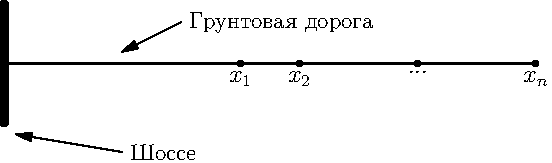
\includegraphics{coop_gadukino.pdf}
\end{figure}

\begin{itemize}
\item Найдите вектор Шепли.
\item Найдите нуклеолус

\item Является ли игра супермодулярной?
\end{itemize}}
\solution{}

\problem{Нефтепровод.

Нефть можно доставить из точки А в точку Б по нефтепроводу. 

\begin{figure}[htbp]
	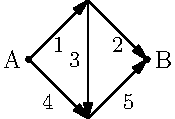
\includegraphics{coop_nefteprovod.pdf}
\end{figure}

Собственники труб и пропускная способность труб в таблице:

\begin{tabular}{|c|c|c|}

\hline 
Номер трубы & Пропускная способность & Владелец \\
\hline
1 & 2 л/час & Андрей \\
2 & 3 л/час & Борис \\
3 & 1 л/час & Володя \\
4 & 2 л/час & Борис \\
5 & 3 л/час & Андрей \\
\hline
\end{tabular}

Потребители нефти готовы платить 1 рубль за скорость передачи 1 литр/час. 
\begin{itemize}
\item Найдите вектор Шепли.
\item Найдите нуклеолус

\item Является ли игра супермодулярной?
\end{itemize}}
\solution{}




\problem{Приведите пример несупераддитивной игры. Желательно не абстрактный, а жизненный. Желательно смешной.}
\solution{Например, Волк, Коза и Капуста. У одного игрока - Волк, у второго - Коза, у третьего- Капуста. Если их владения объединить и не предпринять никаких мер, то стоимость их коалиции ниже суммы их стоимостей.}



\problem{Связь супермодулярности и супераддитивности.

а) Верно ли, что из супермодулярности следует супераддитивность?

б) Приведите пример супераддитивной, но не супермодулярной игры. Желательно не абстрактный, а жизненный. Желательно смешной.}
\solution{a) да}



\problem{ У первого игрока есть $l$ литров левой полуфилософской
жидкости. У второго игрока есть $m>l$ литров правой полуфилософской
жидкости. При смешивании 1 литра левой и одного литра правой полуфилософской
жидкостей получается 1 кг золота. Полуфилосовская жидкость стоит 1
рубль за литр, золото - 3 рубля за килограмм. Полезность от денег
задана функцией $u(m)=\sqrt{m}$. Как поделить полезность между игроками?
(найдите и решение Нэша и решение Калаи-Смородински).}
\solution{}

\problem{
 Рассмотрим коалиционную игру двух игроков в характеристической
форме.

\begin{itemize}
\item Верно ли, что решение Нэша всегда совпадает с вектором Шепли? Докажите
или приведите контр-пример.

\item Верно ли, что решение Калаи-Смородински всегда совпадает с вектором
Шепли? Докажите или приведите контр-пример.

\item Верно ли, что решение Нэша и Калаи-Смородински всегда совпадают? Докажите
или приведите контр-пример.
\end{itemize}}
\solution{}

\problem{ Пусть имеется задача торга $(X,d).$Рассмотрим связанную
с ней некооперативную игру.

Первый игрок предлагает дележ $x^{I}\in X$

Второй игрок предлагает дележ $x^{II}\in X$ и вероятность $p\in[0;1]$.

С вероятностью $p$ игра заканчивается и игроки получают точку несогласия
$d$. С вероятностью $(1-p)$ игра продолжается:

Первый игрок выбирает в качестве финального дележа либо предложенный
им в начале игры дележ $x^{I}$, либо лотерею $px^{II}$. 

Верно ли, что совершенное в подыграх равновесие в этой игре совпадает
с решением Нэша задачи торга? С решением Калаи-Смородински?}
\solution{}

\problem{Докажите, что решение Калаи-Смородинского - единственное
решение, удовлетворяющее условиям эффективности, симметрии, нечувствительности
к смене масштаба, индивидуальной рациональности и индивидуальной монотонности.}
\solution{}

\problem{Какое решение задачи торга получится, если известно, что оно удовлетворяет
условиям индивидуальной рациональности, эффективности, симметрии,
индивидуальной монотонности и независимости от третьих альтернатив?}
\solution{<<По братски>>, т.е. всем поровну.}



\section{Эволюционные игры}
\problem{ Эволюция

Рассмотрим вариант простейшей антагонистической игры <<чет-нечет>>. Два игрока одновременно называют натуральное число. Если сумма чисел четная, то первый игрок выигрывает один рубль, если сумма чисел нечетная, то два рубля выигрывает второй игрок. Для начала найдите равновесие по Нэшу в этой игре. Затем проведите компьютерный эксперимент. Породим на свет 100000 особей, чей генетический код - это играемая особью чистая стратегия. Раунд проходит следующим образом: по очереди каждая особь ... (?)} 
\solution{}





\section{Неразобрано!}








\section{Идеи проектов/курсовых/вопросы с неизвестным (кому?) ответом/конкурсы!}

\problem{ A.Savvateev
Дуополия Бертрана с неодинаковыми издержками,
и/или с ограничением целочисленности цены. Найти
все Нэшевские равновесия. Какие еще могут быть
равновесия?}
\solution{здесь ссылку - где поискать в инете}


\problem{ Приведите пример игры без условия Куна, в которой не существует секвенциального равновесия даже в смешанных стратегиях. (Эта задача довольно зыбкая; ответ мне неизвестен, да и понятие решения там плохо определимо. Однако, если кто продемонстрирует блестящий пример, заработает двойной бонус.) }
\source{НМУ, экзамен 2004, Леша Савватеев}
\solution{мне казалось есть какая-то статья в Journal of gt and ec. beh}





\problem{Конкурс. Лучшая посредственность. Каждому предлагается задумать и подать на
бумаге число от 1 до 100. Тот, чье число ближе всех
к половинке от среднего из названных - победитель.
Призером также является - первым подавший
корректную модель игры.}
\solution{}

 
\problem{ Конкурс. Аукцион <<Лохотрон>>. На столе лежит 100 руб. - дар
экзаменатора. Любой желающий участвовать в
розыгрыше этой купюры вносит на стол 1 рубль
(безвозвратно). Желающие продолжать розыгрыш вносят
еще по 1. И т.д. Победитель забирает все (возместив
экзаменатору 100) и получает "отл.". Призером также
является - первым подавший корректную модель игры.}
\solution{}

\problem{ Конкурс. (<<общее знание>>) Трое или четверо из
занявших лучшие места в другом конкурсе закрывают
глаза и экзаменатор кладет на голову каждому белый
платок. Известно, что платки бывают красные или
белые. Разрешается открыть глаза. Угадать цвет
платка на себе невозможно. Но когда экзаменатор
скажет: "среди вас есть белый платок", угадать
возможно (хотя он ничего нового каждому не
сообщил). Вигрывает угадавший первым и объяснивший.
Призером также является - первым подавший
корректную модель игры.}
\solution{}



\message{ !name(gt_problems_utf8.tex) !offset(-4374) }
